\documentclass[12pt, oneside]{article}   	% use "a msart" instead of "article" for AMSLaTeX format
\usepackage{color}
\usepackage{geometry}                		% See geometry.pdf to learn the layout options. There are lots.
\geometry{letterpaper}                   		% ... or a4paper or a5paper or ... 
%\geometry{landscape}                		% Activate for for rotated page geometry
%\usepackage[parfill]{parskip}    		% Activate to begin paragraphs with an empty line rather than an indent
\usepackage{graphicx}				% Use pdf, png, jpg, or eps§ with pdflatex; use eps in DVI mode
								% TeX will automatically convert eps --> pdf in pdflatex		
\usepackage{amssymb}
\usepackage{amsmath}
\usepackage[compact]{titlesec}
\linespread{1.7}
\usepackage{float}
\usepackage{pdflscape}
%\usepackage{rotating}
\usepackage{soul}
\usepackage{longtable}
\usepackage{caption,setspace}
\captionsetup{font={stretch=1.0}}
%\usepackage{threeparttable}
\usepackage{lineno}
\usepackage[round]{natbib} %round makes parentheses instead of square brackets
\usepackage{url}
%\usepackage{authblk}
\setcounter{secnumdepth}{4}
\titleformat{\paragraph}
{\normalfont\normalsize\bfseries}{\theparagraph}{1em}{}
\titlespacing*{\paragraph}
{0pt}{3.25ex plus 1ex minus .2ex}{1.5ex plus .2ex}
\graphicspath{ {images/} }

\author{}
\author{Allison G.\ Dedrick$^{a, \ast, 1}$ \\
Katrina A.\ Catalano$^a$ \\
Michelle R.\ Stuart$^a$ \\
J.\ Wilson White$^b$ \\
Humberto Montes, Jr.\ $^c$ \\
Malin Pinsky$^a$}

\title{Persistence of a reef fish metapopulation via network connectivity: theory and data}

\date{} 

\begin{document}
\renewcommand{\topfraction}{0.95}
\maketitle{}

\noindent{} a. Department of Ecology Evolution and Natural Resources, Rutgers University, 14 College Farm Road, New Brunswick, NJ 08901 USA;

\noindent{} b. Department of Fisheries and Wildlife, Coastal Oregon Marine Experiment Station, Oregon State University, Newport, OR 97365 USA;

\noindent{} c. Visayas State University, Pangasugan, Baybay City, 6521 Leyte, Philippines

\noindent{} $\ast$ Corresponding author; e-mail: agdedrick@gmail.com

\noindent{} 1. Current address: Stanford Woods Institute for the Environment, Stanford University, Stanford, CA 94305 USA.

% (\textit{Author order not yet determined})

\noindent{\textbf{Running title}}: (45 characters including spaces) Empirical metapopulation persistence

\noindent{\textbf{Keywords}}: metapopulation dynamics, self-persistence, network persistence, \textit{Amphiprion clarkii}, connectivity (5/10)

%\noindent{Current word count}: Introduction - 594, Methods - Results 
\noindent{Statement of authorship}: MLP, JWW, and AGD conceived of and designed the study. MLP, MRS, KAC, and AGD conducted field work and collected data. HRM facilitated field work and provided local ecosystem context and knowledge. AGD analysed the data and wrote the first draft of the manuscript. All authors contributed substantially to revisions. 

\noindent{Data accessibility statement}

\subsection*{Acknowledgements}
We thank Visayas State University for providing logistical support and local ecosystem knowledge during our field sampling in Leyte, Philippines. We particularly thank Geralde Sucano, Jennifer Hoey, Patrick Flanagan, Joyce Ong, Apollo Lizano, Cecil Bantiles, Rodney Silvado, Beverlito Montalban, Teresita Idara, Rogello Nicanor, Liza Espinosa, Shem San Jose, Noel Alquino, Carlos Balasuna, Froilan Beñas, Danilo Marine, Tony Nahacky, and Arturo Bastasa. For financial support, we thank Rutgers School of Environmental and Biological Sciences, NSF \#OCE-1430218, and Alfred P. Sloan Research Fellowship, and an ORAU Ralph E. Powe Junior Faculty Enhancement award. This is publication number \textbf{\#} of PISCO, the Partnership for Interdiscipinary Study of Coastal Oceans, funded primarily by the David and Lucile Packard Foundation.

\bigskip

\section*{Abstract}
Determining whether a metapopulation can persist requires an understanding of both demographic parameters and connectivity among patches. This is well understood in theory but has proved challenging to test empirically. We assessed persistence for a network of patches along a coastline in a metapopulation of yellowtail anemonefish (\textit{Amphiprion clarkii}) using seven years of annual sampling data. We found that this metapopulation produced enough surviving offspring to replace itself but that the spatial pattern of connectivity made it unlikely to persist in isolation despite stable abundances through time. To persist, the metapopulation would need higher fecundity or would need to retain essentially all of the recruits it produced. Increased habitat density alone would not ensure persistence. This first assessment of persistence in a marine metapopulation shows that stable abundance alone is not an indicator of persistence, emphasizing the necessity of untangling demographic and connectivity processes to understand metapopulation dynamics. (138/150 words)

% If submit to Ecology Letters, max 5000 words, 6 figures/tables/text boxes

% \linenumbers{}
% \modulolinenumbers[3]

\section*{Introduction}
The dynamics and persistence of metapopulations depend both on connectivity among patches and on demographic rates within each patch \citep{hastings_persistence_2006, hanski1998metapopulation}. For marine species, connectivity among habitat patches primarily occurs during planktonic larval stages when individuals are hard to track and are able to travel long distances with ocean currents. Because larval connectivity has been perceived to be the greatest uncertainty in these systems, research has centered on quantifying that component \citep[reviewed by][]{white2019connectivity}. More recently, it has become apparent that variation in demographic rates among patches is an equally uncertain aspect of marine metapopulation dynamics \citep{hameed2016inverse, white2011oceanographic}. Given both of those uncertainties, and driven by both fundamental ecological questions and applied needs \citep{botsford_dependence_2001,white_population_2010}, a large body of theory has developed to describe how connectivity and local demography interact to determine whether marine metapopulations persist \citep{burgess2014beyond, botsford2019population}. Testing this theory, however, has proven substantially more difficult.

For any population to persist, individuals must on average replace themselves during their lifetime. Assessing replacement must account for demographic processes across the life cycle, including how likely individuals are to survive to the next age or stage, their expected fecundity at each stage, and the survival to recruitment of any offspring produced. In a spatially structured population, how the offspring are distributed across space is also important \citep{hastings_persistence_2006}. %Marine larvae were once thought to be well-mixed and dispersed far on ocean currents \citep[e.g.][]{roughgarden_recruitment_1988}, suggesting widespread connectivity among patches and largely open populations. Recent advances in estimating connectivity through natural tags and genetics, however, suggest that dispersal may be more limited \citep[e.g.][]{daloia_self-recruitment_2013, hameed2016inverse, almany2017larval}, and local persistence of marine populations on a small spatial scale possible. % Commenting out these sentences right now per Malin's comment that they are similar to the start of the paragraph two down - might revisit and revise

A metapopulation can persist via two mechanisms: 1) at least one patch achieves replacement in isolation, or 2) multiple patches receive enough recruitment to achieve replacement through multi-generational loops of connectivity with other patches in the metapopulation \citep{hastings_persistence_2006, burgess2014beyond}. In the first case (termed self-persistence), enough of the offspring produced at one patch are retained there for it to persist. In the second case (network persistence), closed loops of connectivity among  patches - in which offspring from one patch recruit to another patch but eventually send offspring back to the first in a future generation - provide the patches with enough recruitment to persist within the network. Theory predicts that habitat patches that are large relative to the mean dispersal distance are likely to be self-persistent \citep{white_population_2010}. % Is this sentence relevant here? %If one patch persists, the metapopulation persists.

New ways of identifying individuals and determining their origins now allow better measurements of connectivity in marine populations \citep{almany2017larval, daloia_self-recruitment_2013}. Additionally, a better appreciation of the relevant population dynamic theory has led to measurement of the appropriate demographic factors necessary to assess persistence in field metapopulations \citep{carson2011evaluating, hameed2016inverse, johnson2018integrating, salles_coral_2015}. To date, research has suggested that populations on isolated islands can be self-persistent, which might be expected given that they lack nearby populations from which to receive larvae and would go locally extinct if they did not achieve replacement \cite{salles_coral_2015}. In contrast, small habitat patches spread across a larger reef metapopulation appear to rely on input from surrounding and intervening patches for persistence \citep{johnson2018integrating}. Persistence, however, has yet to be quantified in the field for an entire continuous marine metapopulation, such as all of the patches along a coastline. 

% MOVE TO DISCUSSION PER WILL'S COMMENT ON GOOGLE DOC! % The number of studies estimating demographic rates and connectivity in marine metapopulations is growing \citep{carson2011evaluating, salles_coral_2015, johnson2018integrating, garavelli2018population}, but most use data from one or a few years. Longer data sets enable better estimates of long-term average rates, rather than assuming the demographic and dispersal rates from a particular year or two are representative. Long data sets are also useful for explicitly considering uncertainty, both to assess how well we understand persistence for a population and to assess which parameters contribute most to our uncertainty. Finally, sampling over many years provides abundance trends to compare with persistence metrics.

% Characterizing and understanding variability is important as it can drive dynamics, even allowing persistence when average rates would not (SEBASTIAN CITATIONS), but using data across several years to get a sense of the range of rates and an average is a first step. Having multiple years of data can provide a range of estimates, rather than one point value, and help us understand which parameters contribute most to uncertainty in persistence. 

Here, we further our understanding of metapopulation dynamics in a network of patches along a coastline through a study of yellowtail anemonefish (\textit{Amphiprion clarkii}) in the Philippines. We assessed persistence for all patches of habitat within a metapopulation spread across 30 km of coastline. Based on seven years of data, we found that, despite containing multiple patches with large abundances that were stable over time, the metapopulation was not likely to be persistent and requires immigration from outside patches to persist.% Work on last sentence...

\section*{Methods} 

\subsection*{Persistence theory and metrics}
% For a population to persist, each individual must on average replace itself \citep[e.g.][]{hastings_persistence_2006, botsford2019population}. In non-spatially structured populations, we use criteria such as the average number of recruiting offspring each individual produces during its life (called $R_0$ when the population is age-structured and density-independent) or the growth rate of the population (such as the dominant eigenvalue $\lambda$ of an age-structured Leslie matrix) \citep{caswell_matrix_2001, burgess2014beyond}. For spatially-structured populations, we must also consider the spatial spread of offspring, often represented through a dispersal kernel or connectivity matrix \citep{burgess2014beyond}. %\citep[e.g.][]{cowen_scaling_2006, buston2011probability, hogan_local_2011, daloia2015patterns}). 

%%% RE-ORDER METRICS TO MATCH ORDER OF DETAILED DESCRIPTION BELOW! MOVE LR BACK TO #4!!
We considered four primary metrics to assess whether and how the anemonefish metapopulation was persistent: 1) lifetime recruit production (LRP) to assess whether the metapopulation had enough offspring that survived anywhere to achieve replacement, 3) self-persistence (SP) to assess whether any individual patch could persist in isolation without input from other patches, 3) network persistence ($\lambda_c$) to assess whether the metapopulation was persistent as a connected unit, and 4) local replacement (LR) to assess whether a sufficient number of recruits were retained anywhere within the metapopulation to acheive replacement, without explicitly estimating dispersal. We explain each metric below in detail. To represent the uncertainty in our estimates, we calculated each metric 1000 times, sampling each input parameter from a distribution representing the uncertainty in the empirical estimate (details in \ref{APP_SEC_Uncertainty}). In our results, we show best estimates of each metric with the range of uncertainty values along with uncertainty bounds, defined as the middle 95\% of the distribution of values calculated in this Monte Carlo procedure. % Should this have the \% Reference the section with \ref?

\paragraph*{Lifetime recruit production}
$\text{LRP}_i$ is the expected number of recruits a recruit on patch $i$ will produce in its lifetime,

\begin{equation}
\text{LRP}_i = \text{LEP}_i \times S_e, \label{EQN_LRP}
\end{equation}

where $\text{LEP}_i$ (lifetime egg production) is the patch-specific number of eggs a recruit produces in its lifetime and $S_e$ (egg-recruit survival) is the fraction of eggs that survive to become recruits (Fig.\ \ref{FIG_Schematic}).

If $LRP \geq 1$, individuals produced enough surviving offspring, before considering dispersal, to potentially achieve replacement. If $LRP < 1$, the population could not persist without input from outside patches. We considered all recruits produced by adults in our metapopulation to estimate $\text{LRP}_i$, regardless of where they settled. %This estimates the potential for the entire metapopulation to persist.

\paragraph*{Self-persistence} 

$\text{SP}_i$ is the number of offspring a recruit produces that survive to recruitment and settle in the natal patch,

\begin{equation}
%SP_i &= \text{LEP} \times \text{LR} \\
%SP_i &= \text{LEP} \times S_e \times \frac{p_{i,i} \times \text{\# recruits from patch i}}{S_e \times \text{\# eggs produced by patch i}} \\ 
%SP_i &= \text{LEP} \times S_e \times \frac{p_{i,i} \times \text{\# recruits from site $i$}}{S_e \times \text{\# eggs produced by patch $i$}} \\
%SP_i &= \text{LEP} \times S_e \times p_{i,i}. \label{EQN_SP}
SP_i = \text{LRP}_i \times p_{i,i}, \label{EQN_SP}  % check this...
\end{equation}

where $p_{i,i}$ is the probability of larval retention on patch $i$.

A patch $i$ is self-persistent if $\text{SP}_i \geq 1$. If at least one patch is self-persistent, the metapopulation as a whole persists as well \citep{hastings_persistence_2006, burgess2014beyond}. 

%% MOVE TO SUPPLEMENT!
% Our equation for SP is a modification of that used in \cite{burgess2014beyond}, which uses LEP to represent offspring produced and uses local retention (the number of surviving recruits that disperse back to the natal patch divided by the number of eggs produced by the natal patch) to capture egg-recruit survival and dispersal combined: $\text{LEP} \times \text{local retention} \geq 1$. We modify this to include egg-recruit survival in the offspring term instead, using LRP in place of LEP. %, to assess whether a particular patch $i$ is self-persistent.

\paragraph*{Network persistence}

Network persistence is the largest real eigenvalue $\lambda_C$ of the realized connectivity matrix $C$,

\begin{equation}
C_{i,j} = \text{LRP}_i \times p_{i,j}, \label{EQN_Connectivity_matrix}
\end{equation} 

which we created by multiplying lifetime recruit production ($\text{LRP}_i$) by dispersal probabilities among pairs of patches ($p_{i,j}$) \citep{burgess2014beyond}. The diagonal entries of $C$ are the self-persistence values for each individual patch ($\text{SP}_i$).

Network persistence explicitly considers dispersal of individuals among patches in addition to the reproduction and survival at each patch and requires $\lambda_C \geq 1$ for the network to persist without outside input \citep{hastings_persistence_2006, white_population_2010, burgess2014beyond}.

\paragraph*{Local replacement}

Local replacement (LR) is the number of recruits a recruit produces that return to settle within the focal metapopulation. LR is related to LRP, but LRP, in contrast also includes recruits that settle outside of the focal metapopulation. LR is define as 

\begin{equation}
\text{LR} = \text{LEP}_* \times R_e, \label{EQN_LR}
\end{equation}

where $\text{LEP}_*$ is lifetime egg production averaged across sites and $R_e$ is the proportion of eggs that survived and returned to recruit at the patches in our focal metapopulation (the 30 km section of coastline). $R_e$ is a modification of egg-recruit survival ($S_e$) that implicitly includes dispersal. 
% Like network persistence, local replacement (LR) assesses whether the population is locally self-sustaining. Rather than considering dispersal explicitly as network persistence does, local replacement modifies LRP to estimate the average number of recruits produced per individual that return to settle within our sites. We estimate LR by multiplying LEP by the proportion of eggs produced that survive and return to recruit at our sites ($R_e$), a modification of egg-recruit survival that implicitly includes dispersal. If $LR \geq 1$, individuals produce enough locally-retained offspring to replace themselves and the population can persist in isolation. % One way we assess whether our population is locally self-sustaining is by estimating the number of recruits produced per individual that return to settle within our sites, local replacement (LR).

If $LR \geq 1$, enough offspring were locally retained to achieve replacement if they were evenly spread among patches, but the actual dispersal patterns among the metapopulation patches may still prevent replacement if the pattern of multigenerational replacement does not satisfy the \cite{hastings_persistence_2006} criterion. LR and $\lambda_c$ both assess the ability of our patches to persist as an isolated group but LR treats the network as one large homogenous patch while $\lambda_c$ explicitly accounts for the struture and connectivity among patches.  

\subsection*{Study species}

We focused on a tropical metapopulation of yellowtail anemonefish (\textit{Amphiprion clarkii}, Fig.\ \ref{FIG_Map_and_photo}c). Like many anemonefish species, yellowtail anemonefish have a mutualistic relationship with anemones that house small colonies of fish \citep{buston2003social, fautin1992field}. Yellowtail anemonefish are protandrous hermaphrodites and maintain a size-structured hierarchy; within an anemone, the largest fish is the breeding female, the next largest is the breeding male, and any smaller fish are non-breeding juveniles. The fish move up in rank to become breeders only after the larger fish have died. In the tropical patch reef habitat of the Philippines, yellowtail anemonefish primarily spawn from November to May and lay clutches of benthic eggs that the parents protect and tend \citep{ochi1989mating, holtswarth2017fecundity}. Larvae hatch after about six days and spend 7-10 days in the water column before returning to reef habitat to settle in an anemone \citep{fautin1992field}.

Anemonefish are well-suited to metapopulation studies because dispersal only occurs during the larval phase and adults have limited movement on discete habitat patches (anemones) \citep[e.g.,][]{buston2013marine, salles_coral_2015, almany2017larval}. Yellowtail anemonefish tend to behave more like other reef fishes, with wider-ranging territories and stronger swimming abilities \citep{hattori1991life, ochi1989mating}, than the smaller \textit{A. percula} commonly used in metapopulation studies \citep[e.g.][]{buston2011probability, salles_coral_2015}. %As we show later, survival in yellowtail anemonefish is also lower than \textit{A. percula} and more similar to other damselfishes. 

\paragraph*{Field data collection}

We focused on a set of nineteen reef patches spanning 30 km along the western coast of Leyte island facing the Camotes Sea in the Philippines (Fig.\ \ref{FIG_Map_and_photo}a). The habitat patches covered approximately 20\% of the sampling region and consisted of rocky patches of coral reef separated by sand flats (Fig.\ \ref{FIG_Map_and_photo}a,b). To the north, the patches were isolated from nearby habitat with no substantial reef habitat for at least 20 km, a distance greater than the mean dispersal distance for this species \citep{pinsky2010using}. As such, we considered this to be a relatively isolated metapopulation. Located near a populated coastline, the region experiences anthropogenic effects including fishing, pollution, and runoff from agriculture and a nearby riverbed gravel mine as well as reef-destroying storms like Haiyan and other typhoons in 2013.% Pinsky et al. 2010 paper: (4–27 km with median 11 km)

From 2012-2018, we sampled fish and habitat at most patches each year (Table \ref{APP_TAB_PercHabSampled}). Divers using SCUBA and tethered to GPS readers swam the extent of each patch and visited anemones inhabited by yellowtail anemonefish. At each anemone, the divers caught fish 3.5 cm and larger, took a tissue sample, measured fork length, and noted tail color as an indicator of life stage. Starting in 2015, fish 6.0 cm and larger were also tagged with a passive integrated transponder (PIT) tag unless already tagged. Divers also looked for eggs around each anemone and measured and photographed any clutches found. In total, we took fin clips from and genotyped 2407 fish and PIT-tagged 1930 fish across all years and patches combined, marking 3053 individual fish. % with an average of XX fish clipped and XX fish tagged per year.  % n_offspring_genotyped (785) + n_parents_genotyped (1719) = 2504, not 2772? CHECK!

\subsection*{Estimating demographic and dispersal parameters from empirical data} 

\paragraph*{Parentage analysis and dispersal kernel}  % Check with Katrina/Michelle that this captures the highlights and includes the right references

Over seven years of sampling, we genotyped 1719 potential parents and 785 juveniles at 1340 single nucleotide polymorphisms (SNPs) and found 62 parent-offspring matches \citep{catalanoInPrepconnectivity}. We used a distance-based dispersal kernel fit from the parent-offspring matches \citep{catalanoInPrepconnectivity, bode2018estimating}, where the relative dispersal $p(d)$ is a function of distance $d$ in kilometers and parameters $\theta$ and $z = e^{K_d}$ that control the shape and scale of the kernel (Table \ref{APP_TAB_Params}, uncertainty details in SI \ref{APP_SEC_Uncertainty_Dispersal}). The dispersal kernel estimates the relative dispersal by distance for fish that have survived and recruited so does not separately estimate pre-settlement mortality. To find the probability of fish dispersing among our patches, we numerically integrated the dispersal kernel using the distance from the middle of the origin patch ($i$) to the closest ($d_1$) and farthest ($d_2$) edges of the destination patch ($j$), with distances calculated using the \texttt{geosphere} package in R \citep{geosphere2017R}:

\begin{equation} % might not need this equation...
%p_{A, B}(d) = \int_{d_1}^{d_2} e^k e^{-(e^k d)^\theta}  dd. \label{EQN_integratingDK}
%p_{i, j}(d) = \int_{d_1}^{d_2} z e^{-(zd)^\theta}  dd. \label{EQN_integratingDK}
p_{i,j} = \frac{z\theta}{2\gamma({\frac{1}{\theta})}} \int_{d_1}^{d_2} z e^{-(zd)^\theta}  dd. \label{EQN_integratingDK}
\end{equation}

\paragraph*{Growth and survival: mark-recapture analyses}

Fish marked through geneotyping and PIT tags allowed us to estimate growth and survival through mark-recapture. In total, we had 3053 marked fish with size and stage data for each capture time. 

For growth, we used a von Bertalanffy growth curve
%estimated the parameters of a von Bertalanffy growth curve in the growth increment form relating the length at first capture $L_t$ to the length at a later capture $L_{t+1}$ \citep{hart2009estimating}, where $L_\infty$ is the average asymptotic maximum size across the metapopulation and $K$ is the growth rate: %check that I actually defined those well... % in the growth increment form (according to Hart and Chute) - need to actually get a copy of the Fabens paper, doesn't seem to be available on Google Scholar

\begin{equation} \label{EQN_VBL} 
\begin{split}
L_{t+1} & = L_t + (L_\infty - L_t)[1 - e^{(-k)}] \\
 & = e^{(-k)}L_t + L_\infty[1 - e^{(-k)}],
\end{split}
\end{equation}

where $L_\infty$ is the asymptotic maximum size across the metapopulation and $k$ is the growth rate. We estimated the parameters from the slope $m$ and y-intercept $b$ of the relationship between the length at first capture $L_t$ and the length at a later capture date $L_{t+1}$ for fish recaught after a year (within 345 to 385 days). The von Bertalanffy parameters are $k = -\ln m$ and $L_\infty = b(1-m)$ \citep{hart2009estimating} (Fig.\ \ref{FIG_ParameterInputs}b, Table \ref{APP_TAB_Params}, uncertainty details in SI \ref{APP_SEC_Uncertainty_Growth}).

% From the slope $m = e^{(-K)}$ and y-intercept $b = L_\infty[1 - e^{(-K)}]$, we calculated the von Bertalanffy parameters, such that $K = -\ln m$ and $L_\infty = \frac{b}{(1-m)}$ \citep{hart2009estimating}. We used the first and second capture lengths for fish that were recaught after a year (within 345 to 385 days) to estimate $L_\infty$ and $K$. For fish recaptured more than once, we randomly selected only one recapture period from each to use to estimate the von Bertalanffy parameters and repeated the random selection and estimate 1000 times. We found the mean estimates ($L_\infty$ = 10.70 cm, $K = 0.864$) and mean standard error of those fits, then sampled from within that range to generate a set of von Bertalanffy growth curves to use in our LEP calculations (Fig.\ \ref{FIG_ParameterInputs}b, Table \ref{APP_TAB_Params}, \ref{APP_SEC_METHODS_Growth_and_survival}). 

We used the full set of marked fish to estimate annual survival $\phi$ and probability of recapture $p_r$ using the mark-recapture program MARK implemented in R through the package \texttt{RMark} \citep{RMark_Laake2013}. We fit several models with year, size, and patch effects on the probability of survival on a log-odds scale (see details in SI \ref{APP_SEC_METHODS_Growth_and_survival} and full list of models in Table \ref{APP_TAB_MARKmodels}). The model chosen by $\text{AIC}_c$ indicated that survival differed among patches and increased with fish size (Tables \ref{APP_TAB_Params}, \ref{APP_TAB_SiteSurvivals}, Figs.\ \ref{FIG_ParameterInputs}c, \ref{APP_FIG_SurvBySizeAndSite}, uncertainty details in SI \ref{APP_SEC_Uncertainty_Survival}). 

\paragraph*{Fecundity}

From a regression of eggs per clutch on female size and egg age (determined by the presence of eyed eggs), we determined that fecundity increased with size (eqn.\ \ref{EQN_Fec}, see details in SI \ref{APP_SEC_METHODS_Fecundity}). We only considered reproductive effort once the fish is female and used the average size of first female observation for recaptured fish as the transition size $L_f$ (Fig.\ \ref{FIG_ParameterInputs}d, uncertainty details in SI \ref{APP_SEC_Uncertainty_FemaleSize}).


% %% MOVE THE REST OF THE FECUNDITY SECTION TO SUPPLEMENT!
% We used a size-dependent fecundity relationship determined using photos of egg clutches and females \citep{yawdoszynInPrepfecundity}, where the number of eggs per clutch ($E_c$) is exponentially related to the length in cm of the female ($L$) with size effect $\beta_l = 2.388$, intercept $b = 1.174$, and egg age effect $\beta_e = -0.608$ dependent on if the eggs are old enough to have visible eyes. We multiplied the number of eyed eggs per clutch by the number of clutches per year $c_e = 11.9$ \citep[estimate from][]{holtswarth2017fecundity} to get total annual fecundity $f$ of a female of length $L$:

% \begin{equation}
% f = c_e * e^{\beta_l\ln(L) + \beta_e[\text{eyed}] + b}. \label{EQN_Fec}
% \end{equation}

% \begin{equation} % is this the best way of writing this?
% \ln(E_c) = \beta_l\ln(L) + \beta_e[\text{eyed}] + b. \label{EQN_Fec}
% \end{equation}
% To get total annual fecundity $f$, we multiply the number of eyed eggs per clutch by the number of clutches per year $c_e = 11.9$, using the estimate from \cite{holtswarth2017fecundity}.

% For comparison of numbers (from Clownfish\_SP\_Notes:) Moyer (1986): the individual observed for 11 years and thought to live to at least 13 was ”estimated to have contributed about 160,000 propagules in its lifetime,” spent 3 years as a functional male, then outlived 3 mates as a female; fertilized about 45,000 eggs during 3 years as a male, then spawned about 115,000 eggs as a female; fecundity estimate at this site (Miyake-jima in Japan) is 17,500 eggs/yr/female (from Bell (1976))

\paragraph*{Lifetime egg production (LEP)}

We used an integral projection model (IPM) \citep{ellner2016data} with size as the continuous structuring trait $L$ to estimate lifetime egg production on each patch $i$ ($\text{LEP}_i$). We initialized the IPM with one recruit-sized individual (recruit defined in SI \ref{APP_SEC_METHODS_Recruit_def}) at the initial annual time step ($t=0$), then projected forward for 100 years. We used the size-dependent survival (eqn.\ \ref{APP_EQN_Survival}) and growth (eqn.\ \ref{EQN_VBL}) functions as the probability density functions in the kernel to project the individual into the next time step. The size distribution ($v_z$) at each time step represents the probability that the individual has survived and grown into each of the possible size categories, ranging from a minimum of $L_s=0$ cm to a maximum of $U_s=15$ cm divided into 100 equal size bins. %The probability that the individual is still alive and of any size decreases as the time steps progress; by using a large number of steps, we are able to avoid arbitrarily setting a maximum age and instead let the probabilities become essentially zero. %($\text{size}_\text{recruit}$) 

We then multiplied the size-distribution $v_L$ at each time by the size-dependent fecundity $f$ (eqn.\ \ref{EQN_Fec}) to get the total number of eggs produced at each time step. Integrating across time and size gave the total number of eggs one recruit produced in its lifetime (details in \ref{APP_SEC_METHODS_LEP}, uncertainty details in SI \ref{APP_SEC_Uncertainty_LEP}): % We only considered reproductive effort once the fish was female and used the average size of first female observation for recaptured fish as the transition size ($L_f = 9.32$ cm). Moved this up to fecundity section.

We calculated LEP by site ($\text{LEP}_i$) and averaged across sites ($\text{LEP}_*$) starting for a fish of recruit size. We also calculated LEP averaged across sites for a fish starting a parent size (6.0cm) ($\text{LEP}_p$), used below to estimate egg-recruit survival.


\begin{equation}
\text{LEP} = \int_{t=0}^{100}\int_{L=L_s}^{L=U_s} v_{L,t} f_L dL dt. \label{EQN_LEP}
\end{equation}

\paragraph*{Accounting for density-dependence}  % Should this be its own section or part of the survival from egg to recruit?

We would ideally assess persistence metrics when the population is at low abundance and not limited by density dependence because persistence is defined as having positive population growth at low density; at high density the population growth rate will slow to zero. Density dependence is particularly clear in anemonefish, which have strong social hierarchies. Juveniles on an anemone will prevent others from settling there as well \citep[seen in \textit{A. percula,}][]{buston2003forcible}. Each anemone, therefore, can house only one recently settled anemonefish. This density-dependent mortality artificially reduces the apparent survival of new recruits (recruit defined in SI \ref{APP_SEC_METHODS_Recruit_def}), likely biasing persistence metrics. We accounted for this effect by scaling up our estimate of recruits (the numerator of eqn.\ \ref{EQN_EggRecruitSurv}, described next) by the proportional increase ($\text{DD}$) in unoccupied anemones if all of the anemones occupied by yellowtail anemonefish were unoccupied, where $p_A$ is the proportion of anemones occupied by yellowtail anemonefish and $p_U$ is the proportion of unoccupied anemones: $\text{DD} = \frac{(p_U + p_A)}{p_U} = 1.81$. We present results with this density-dependence modification in the main text and without in the appendix (with subscript DD, Figs.\ \ref{APP_FIG_LRP_LocalReplacement_noDD}, \ref{APP_FIG_SP_NP_realizedCmat_noDD}).

\paragraph*{Survival from egg to recruit ($S_e$)}

We estimated survival from egg to recruit ($S_e$) using parentage matches to find the number of surviving recruits produced by genotyped parents \citep[similar to][]{johnson2018integrating}. However, the number of offspring we assigned back to parents ($R_m = 71$) is a severe underestimate of the offspring produced by genotyped parents because we could not sample exhaustively. To account for offspring missed by our sampling, we divided $R_m$ by four factors (described below and with details in SI \ref{APP_SEC_METHODS_ScalingUpRecruits} and in diagram Fig.\ \ref{APP_FIG_RecruitScalingSchematic}), in addition to multiplying by $\text{DD}$ as described above, then divided by the number of eggs produced by genotyped parents:

\begin{equation}
S_e = \frac{\frac{DD R_m}{P_h P_c P_d P_s}}{N_g \text{LEP}_p}, \label{EQN_EggRecruitSurv}
\end{equation}

where $N_g$ (=1729) was the number of genotyped parents and $\text{LEP}_p$ was the expected lifetime egg production for a fish that has already survived to parent size $p$ (=6.0cm). $\text{LEP}_p$ therefore does not include survival from recruit to parent sizes. $P_h$ (=0.41) was the cumulativeproportion of habitat in our patches that we sampled over time (details in SI \ref{APP_SEC_ProbHabSampled}), $P_c$ (=0.56) was the probability of capturing a fish if we sampled its anemone (details in SI \ref{APP_SEC_ProbR}), $P_d$ (=0.57) was the proportion of the total dispersal kernel area from each of our patches covered by our sampling region (details in SI \ref{APP_SEC_PropDispKernelSampled}), and $P_s$ (=0.20) was the proportion of suitable habitat in our sampling region (details in SI \ref{APP_SEC_PropHabInSampledRegion}).
% We scaled the number of matched recruits by the cumulative proportion of habitat in our sites we sampled over time ($P_h = 0.41$, details in \ref{APP_SEC_ProbHabSampled}), the probability of capturing a fish if we sampled its anemone ($P_c = 0.56$, see \ref{APP_SEC_ProbR} for details), and the proportion of the total dispersal kernel area from each of our sites covered within our sampling region ($P_d =0.57$, calculation in \ref{APP_SEC_PropDispKernelSampled}). Finally, because our dispersal kernel gives the probability of dispersal given that a recruit settled somewhere but our sampling region is not all habitat, we scaled by the proportion habitat in our sampling region ($P_s = 0.20$, details in \ref{APP_SEC_PropHabInSampledRegion}) to avoid counting mortality from settling on non-habitat twice. %P_d was previously 0.57

To estimate the survival and retention of recruits back to our patches (needed for local replacement, LR eqn. \ref{EQN_LR}), we scaled only by $P_h$ and $P_c$: 

\begin{equation}
R_e = \frac{\frac{DD R_m}{P_h P_c}}{N_g \text{LEP}_p}. \label{EQN_Re}
\end{equation}

% We considered uncertainty in the number of offspring assigned to parents during the parentage analysis ($R_m$) and in the probability of capturing a fish ($P_c$). We generated a set of values for the number of assigned offspring using a random binomial, with the number of genotyped offspring (745) as the number of trials and the assignment rate from the parentage analysis (0.079) as the probability of success on each trial \citep{catalanoInPrepconnectivity}. For the probability of capturing a fish, we sampled values from a beta distribution that captures the mean and variance of capture probabilities across recapture dives (details in \ref{APP_EQN_ProbCapBetaDistParams}).

% \paragraph*{Defining recruit and census stage} 

% When assessing persistence, we must consider mortality and reproduction that occurs across the entire life cycle to determine whether an individual is replacing itself with an individual that reaches the same life stage \citep{burgess2014beyond}. We define a recruit to be a juvenile individual that has settled on the reef within the previous year, which also encompasses the size we are first able to sample (3.5-6.0 cm for parentage studies) (Fig.\ \ref{FIG_Schematic}). In theory, it does not matter how we define a recruit as long as we use that definition in our calculations of both egg-recruit survival and LEP. In our system, however, while it is straightforward to calculate LEP from any size, we did not have enough tagged recruits to reliably estimate survival to different recruit sizes. Instead, we choose the mean size of offspring matched in the parentage study as our best estimate of the size of a recruit ($\text{size}_\text{recruit}$) and tested sensitivity to different recruit sizes by sampling from a uniform distribution over the sizes the recruit stage covers (3.5-6 cm, Table \ref{APP_TAB_Params}).

\subsection*{Estimated abundance over time} %%%%% COME BACK AND EDIT/CHECK THIS SECTION!!!%%%%%%%

We examined trends in abundance of breeding females at each patch over time ($F_{i,t}$) to compare to our replacement-based persistence estimates. As with offspring, we scaled up the number of females caught ($F_{c_{i,t}}$) at each patch $i$ in each sampling year $t$ by the proportion of habitat sampled in that patch and year ($P_{h_{i,t}}$) and by the probability of capturing a fish $P_c$:
\begin{equation}
F_{i,t} = \frac{F_{c_{i,t}}}{P_{h_{i,t}}P_c}
%\text{\# females}_{i,t} = \frac{\text{\# females captured}_{i,t}}{P_{h_{i,t}}P_c}. \label{EQN_FemaleAbundance}
\end{equation}

We fit a mixed effects model to estimate the number of fish in each year as a Poisson-distributed variable $\lambda_a$ with effect $m_t$ of year $t$ and with patch as a random effect $m_i$ using the package \texttt{lme4} in R \citep{lme42015package}:

\begin{equation} \label{EQN_Abundance}
\begin{split}
F_{i,0} & \sim Poisson(\lambda_a) \\
F_{i,t} & = (\lambda_a + m_i)m_t t.
\end{split}
\end{equation}

We estimated $\lambda_a$ for an average patch as well as the individual patchs. %The population is increasing over time if $\lambda_a > 1$ and decreasing if $\lambda_a < 1$.
%We fit a mixed effects model to with site as a random effect, estimating the number of fish in each year using the package \texttt{lme4} in R \citep{lme42015package} to assess whether the population trend over time at an average site, as well as the individual sites, is positive or negative. We estimate the number of fish in each year as a Poisson variable with random effects

% \begin{equation}
% %\text{\# females} = m*\text{year} + b. \label{EQN_AbundanceLM}  % There has got to be a better way to write this!
% %\text{\# females}_i \sim \text{year}  % This was what was in the June draft
% \end{equation}

\subsection*{Exploring alternative geographies and larval navigation}

Finally, we tested the sensitivity of metapopulation persistence to patch width and to the proportion of the region that is habitat to understand whether the results would likely be similar in other geographies. We varied the proportion of habitat and the overall width of the region using 19 equally sized and spaced patches with adult survival from the patch with median survival (Elementary School). We created connectivity matrices using the new distances between patches and otherwise used the original parameter values and uncertainty sets. 

We also tested sensitivity to the ability of larvae to navigate to habitat by adding up to a 1km buffer to the edges of the destination patches when integrating the dispersal kernel and adjusting the scaling parameter $P_s$ (eqn.\ \ref{EQN_EggRecruitSurv}) to account for fewer larvae being lost between patches (details in SI \ref{APP_SEC_METHODS_Larval_nav}).

%%%%%%%%% STOPPED EDITING HERE!!
\section*{Results}  
%%%%% MOVE THIS FIRST PARAGRAPH TO SI/ AND/OR INCORPORATE INTO METHODS

% % For our persistence metrics, we present the estimate using the demographic and connectivity input values without uncertainty (the mean of the uncertainty distributions, with the exception of the size range for recruit), as the best estimate and the range with uncertainty shown in brackets. Using our best estimates for growth, survival, and fecundity, w
% We calculated an average value of LEP across sites of 721 eggs [82, 31657] (Fig.\ \ref{FIG_Abun_LEP_LRP_LocalReplacement}b), with values at individual sites that ranged from 0 to 1754 eggs. Uncertainty in adult survival had the largest effect on LEP (Fig.\ \ref{APP_FIG_Uncertainty_LEP}), which corresponds to longer-surviving individuals having more opportunities to reproduce at larger sizes. 

% We estimated egg-recruit survival $S_{e_{DD}}$ to be 0.002 [3.5e-05, 0.014] when we correct for density-dependence in our data. Uncertainty in the size of transition to breeding female $L_f$ had the largest effect on egg-recruit survival (Fig.\ \ref{APP_FIG_Uncertainty_RperE}); the larger the transition size to female, the fewer tagged eggs we estimate were produced by our genotyped parents and the higher our estimate of egg-recruit survival. This differs from our finding above that adult survival had the largest effect on LEP because the starting size of the individual considered is lower when we estimate LEP for a recruit (4.37 cm, 3.5-6.0cm range) than LEP for a parent (6.0cm). Fish considered parents in our parentage analysis have already survived one or more years since recruiting so the transition to breeding female plays a larger role in the number of eggs they are likely to produce than for fish who have just recruited. 

% ADD BRIEF 1-2 SENTENCES REFERENCING MAIN PATTERNS IN FIG 3
\subsection*{Demographic rates}

From field data, mark-recapture, and parentage analyses, we estimated growth, annual survival, and egg-recruit survival. We found an average asymptotic maximum size $L_\infty$ of 10.7 cm, with a growth rate $k = 0.86$ (Fig.\ \ref{FIG_ParameterInputs}b, details in SI \ref{APP_SEC_RESULTS_Growth}). Annual survival varied by site and was higher for larger fish (Figs.\ \ref{FIG_ParameterInputs}c and \ref{APP_FIG_SurvBySizeAndSite}, Table \ref{APP_TAB_SiteSurvivals}, details in SI \ref{APP_SEC_RESULTS_Survival}). Average lifetime egg production across sites ($\text{LEP}_*$) was 827 [227, 2919] (Fig.\ \ref{FIG_Abun_LEP_LRP_LocalReplacement}a, details in SI \ref{APP_SEC_RESULTS_LEP}). Egg-recruit survival was 0.002 [0.0005, 0.01] (details in SI \ref{APP_SEC_RESULTS_Egg-recruit_survival}). \cite{catalanoInPrepconnectivity} estimated the dispersal kernel we used, finding a mean dispersal distance of 8.15 km (Fig.\ \ref{FIG_ParameterInputs}a).

\subsection*{Persistence metrics}

Using our estimates of growth, survival, fecundity, dispersal, and density dependence, we estimated average lifetime recruit production across patches to be 1.74 [0.94, 5.68] (Fig.\ \ref{FIG_Abun_LEP_LRP_LocalReplacement}b). Estimates of $\text{LRP}_i$ at individual patches ranged from 0 to 3.7 (Table \ref{APP_TAB_PatchSpecificLEPandLRP}, Fig.\ \ref{APP_FIG_LRPbySite}). Averaged across patches, 95\% of LRP estimates were $\geq 1$, which means that individuals produced enough offspring to replace themselves. However, LRP does not tell us whether those offspring settled in locations that contributed to persistence.

% For demographic inputs to the persistence metrics, we found that average asymptotic maximum size ($L_\infty$) was 10.70, and annual survival increased with fish size and varied across patches (Figs.\ \ref{FIG_ParameterInputs}c, \ref{APP_FIG_SurvBySizeAndSite}). We estimated average lifetime recruit production (LRP) across patches to be 1.45 with uncertainty bounds of 0.62-7.78 (Fig.\ \ref{FIG_Abun_LEP_LRP_LocalReplacement}c) and best estimates of $\text{LRP}_{i}$ at individual patches ranging from 0 to 3.5. Averaged across patches, 94\% of LRP estimates were $\geq 1$. This means that individuals produced enough surviving offspring to be able to replace themselves. However, LRP does not tell us whether those offspring settled within our sample patches and contributed to persistence. 

%%%%%%%%%% STOPPED EDITING HERE!
Considering retention of larvae at individual patches, we did not find any patches with $\text{SP}_{i} \geq 1$ (Fig.\ \ref{FIG_SP_NP_realizedCmat}a), suggesting that no patch could persist in isolation. The Haina patch came closest to but was still far from self-persistence ($\text{SP}_i = 0.044$ [0.005, 0.23]). % The large uncertainty at Caridad Cemetery stems from the lack of recaptures of marked fish and therefore the high uncertainty in adult survival.

% Text when Haina had an uncertainty range that included >1 (before perc disp kernel sampled was corrected)
% We did not find any sites with a best estimate of $\text{SP}_{DD} \geq 1$ (Fig.\ \ref{FIG_SP_NP_realizedCmat}a), suggesting that none of our sites could persist in isolation. Though the site Haina ($\text{SP}_{DD}$ = 0.055 [2.6e-04, 1.27]) has an SP range that exceeds 1, only 0.1\% of the estimates are $\geq 1$, making self-persistence very unlikely. We also saw estimates $>$ 1 for Caridad Cemetery but those were due to the lack of recaptures at that site and the resulting high uncertainty in adult survival and are unlikely to indicate persistence. I %This suggests that Haina and Wangag could persist on their own at the upper limit of uncertainty in adult survival at the sites, but in general our results do not indicate that any site could perist in isolation. % We see the highest values of self-persistence at our two widest sites Haina (0.13, [XX, XX]) and Wangag (0.082, [XX,XX]), compensating for density-dependence in our data (Fig.\ \ref{FIG_SP_NP_realizedCmat}a). 

% Most of the connectivity in the metapopulation occurred among the patches in the northern and southern areas, from Palanas to Caridad Cemetery and from Tomakin Dako to Sitio Baybayon (Fig.\ \ref{FIG_SP_NP_realizedCmat}b), where the patches tended to be larger, have higher abundances, and have higher survival (Fig.\ \ref{APP_FIG_SurvBySizeAndSite}). The patches with the highest abundances were at the edges of the sampling region and had higher than average LRP so could have exported a substantial fraction of their offspring away the sampling region. % THINK MORE ABOUT WHAT TO SAY HERE!!

For network persistence, our estimate of $\lambda_{c}$ was 0.18 [0.09, 0.63]. None of the uncertainty distribution of $\lambda_c$ was $\geq 1$ (Fig.\ \ref{FIG_SP_NP_realizedCmat}c), suggesting network persistence for this metapopulation was therefore extremely unlikely if not impossible. Our estimate of local replacement (LR) was 0.20 [0.11, 0.65], also suggesting lack of independent persistence of our group of patches and very similar to our $\lambda_{c}$ estimate. While both LR and $\lambda_{c}$ provide information on the ability of our patches to persist as an isolated group, they differ in their assumption of the structure of the population. LR approximates the network of patches as a single well-mixed unit, while $\lambda_{c}$ incorporates the spatial structure of the patches and multi-generation dynamics. 

% , with only a 0.5\% chance $\lambda_{c} \geq 1 = 0.005$ (Fig.\ \ref{FIG_SP_NP_realizedCmat}c). Network persistence for this metapopulation was therefore highly unlikely but not impossible. Our estimate of local replacement LR was 0.16 [0.07, 0.88], also suggesting lack of independent persistence of our group of patchess and very similar to our $\lambda_{c}$ estimate. While both LR and $\lambda_{c}$ provide information on the ability of our patches to persist as an isolated group, they differ in their assumption of the structure of the population. LR estimates the number of recruits individuals at our patches produced that settled within our patches, assuming the network of patches was a single well-mixed unit, while $\lambda_{c}$ incorporates the spatial structure and multi-generation dynamics. % THIS LAST SENTENCE FEELS LIKE IT SHOULD GO IN THE DISCUSSION BUT NOT SURE WHERE...  When we calculated LR using all arriving recruits to our sites, however, rather than just those originating there, our best estimate was $> 1$ (2.08 with 99.8\% estimates $\geq 1$), suggesting that there is recruit-recruit replacement at our sites when we include immigrants. 

\subsection*{Abundance}

Our estimated abundance of females over time had a slight positive trend for the average patch ($m_t = 1.08$, Fig.\ \ref{FIG_Abun_LEP_LRP_LocalReplacement}a), suggesting a slight increase in population size through time. Most individual patches also showed a slight positive trend in female abundance through time, though one large patch (Sitio Baybayon) showed declines (Figs.\ \ref{FIG_Abun_LEP_LRP_LocalReplacement}a, \ref{APP_FIG_AbundanceBySite}s). Therefore, though the metapopulation did not exhibit network persistentence, it also did not show signs of decline over the time scale of our study. 

% This was further confirmed when we calculated LR using all recruits arriving to our patches, rather than just those originating there, assessing whether there was replacement with immigrants included. LR with immigrants gave a best estimate $> 1$ (2.08 with 99.8\% estimates $\geq 1$), also suggesting that there was recruit-recruit replacement for the metapopulation when outside recruits were included.  %% INCLUDE THIS SENTENCE ABOUT LR WITH ALL RECRUITS HERE OR IN THE PARAGRAPH ABOVE?

% Lack of persistence of our sites as a group is also confirmed by our estimate of local replacement ($\text{LR}_{DD}$), which estimates replacement for recruits from our sites returning to our sites, implictly including dispersal, is 0.16 [0.05, 0.76] when we correct for density-dependence in our data. With a value well below one, this suggests individuals at our sites do not replace themselves with recruits that settle in our sites, and that our sites do not persist as an independent network. When we calculated LR using all arriving recruits to our sites, however, rather than just those originating there, our best estimate was $> 1$ (2.06 with XX\% > 1), suggesting that there is recruit-recruit replacement at our sites when we include immigrant recruits.

\subsection*{Alternative geographies}

We then examined what conditions would be needed for this metapopulation to reach persistence. With the existing patch configuration and dispersal kernel, the system would need $\text{LRP} \geq 8.9$ (a five-fold increase) to reach network persistence. In turn, this would require a five-fold increase of egg-recruit survival ($S_e$) or $\text{LEP}_*$ or an equivalent combination of increases across both. Including all arriving recruits as offspring, not just those originating within the metapopulation, LRP would be 11.1, sufficient for persistence. Similarly, our estimate of LR using all recruits arriving to the patches gave an estimate $> 1$ (2.21), also suggesting there was recruit-recruit replacement for the metapopulations when immigrants were included. 

 % NP estimate > 1 when perc_hab = 0.86, 634 runs >= 1 at 0.9 perc hab
Another route to persistence would be with a different dispersal matrix. If dispersal was such that the metapopulation retained all offspring produced, the study region would be persistent because $\text{LRP} > 1$. With the observed dispersal pattern, however, retaining all recruits is difficult to achieve. The coastline had a low fraction of habitat (20\%) and would need to be increased to about 86\% habitat before enough offspring are retained for persistence and the estimate of $\lambda_c > 1$ (with a majority of estimates $\geq 1$, Fig.\ \ref{FIG_WIs}a). However, widening the region while maintaining the same habitat density (20\%) did not achieve persistence (Fig.\ \ref{FIG_WIs}b) unless habitat density was also increased (Fig.\ \ref{FIG_WIs}c). As the region widens, the habitat density necessary for persistence decreases, down to 74\% habitat at a region of 50 km. In contrast, allowing for larval navigation had little impact on persistence estimates (Fig.\ \ref{FIG_WIs}d), as the larger effective area of each patch was essentially offset by removing that area from the scaling that accounted for larval losses to non-habitat ($P_s$ in eqn.\ \ref{EQN_EggRecruitSurv}).

% Another route to persistence would be with a different dispersal matrix. If essentially all recruits produced from our patches landed on one of the outher patches (i.e., none lost to sandy areas between patches or to habitat beyond our study region), the metapopulation would be network persistent because $\text{LRP} \geq 1$. With the observed dispersal pattern, however, retaining all recruits is difficult to achieve. The coastline had a low fraction of habitat (20\%), but increasing this even to 100\% did not achieve network persistence with certainty ($\lambda_c = 0.95$, with only 59\% of the estimates $\geq 1$, Fig.\ \ref{FIG_WIs}a). Essentially all of the offspring produced by the metapopulation need to be retained for a best estimate of persistence, and even with 100\% habitat, many were exported outside of the region. Widening the region at the same habitat density also did not contribute to persistence (Fig.\ \ref{FIG_WIs}b), but persistence became likely for a wider region of 100\% habitat (best estimate $>1$ at about 33 km, Fig.\ \ref{FIG_WIs}c). Allowing for larval navigation hardly changed our persistence estimates (Fig.\ \ref{FIG_WIs}d), as the larger effective area of each patch was essentially offset by removing that area from the scaling that accounted for larval losses to non-habitat ($P_s$ in eqn.\ \ref{EQN_EggRecruitSurv}).

% Old text from when
%Alternately, increasing the amount of habitat in our region (currently about 20\%) to 55\%, with equally sized and spaced sites with adult survival of an average site, gives a best estimate of $\lambda_{c_{DD}} = 1$ and suggests network persistence (Fig.\ \ref{FIG_WI_PERC_HAB}a). Considering uncertainty, 95\% of the estimates of $\lambda_{c_{DD}}$ are $> 1$ at about 85\% habitat (Fig.\ \ref{FIG_WI_PERC_HAB}b).

% Our estimated abundance of females over time has a slight positive trend for the average site ($m_t = 1.08$, Fig.\ \ref{FIG_Abun_LEP_LRP_LocalReplacement}a), suggesting a slight increase in population size for the population overall through time. Most individual sites also show a slight positive trend in female abundance through time, though one large site shows declines (Fig.\ \ref{FIG_Abun_LEP_LRP_LocalReplacement}a, Fig.\ \ref{APP_FIG_AbundanceBySite}s). %COME BACK AND CHECK AND DEAL WITH THIS!

\section*{Discussion}

In this first assessment of demographic persistence of a coastal marine metapopulation, we did not find strong evidence for either self-persistence of an individual patch or network persistence of the entire 30 km area as an isolated region. This inability to persist as an isolated region does not mean that the metapopulation was declining, however. Both population trends and replacement of recruits with immigrants showed that population levels were stable or increasing slightly. Taken together, these metrics suggest that the region required input of immigrants to persist. Despite encompassing a distance substantially larger than mean dispersal, the coastline only persisted as part of a larger metapopulation.

Theory for predicting persistence within patchy habitats has suggested that we expect self persistence for patches with a length at least twice the mean dispersal distance \citep{lockwood2002effects} and network persistence from groups of patches where the proportion of habitat is about 10-40\% \citep[depending on the particular species, population, and the steepness of the stock-recruit curve, ][]{botsford2019population}. Individual patches in the focal metapopulation where too small for self-persistence, but the 30 km region we sampled was about triple the mean dispersal distance of yellowtail anemonefish estimated from previous genetic work \citep[around 9 km,][]{pinsky2010using} and from our parentage analyses \citep[8.2 km,][]{catalanoInPrepconnectivity}. Rather than a continuous patch, however, the region was only about 20\% habitat. This low value may result at least in part from habitat declines over recent decades, based on interviews with fishers in the early 2000s (Jennifer Selgraeth, pers.\ comm.\ ). Increasing the proportion of coastline with habitat in sensitivity tests, however, suggested that 40\% habitat coverage would not be sufficient to achieve persistence and this metapopulation would require at least 86\% habitat to persist. Similar to fish on small patches in the Caribbean \citep{johnson2018integrating}, this anemonefish metapopulation depends on the production and connectivity of outside patches. One possible path to persistence would be through nearby patches that had higher egg production or survival. In such a case, even a small increase in area could create a persistent network. Deeper reefs, for exampe, often have better reef health than shallower reefs \citep{cinner2016bright} - $\text{LRP}_i$ is highest at our deepest patch, Tomakin Dako. In our system, offshore reefs at Cuatro Islas or the Camotes Islands, for example, with higher coral cover and less silt, could have higher anemonefish survival and contribute disproportionately to regional metapopulation persistence.

% or Botsford ref in discussion: make it vaguer - something like “expect self persistence as the patch size increases, expect network persistence if the proportion habitat is about 0.1-0.4”, cite Loo, Will, Alan 2019 book. Can put a parenthetical saying it depends on the particular species, population and the steepness of the stock-recruit curve (also see Will email for details)

% From theory for predicting persistence within marine protected areas, we expect persistence in patches with a length at least twice the mean dispersal distance \citep[e.g.][]{lockwood2002effects} or from a network of patches when at least 35\% of the coastline is habitat \citep{botsford2001dependence}. Our individual patches were likely too small for self-persistence but the 30 km region we sampled was more than twice the mean dispersal distance of yellowtail anemonefish estimated from previous genetic work \citep[9 km,][]{pinsky2010using} and our samples \citep[8.2 km,][]{catalanoInPrepconnectivity}. Rather than a continuous patch, however, the region was only about 20\% habitat and experienced declines in habitat extent and quality in recent decades (fishers noticed habitat changes when asked in the early 2000s, Jennifer Selgreth, pers.\ comm.). Poor habitat quality limited persistence; even 100\% habitat did not guarantee network persistence in our sensitivity test, unless the region was also larger. Low production means that the area required for the larger persistent metapopulation \cite[like][estimated in their system]{johnson2018integrating} depends on the production and connectivity of outside patches. If surrounding patch populations had a similar LRP and level of connectivity as our patches, increasing the area of the network to include them would not achieve network persistence, as seen in our simulation of a wider region with the sampling region habitat density and quality. If nearby patches had higher egg production or survival, however, a small increase in area could create a persistent network. Nearby reef patches such as Cuatro Islas, for example, with higher coral cover and less silt, could have had higher survival and contributed recruits to our patches. 

% From theory for predicting persistence within marine protected areas, we expect persistence in patches with a length at least twice the mean dispersal distance \citep[e.g.][]{lockwood2002effects} or from a network of patches when at least 35\% of the coastline is habitat \citep{botsford2001dependence}. Our individual patches were likely too small for self-persistence but the 30 km region we sampled was more than twice the mean dispersal distance of yellowtail anemonefish estimated from previous genetic work \citep[9 km,][]{pinsky2010using} and our samples \citep[8.2 km,][]{catalanoInPrepconnectivity}. Rather than a continuous patch, however, the region was only about 20\% habitat and experienced declines in habitat extent and quality in recent decades (fishers noticed habitat changes when asked in the early 2000s, Jennifer Selgreth, pers.\ comm.). Poor habitat quality limited persistence; even 100\% habitat did not guarantee network persistence in our sensitivity test, unless the region was also larger. Low production means that the area required for the larger persistent metapopulation \cite[like][estimated in their system]{johnson2018integrating} depends on the production and connectivity of outside patches. If surrounding patch populations had a similar LRP and level of connectivity as our patches, increasing the area of the network to include them would not achieve network persistence, as seen in our simulation of a wider region with the sampling region habitat density and quality. If nearby patches had higher egg production or survival, however, a small increase in area could create a persistent network. Nearby reef patches such as Cuatro Islas, for example, with higher coral cover and less silt, could have had higher survival and contributed recruits to our patches. 

Our finding of a lack of isolated persistence of differs markedly from persistence findings of other reef fish metapopulations. On reefs surrounding Kimbe Island, \cite{salles_coral_2015} report self-persistence of individual anemonefish subpopulations in lagoons that were of similarly size (approximately 100-500 m long) to our individual patches, as well as network persistence of the only 800 m wide metapopulation around the island. This persistence finding is at a dramatically smaller scale than for our focal population in the Philippines. Additionally, \cite{johnson2018integrating} estimated that four reefs of a combined area of only 2.6 $\text{km}^2$ (4 65 ha patches) would be sufficient for network persistence of a damselfish metapopulation across multiple islands in the Bahamas. This area is equivalent to a coastline section shorter than our sampling region (approximately 30 km long and 0.1 km wide). To persist, these two offshore metapopulations either had much higher retention of recruits or higher LRP than did our coastline patches. Though lack of sufficient connectivity and retention is thought to inhibit network persistence in some systems \citep[e.g., insufficient retention of offspring within reserves for eastern oysters (\textit{Crassostrea virginica}) in North Carolina;][]{puckett2016metapopulation}, production of surviving recruits seems the likelier explanation in this case. Recruit production was lower in the Philippines than in the Kimbe Island populations, where estimates of lifetime reproductive succes that included dispersal to the natal reef \citep{salles2020strong} were higher than our estimates of LRP without dispersal losses (LRP of 1.74). Lower LRP at our sites could be due to lower egg production, slower growth, or lower adult survival, all likely affected by habitat quality \citep[e.g.][]{salles2020strong, hayashi2019low}. Our study system was near a populated coastline and experienced anthropogenic effects, including pollution and silt, that can reduce demographic rates. Adult survival, for example, was lower at the two patches just downstream of the gravel mine (N. and S. Magbangon in Fig. B.3). Even at our higher-survival sites, survival was lower than estimates from the populations at Kimbe Island \citep[85\% annual survival,][]{salles_coral_2015}. Metapopulation studies in other reef fish \citep[e.g.][]{figueira2009connectivity} and marine species more broadly \citep{carson2011evaluating} are highly sensitive to adult survival and other demographic parameters.
%%%%%%%% NEED TO ADD IN SURVIVALS AND KIMBE BAY LRP equivalent! survival for a 6.0cm fish at Tomakin Dako is 38%, 27% at Elementary School, 10% at N. Magbangon (lowest); for 9 cm fish 15% at N. Magbangon, 37% at Elementary School, 53% at Tomakin Dako
%%%%% STOPPED EDITING HERE!!
Temporal variability in demographic or dispersal parameters on a time scale longer than our sampling alternatively could have enabled persistence of our patches in isolation \citep[similar to the storage effect,][]{warner1985coexistence} rather than as part of a larger metapopulation. Successful recruitment events on the decadal scale, for example, sustain rockfish populations on the west coast of the United States through the intervening weak recruitment years \citep[e.g.][]{tolimieri2005roles}. Our study could have missed a particularly strong recruitment event driven by variable ocean connectivity \citep[simulations suggest that 20 years are necessary to capture the full extent of ocean variability in the Coral Triangle region surrounding our patches;][]{thompson2018variability}. Strong recruitment would need to occur at least once a generation to maintain patch populations without switching to colonization and extinction dynamics, however, which we do not see. Our study likely spans the generation time of a yellowtail anemonefish (roughly 5 years) so variable strong recruitment, while possible, is unlikely to sustain our populations.

Understanding our region in the context of broader metapopulation theory requires reconciling replacement-based persistence analysis with classic colonization-extinction and source-sink dynamics. At the patch level, many marine metapopulations do not exhibit the colonization-extinction dynamics \citep[or do only on a decades to centuries timescale,][]{smedbol2002myths} more common in terrestrial metapopulations \citep[e.g. in butterflies and pikas;][]{hanski1998metapopulation, moilanen1998long} and instead consist of continuously occupied patches connected by dispersal \citep{kritzer2006marine} that are not necessarily easily classified as sources or sinks. Despite being unable to persist in isolation, our region is not technically a sink \citep{pulliam1988sources} because LRP $> 1$. For these metapopulations, lack of self-persistence can have two causes: reproduction does not balance mortality losses within a patch (as in a sink) or sufficient recruits are produced but not retained (as we see in our region). Dispersal that leads to demographic exchange rather than colonization is not commonly considered in classic metapopulation dynamics, though there have been some attempts to include all successful offspring from a patch and not just those retained locally when classifying sources and sinks \citep{figueira2006defining}. Many metapopulations likely lie on a continuum between extinction-colonization dynamics and exchange among populated patches \citep{kritzer2006marine}, and bridging these metapopulation views could lead to a more complete understanding of persistence in patchy and variable environments.

Our sampling on patchy coral reefs was designed for mark-recapture analysis rather than a comprehensive habitat or abundance census, so though we accounted for uneven sampling, we could have missed population declines if the underlying habitat was shifting. We used tagged anemones to account for unvisited patch habitat, but tags with missing anemones are harder to find. If anemones disappeared over time at our patches, we could have overestimated the number of fish and missed population declines indicating lack of persistence even with outside input. These scaling challenges are not unique to our study: few ecological studies are full censuses through time, and marine metapopulations tend to be patchy and heterogeneous \citep[e.g. coral reefs, the intertidal zone, and kelp forests;][]{saenz2011connectivity, johnson2001metapopulation, castorani_connectivity_2015}, where individuals are not well-mixed across space or time. In these cases, carefully considering how sampling interacts with distribution, properly accounting for such uncertainties, and characterizing uncertainty in parameter estimates, is an important part of persistence estimation.

Density-dependence also presents a sampling challenge. Persistence criteria \citep{hastings_persistence_2006, burgess2014beyond} ask whether a population at low abundance can grow and recover rather than going extinct. Density-dependence is often ignored at low abundances \citep{botsford2019population} so is not explicitly considered in persistence metrics. In real populations, however, it can be challenging to estimate density-independent demographic rates, as density-dependence is occurring in the population as it is sampled in processes such as dispersal \citep[e.g. in butterflies,][]{nowicki2011evidence} and fecundity \citep[e.g. in warblers,][]{rodenhouse2003multiple}. In yellowtail anemonefish, density-dependence is likely most important immediately post-settlement, as it is for many species \citep[e.g. corals, trees, and butterflies;][]{vermeij2008density, harms2000pervasive, nowicki2009relative}, but could continue to be important throughout the life history due to social hierarchies in anemonefish colonies \citep[e.g.][]{buston2011determinants}. To avoid competition within the colony, fish in the pre-reproductive queue may have lower growth and survival than fish alone on an anemone \citep[seen in \textit{A. percula},][]{buston2003social, buston2003forcible}, suggesting higher growth and survival, and therefore LRP, in the absence of density-dependence.

Understanding persistence is critical for the management of spatial populations, such as siting marine protected areas \citep[e.g.][]{kaplan_model-based_2009}, assessing habitat fragmentation risks \citep[e.g.][]{smith2002population, fahrig2001much} and conserving species in the face of climate change \citep[e.g.][]{coleman2017anticipating, fuller2015persistence}. Though models and theory provide us with expectations, we are only recently beginning to be able to tackle these questions of persistence empirically in model systems such as anemonefish and other sedentary tropical reef fish \citep[e.g.][]{salles_coral_2015,johnson2018integrating}. With parentage analyses now being extended to temperate marine species \citep[e.g.][]{baetscher2019dispersal} and a better understanding of how biophysical models compare to larval dispersal patterns \citep{bode2019validation}, we are beginning to move beyond model species and investigate persistence in harvested and spatially-managed systems \citep[e.g.][]{garavelli2018population}. Our study shows the importance of long term sampling and careful consideration of the different demographic processes that affect our metric calculations, such as density-dependence and sampling biases, to distinguish persistence ability from population trajectories and understand marine population dynamics in empirical systems.

% \section*{Discussion}
% % FIT THIS INTO DISCUSSION? 
% % MOVE TO DISCUSSION PER WILL'S COMMENT ON GOOGLE DOC! % The number of studies estimating demographic rates and connectivity in marine metapopulations is growing \citep[e.g.][]{carson2011evaluating, salles_coral_2015, johnson2018integrating, garavelli2018population}, but most use data from one or a few years. Longer data sets enable better estimates of long-term average rates, rather than assuming the demographic and dispersal rates from a particular year or two are representative. Long data sets are also useful for explicitly considering uncertainty, both to assess how well we understand persistence for a population and to assess which parameters contribute most to our uncertainty. Finally, sampling over many years provides abundance trends to compare with persistence metrics.

% In this first assessment of demographic persistence of a coastal marine metapopulation, we did not find strong evidence for either self-persistence of an individual patch or network persistence of the entire 30 km system as an isolated region. This inability to persist as an isolated region does not mean that the metapopulation is declining, however. Population trends - both abundance over time and replacement of recruits with immigrants included - find that population levels are stable or increasing slightly. Taken together, these metrics suggest that the region has a stable population on average but requires input of immigrants to persist. Despite encompassing a distance larger than mean dispersal, the coastline only persists as part of a larger metapopulation.

% For the anemonefish metapopulation to persist as an isolated network, either the number of surviving recruits produced by an average recruit (LRP) would need to be about six times higher (about XX) or more recruits would need to be retained within the region. This higher LRP value is similar to estimates of lifetime reproductive success that include dispersal to the natal reef in a clownfish on an isolated island \citep{salles2020strong}, suggesting it is not an unreasonable level of production. Habitat quality affects production in reef fishes \citep[e.g.,][]{salles2020strong, hayashi2019low}, and our study system is near a populated coastline and experiences anthropogenic effects, including pollution and silt from a riverbed gravel mine. Adult survival, for example, was lower at the two patches just downstream of the gravel mine (N.\ and S.\ Magbangon in Fig.\ \ref{APP_FIG_SurvBySizeAndSite}), with impacts on $\text{LEP}i$ and therefore $\text{LRP}_i$. 

% Alternately, higher connectivity and retention of offspring among patches could lead to network persistence. Though lack of sufficient connectivity and retention is thought to inhibit network persistence in other systems \citep[e.g., a collection of reserves for eastern oysters (\textit{Crassostrea virginica}) in the Pamlico Sound in North Carolina;][]{puckett2016metapopulation}, low production of surviving recruits due to poor habitat quality seems the more likely explanation in our system. Our dispersal kernel is comparable to those estimated for other species of reef fish, both similar in shape \citep[e.g.,][]{harrison2012larval, daloia2015patterns} and with a mean dispersal distance of a similar range to that estimated for \textit{A. percula} in Kimbe Bay \citep[13.3 and 18.9 km compared to our estimate of 8.2 km;][]{almany2017larval}, which has been found to be persistent without input from outside reefs \citep{salles_coral_2015}. 

% % What-ifs, habitat amount
% We do not find clear evidence for network persistence despite estimates of the mean dispersal distance of \textit{A. clarkii} from previous genetic work \citep[9 km,][]{pinsky2010using} and from our samples \citep[8.2 km,][]{catalanoInPrepconnectivity} that are well within the 30 km span of our patches. The length of the metapopulation is more than twice the mean dispersal distance, usually sufficient for persistence of a population in an isolated habitat patch \citep[e.g.,][]{lockwood2002effects}. However, the metapopulation contains only about 20\% habitat, rather than a continuous stretch, which may be too low to support network persistence. Habitat quality and extent in our region has likely been declining in recent decades. The region was hit in 2013 by Typhoon Haiyan, one of the strongest typhoons ever to make landfall, which destroyed reef habitat, including one of our northern sampling patchess. Fishers also noticed prior habitat changes when asked in the early 2000s (Jennifer Selgreth, pers. comm.). Finally, agriculture has spread over much of the steep mountain slopes immediately east of the metapopulation, possibly leading to extensive runoff over historical time and loss of reef habitat along this coastline. Our simulations suggests that even 100\% habitat in our sampling region does not guarantee network persistence.

% In addition, individual patches are too small to reach self-persistence. The largest patch, Haina, is only 0.8km wide, about 10 times smaller than the mean dispersal distance. This is in contrast to findings on isolated reefs surrounding Kimbe Island, however, where several anemonefish subpopulations in lagoons of similar size as our patches were found self-persistent \citep{salles_coral_2015}. The suggestion of a habitat shortage in our sampling region is partially dependent on our assumption that larvae land in non-habitat between patches and die. Larvae have some navigational and habitat-finding capabilities \citep[e.g.][]{elliott1995host, fisher2005swimming}, so we could be underestimating their ability to find habitat in our calculations, which would decrease the amount of habitat required for network persistence. % In our site with the highest LEP, a width of XX would be required for self-persistence.  COME BACK AND DEAL WITH LARVAL NAVIGATION AND THIS PARAGRAPH!!

% We suggest that this metapopulation is a sink area of a larger metapopulation but the area required for the larger persistent metapopulation depends on the production and connectivity of outside patches. If surrounding patch populations have a similar LRP and level of connectivity as our patches, increasing the area of the network to include them also would not achieve network persistence. If nearby patches have higher egg production or egg-recruit survival, however, it might not take much of an increase in area considered to create a persistent network. Nearby reef patches such as Cuatro Islas, for example, with higher coral cover and less silt, could have higher survival of fish and be contributing recruits to our patches. % COULD CONSIDER ADDING BIT ABOUT POLLUTION HERE INSTEAD OF IN LRP PARAGRAPH ABOVE. ANYTHING WE CAN SAY ABOUT THE SCALE OF OTHER METAPOPS AS A COMPARISON?

% An alternative to our sampled patches existing as a sink portion of a larger metapopulation is that variability in demography or dispersal on a longer scale than our sampling time could lead to persistence \citep[similar to the storage effect,][]{warner1985coexistence} For example, rockfish on the west coast of the United States have highly variable and episodic recruitment, where successful recruitment events occur on the decadal scale and sustain the population until the next strong recruitment event \citep[e.g.,][]{tolimieri2005roles}. Though perhaps not as extreme as in the California Current system, ocean connectivity is still variable in the Coral Triangle region surrounding our study patches, with estimates suggesting that 20 year simulations are necessary to capture the full extent \citep{thompson2018variability}. Our study, though relatively long term, could have missed a particularly strong recruitment event that would enable local persistence of the set of populations we sampled. 

% Though we estimate abundance trends and do not find overall declines, it is possible we could have missed declines due to our sampling design. Our sampling study was designed for mark-recapture analyses rather than a comprehensive habitat or abundance estimate so we did not sample all areas of all patches each year. We scaled up the number of fish we caught to account for those we missed using the proportion of tagged anemones we visited, which assumes that all tagged anemones are equally likely to be sampled. In reality, tags that no longer have anemones next to them are likely harder to find and sample. If anemones are disappearing over time at our patches, we might be overestimating the number of fish present and missing population declines at our patches that would mean lack of persistence even with outside input. Properly accounting for such uncertainties, and characterizing uncertainty in our parameter estimates, is an important part of persistence estimation.

% % Including uncertainty in our empirical estimates of demographic and dispersal parameters allows us to better understand how likely it is that the population is persistent and which processes contribute the most uncertainty. We see a wide range of estimated metric values, spanning of network persistence for our set of sites to far from it. In our study, demographic parameters, particularly adult survival, have a large effect on whether or not we think the population is persistent. Other metapopulation studies also find higher sensitivity to demographic rather than connectivity parameters \citep[e.g., on source or sink status in bicolor damselfish;][]{figueira2009connectivity}, including particular sensitivity to adult survival \citep[on metapopulation growth rate in mussels;][]{carson2011evaluating}. Our estimates of connectivity are simpler than our estimates of demography, with no spatial variability \citep[which can be important in understanding demographic connectivity;][]{johnson2018integrating}, and a more thorough assessment could alter their relative effect on persistence, but this suggests that sufficient offspring production and survival has a larger effect on persistence at these relatively small scales of connectivity. Uncertainty in our sampling, particularly how likely we are to capture a fish, however, contributes the most uncertainty to whether we determine the population to be persistent, highlighting the challenge of estimating these metrics empirically. For a marine metapopulation, our system is relatively uncomplicated; as we accumulate more empirical assessments of metapopulations to compare to our expectations from theory and models, we will have to think carefully about how to handle uncertainty as we move to tackling larger and more complicated systems.

% % Caveats - density-dependence
% Persistence criteria \citep{hastings_persistence_2006, burgess2014beyond} ask whether a population at low abundance can grow and recover rather than going extinct. Density-dependence is often ignored at low abundances \citep{botsford2019population} so is not explicitly considered in persistence metrics. In real populations, however, it can be challenging to estimate density-independent demographic rates, as density-dependence is occurring in the population as it is sampled in processes such as dispersal \citep[e.g. in butterflies,][]{nowicki2011evidence} and fecundity \citep[e.g. in warblers,][]{rodenhouse2003multiple}. In yellowtail anemonefish, density dependence is likely most important immediately post-settlement, as it is for many species \citep[e.g. corals, trees, and butterflies:][]{vermeij2008density, harms2000pervasive, nowicki2009relative}, but could continue to be important throughout the life history due to social hierarchies in anemonefish colonies \citep[e.g.][]{buston2011determinants}. To avoid competition within the colony, fish in the pre-reproductive queue may have lower growth and survival than fish alone on an anemone \citep[seen in \textit{A. percula},][]{buston2003forcible, buston2003social}, suggesting higher growth and survival, and therefore LRP, in the absence of density-dependence.
% % %% CONDENSE INTO 1-2 SENTENCES, INCLUDE MORE DISCUSSION OF DD IN OTHER SYSTEMS AND WHAT IT MEANS FOR PERSISTENCE MEASUREMENT (RIGHT NOW TOO FOCUSED ON RESULTS, NOT ENOUGH ON IMPLICATIONS)
% % Density-dependence could continue to be important throughout the life history, however, due to the social hierarchies in colonies of clownfish \citep[e.g.][]{buston2011determinants}. In other species of clownfish, individuals on the same anemone maintain strict size spacing, restricting their food intake and growth to avoid encroaching on the position of another fish and being attacked or evicted \citep[seen in \textit{A. percula},][]{buston2003forcible, buston2003social}. This suggests that while fish are in the pre-reproductive queue, density-dependence may lower growth rates compared to the growth of fish alone on an anemone, as would be the case in a population at low abundance. We include the primary effect of density-dependence on our estimate of egg-recruit survival but other estimates, particularly growth and survival, would also likely be higher in the absence of density-dependence and increase LRP.

% Understanding persistence is critical for the management of spatial populations, such as siting marine protected areas \citep[e.g.,][]{kaplan_model-based_2009}, assessing habitat fragmentation risks \citep[e.g.,][]{smith2002population, fahrig2001much} and conserving species in the face of climate change \citep[e.g.,][]{coleman2017anticipating, fuller2015persistence}. Though models and theory provide us with expectations, we are only recently beginning to be able to tackle these questions of persistence empirically in model systems such as clownfish and other sedentary tropical reef fish \citep[e.g.,][]{salles_coral_2015, johnson2018integrating}. With parentage analyses now being extended to temperate marine species \citep[e.g.,][]{baetscher2019dispersal} and a better understanding of how biophysical models compare to larval dispersal patterns \citep{bode2019validation} we are beginning to move beyond model species and investigate persistence in harvested and spatially-managed systems \citep[e.g.,][]{garavelli2018population}. Our study shows the importance of long term sampling and careful consideration of the different demographic processes that affect our metric calculations, such as density-dependence and sampling biases, to distinguish persistence ability from population trajectories and understand marine population dynamics in empirical systems.

\newpage{}

\section*{Figures}

% Figure 1 - metrics and life cycle schematics
\begin{figure}[H] % metric schematic and life cycle schematics
	\centering
	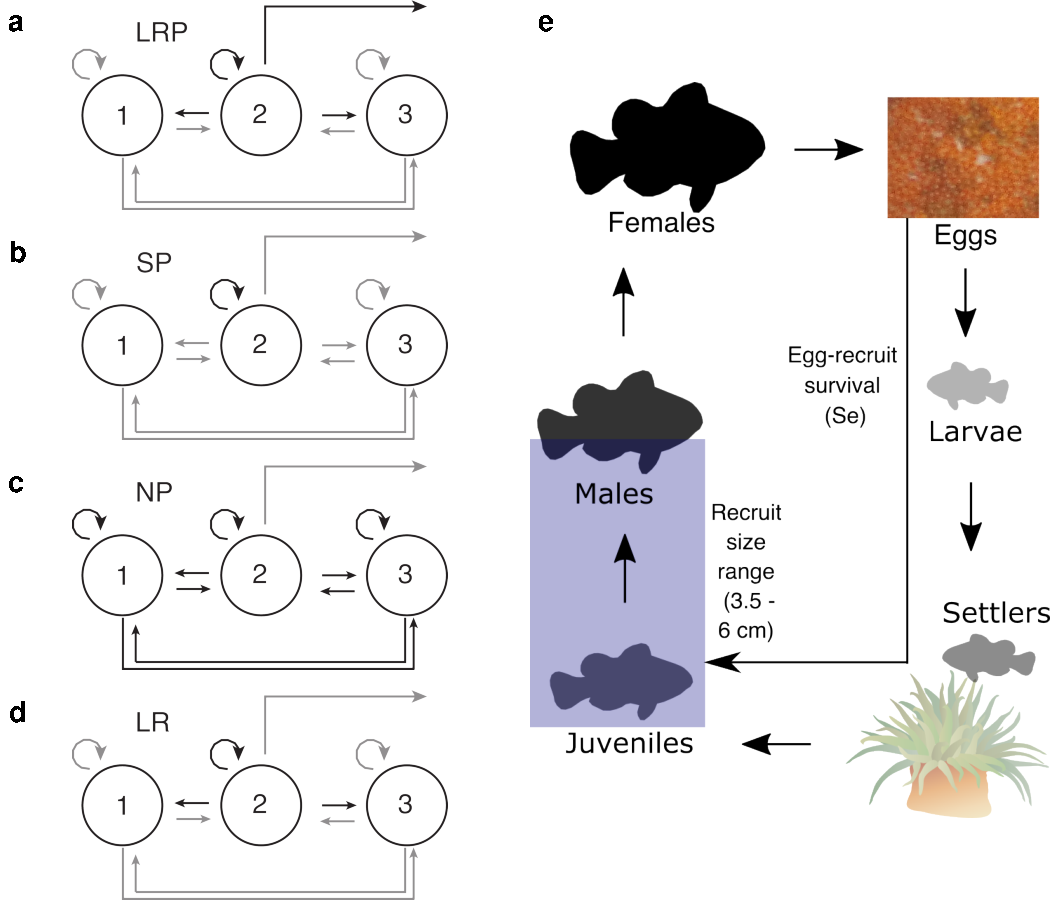
\includegraphics[width = 1.0\textwidth]{\detokenize{../Plots/LifeCycleSchematic/metrics_life_cycle_schematics.pdf}}
	\caption{Schematics of the persistence metrics (a-d): a) lifetime recruit production (LRP, eqn.\ \ref{EQN_LRP}), b) self-persistence (SP, eqn.\ \ref{EQN_SP}), c) network persistence (NP, first eigenvalue of eqn.\ \ref{EQN_Connectivity_matrix}), and d) local replacement (LR, eqn.\ \ref{EQN_LR}). e) The life cycle of yellowtail clownfish, including the range of sizes considered recruits (recruit definition in SI \ref{APP_SEC_METHODS_Recruit_def}). \label{FIG_Metric_life_cycle_schematics}} 
\end{figure}

% Figure 2 - map + photo
\begin{figure}[H] % Map + clownfish photo
	\centering
	\includegraphics[width = 1.0\textwidth]{\detokenize{../Plots/FigureDrafts/Map_and_photo_2.pdf}}
	\caption{a) Map of the patches along the coast of Leyte in the Philippines. From north to south, the patches are: 1) Palanas, 2) Wangag, 3), North Magbangon, 4) South Magbangon, 5) Cabatoan, 6) Caridad Cemetery, 7) Caridad Proper, 8) Hicgop South, 9) Sitio Tugas, 10) Elementary School, 11) Sitio Lonas, 12) San Agustin, 13) Poroc San Flower, 14) Poroc Rose, 15) Visca, 16) Gabas, 17) Tomakin Dako, 18) Haina, and 19) Sitio Baybayon. b) Zoomed-in map of the northern-most patch, Palanas, to show anemone arrangement with anemones colored as occupied by \textit{A.\ clarkii} (green) or unoccupied by anemonefish (orange). c) An example anemone occupied by \textit{A.\ clarkii} in a typical habitat at the patches. The metal anemone tag is visible just above the anemone on the rock.  \label{FIG_Map_and_photo}} 
\end{figure}

% Figure 3 - demographic and dispersal inputs
\begin{figure}[H] % demographic parameters: survival curve, growth curve, dispersal kernel, transition size to female 
	\centering
	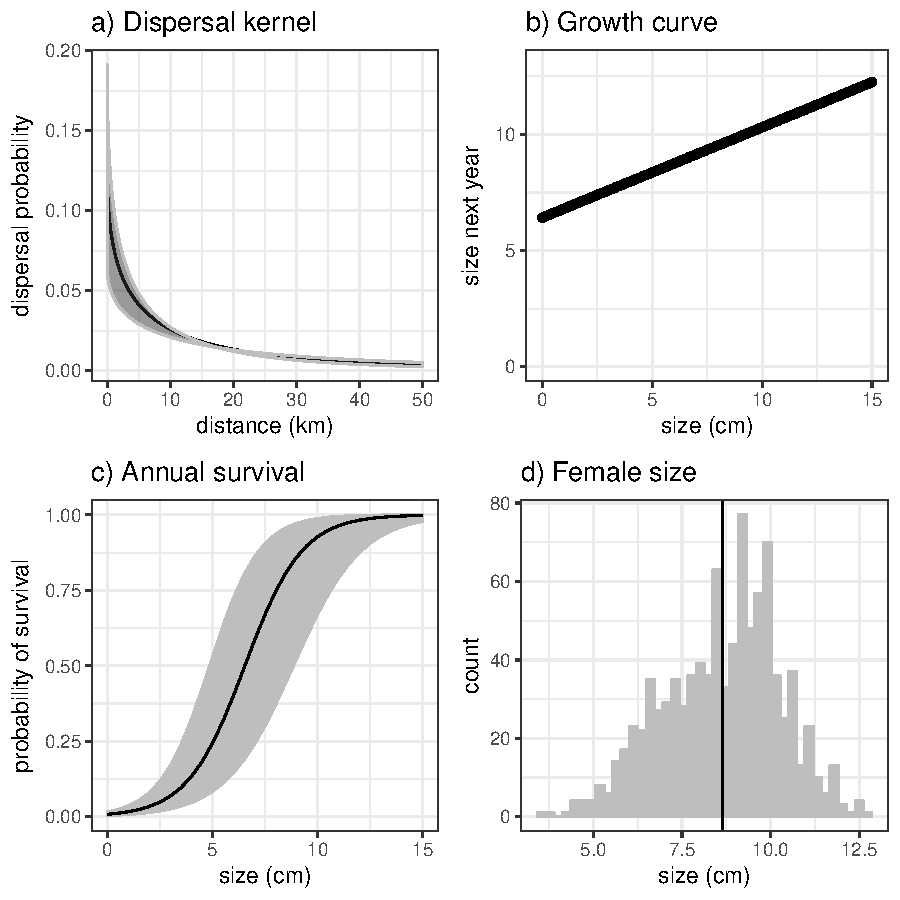
\includegraphics[width = 1.0\textwidth]{\detokenize{../Plots/FigureDrafts/Parameter_inputs.pdf}}
	\caption{Best estimates (solid black line) and uncertainty (grey) for a) dispersal, b), growth, including the 1:1 line in thick black, c) post-recruit annual survival at Palanas as an example patch, and d) size at female transition parameters. \label{FIG_ParameterInputs}}
\end{figure}

% Figure 4 - abudance trends, LEP, LRP, local replacement metrics
\begin{figure}[H] % abudance trends and LEP, LRP LRP_local shown with uncertainty, line for best estimate (using mean offspring size as recruit size)
	\centering
	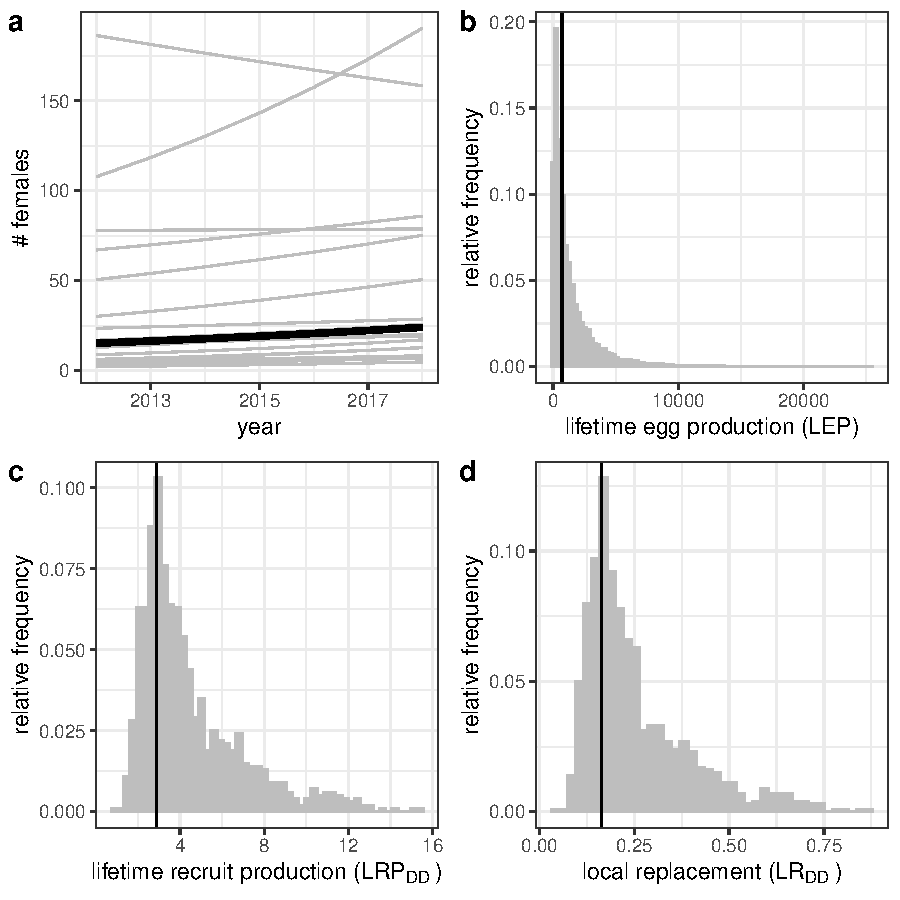
\includegraphics[width = 1.0\textwidth]{\detokenize{../Plots/FigureDrafts/Abundance_LEP_LRP_LocalReplacement_FreqPlots.pdf}}
	\caption{Estimates of a) estimated abundance of females over time at each individual patch (grey lines) and for an average patch (black line), b) individual-patch $\text{LEP}_i$ for all patches with the best estimate averaged across patches (black line), c) average LRP across patches, and d) local replacement, showing the best estimate (black solid line) and range of estimates considering uncertainty in the inputs (grey). Estimates of LRP and LR include compensation for density-dependent mortality in early life stages. \label{FIG_Abun_LEP_LRP_LocalReplacement}}
\end{figure}

% % Old SP figure
% \begin{figure}[H] % SP with line for best estimate (using mean offspring size as recruit size)
% 	\centering
% 	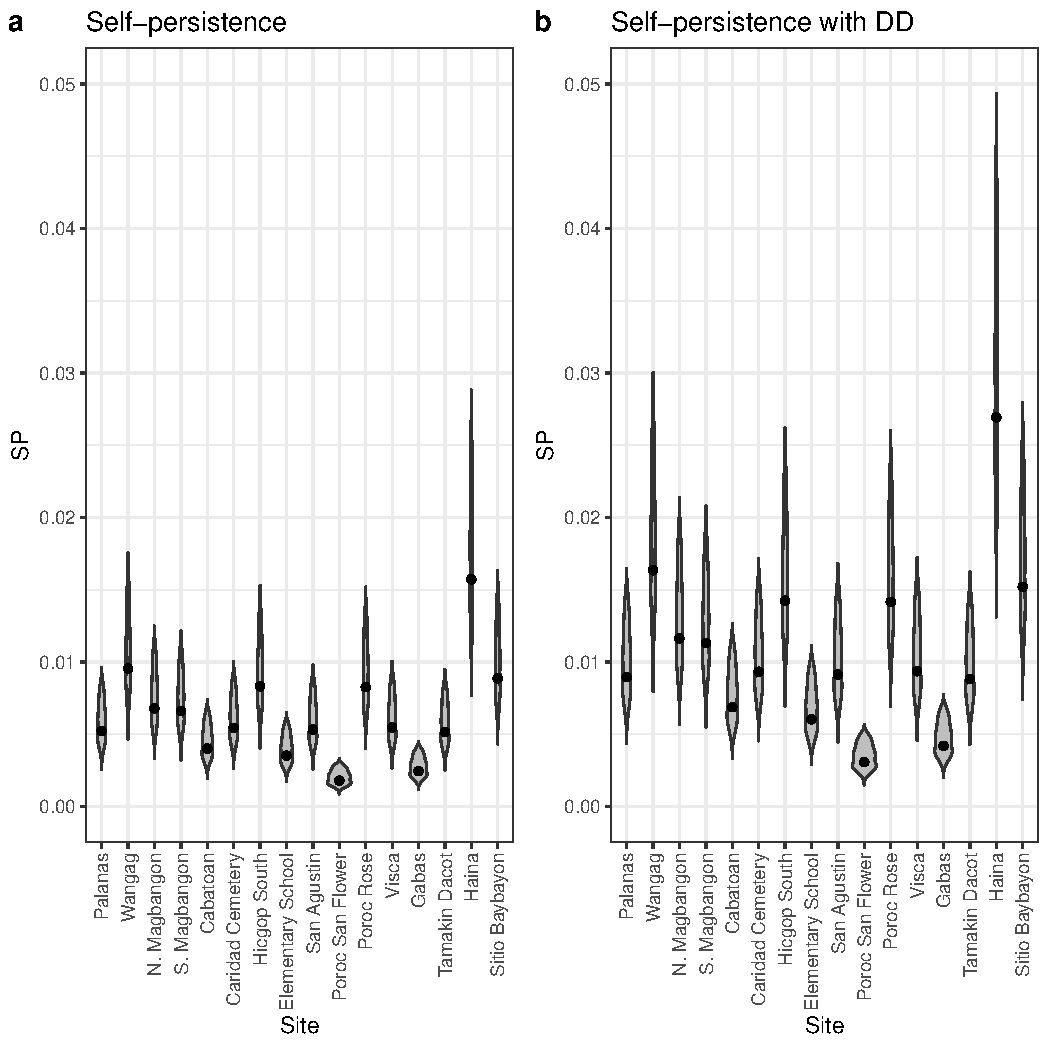
\includegraphics[width = 1.0\textwidth]{\detokenize{../Plots/FigureDrafts/SP_hists_by_site_noSLSTCP.pdf}}
% 	\caption{Values of self-persistence at each site, showing the best estimate (black point) and range of estimates considering uncertainty in the input paramters. No site reaches the value SP $\geq$ 1 necessary to be self-persistent. The estimates in (b) attempt to compensate for density-dependence in early life stages in our data, while the estimates in (a) do not. \label{FIG_SP}}
% \end{figure}

% Figure 5 - SP, realized connectivity matrix, and NP
\begin{figure}[H] % NP with line for best estimate (using mean offspring size as recruit size), realized connectivity matrix for best estimate - should re-do without Sitio Lonas, Sitio Tugas, Caridad Proper!
	\centering
	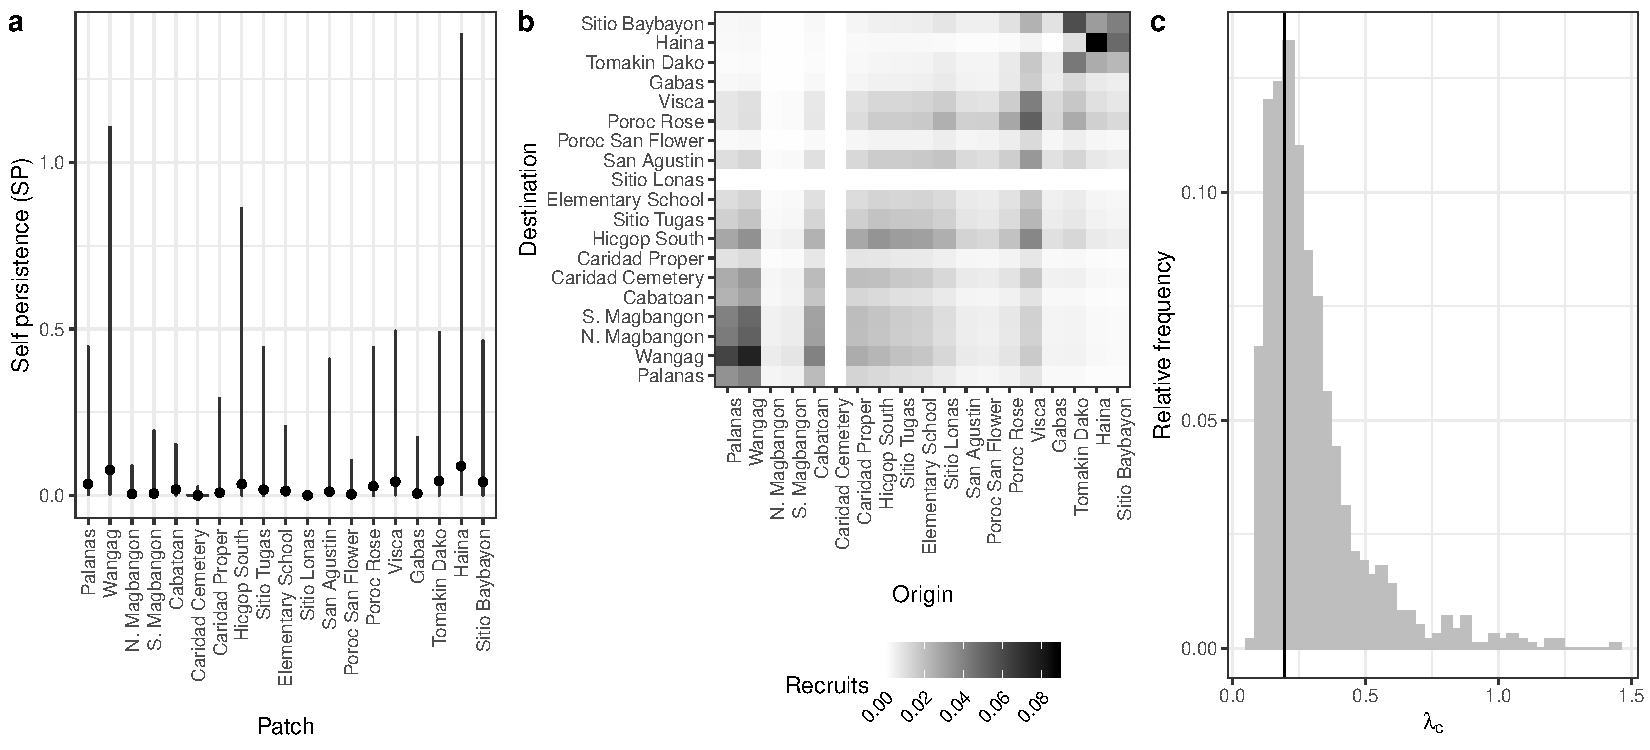
\includegraphics[width = 1.0\textwidth]{\detokenize{../Plots/FigureDrafts/SP_NP_connMatrixR_freq.pdf}}
	\caption{Values of a) self-persistence, b) realized connectivity among patches, and c) network persistence. All estimates include compensation for density-dependence in early life stages. For self-persistence (a) and network persistence (c), the best estimate is shown with in black (point for (a), line for (c)) and the range of estimates considering uncertainty is shown in grey. \label{FIG_SP_NP_realizedCmat}}
\end{figure}

% Figure 6 - what-ifs
\begin{figure}[H] 
	\centering
	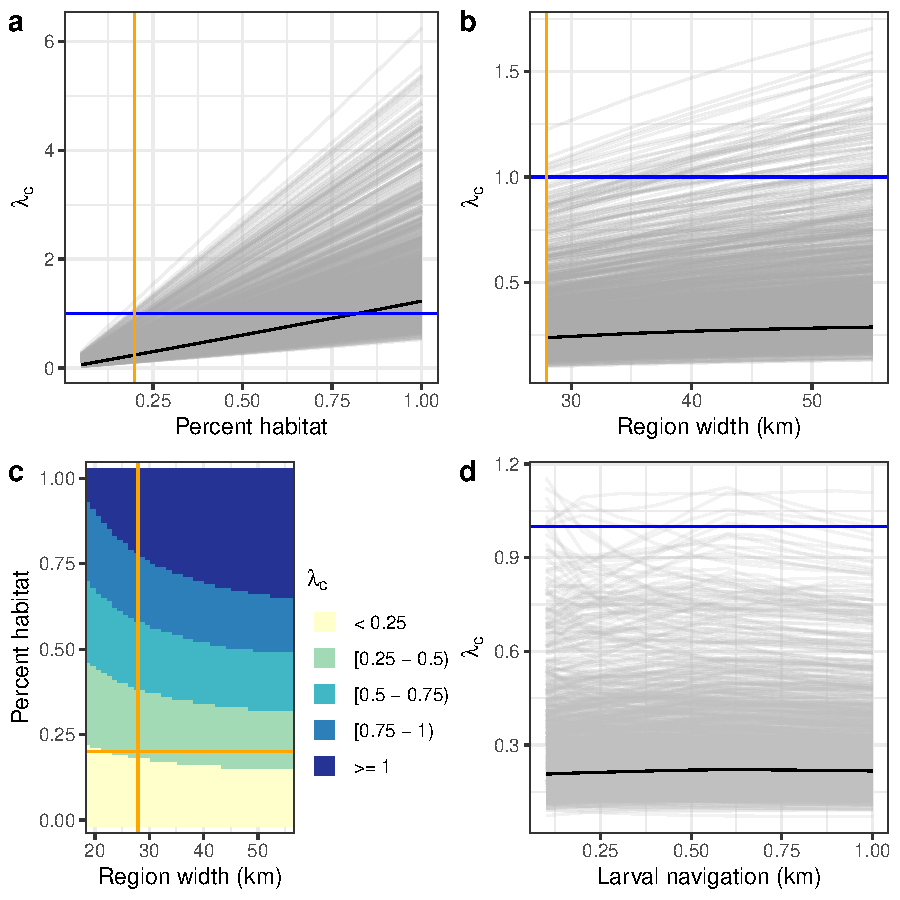
\includegraphics[width = 1.0\textwidth]{\detokenize{../Plots/FigureDrafts/What_if_4_panels_3D.pdf}}
	\caption{Sensitivity of network persistence to a) the proportion of the sampling region that is habitat, b) the width of the region maintaining the same proportion habitat (20\%), c) the width of the region when 100\% of the region is habitat, and d) larval navigation, where a buffer is added to the patch edges. Each metric calculation is a grey line and the best estimate is in black. The orange line shows the real proportion habitat and the blue line shows the persistence threshold. \label{FIG_WIs}}
\end{figure}
\newpage{}

{\LARGE Appendix}

% Hmm, they’re blank on my copy, too. I think one was about reformatting the table so that it was easier to read, perhaps including turning the page 90°, single-spacing, combining the best estimate and uncertainty columns (e.g., -2.33 [-2.81 to -1.22]), and using font size 11. The other comment was probably about creating one supplement, ordered into Supplemental Methods, Supplemental Results, Supplemental Tables, and Supplemental Figures.

\appendix

\renewcommand{\theequation}{A\arabic{equation}}
% redefine the command that creates the equation number.
\renewcommand{\thetable}{A\arabic{table}}
\setcounter{equation}{0}  % reset counter 
\setcounter{figure}{0}
\setcounter{table}{0}
\numberwithin{equation}{section}
\numberwithin{figure}{section}

\section{Supplemental Methods} \label{APP_SUPP_METHODS}
% Order in main text: theory (lifetime recruit production, self-persistence, network persistence, local replacement), parentage analysis/dispersal kernel, growth and survival (mark-recap), fecundity, lifetime egg production, survival from egg to recruit, density-dependence, estimated abuncance over time, exploring alternative geographies and larval navigation

\subsection{Defining recruit and census stage} \label{APP_SEC_METHODS_Recruit_def}

When assessing persistence, we must consider mortality and reproduction that occurs across the entire life cycle to determine whether an individual is replacing itself with an individual that reaches the same life stage \citep{burgess2014beyond}. We defined a recruit to be a juvenile individual that has settled on the reef within the previous year, which also encompasses the size we were first able to sample (3.5-6.0 cm for parentage studies) (Fig.\ \ref{FIG_Schematic}). In theory, it does not matter how we defined recruit as long as we used that definition in our calculations of both egg-recruit survival and LEP. In our system, however, while it is straightforward to calculate LEP from any size, we did not have enough tagged recruits to reliably estimate survival to different recruit sizes. Instead, we chose the mean size of offspring matched in the parentage study as our best estimate of the size of a recruit ($\text{size}_\text{recruit}$) and tested sensitivity to different recruit sizes by sampling from a uniform distribution over the sizes the recruit stage covers (3.5-6 cm, Table \ref{APP_TAB_Params}).

\subsection{Self persistence}

Our equation for SP is a modification of that used in \cite{burgess2014beyond}, which uses LEP to represent offspring produced and uses local retention (the number of surviving recruits that disperse back to the natal patch divided by the number of eggs produced by the natal patch) to capture egg-recruit survival and dispersal combined: LEP×local retention ≥ 1. We modify this to include egg-recruit survival in the offspring term instead, using LRP in place of LEP.

\subsection{Dispersal kernel} \label{APP_SEC_METHODS_Dispersal}

\subsection{Growth and survival} \label{APP_SEC_METHODS_Growth_and_survival}

To include size in the mark-recapture model for survival, we used the growth model (eqn.\ \ref{EQN_VBL}) and the size recorded or estimated in the previous year to estimate the size of fish not recaptured in a particular year. Fish are not well-mixed at our patches and divers needed to swim near an anemone to have a reasonable chance of capturing the fish on it so we also included a distance effect on recapture probability (Table \ref{APP_TAB_MARKmodels}). We used diver GPS tracks to estimate the minimum distance between a diver and the anemone where the fish was first caught for each tagged fish in each sample year.

We compared the fit of the models using a modified version of the Akaike information criterion that reduces the potential for overfitting with small sample sizes (AICc) and selected the model with the lowest AICc value (Table \ref{APP_TAB_MARKmodels}).

% Using diver GPS tracks, we estimated the minimum distance between a diver and the anemone for each tagged fish in each sample year to include as a factor. 

% From the mark-recapture analysis of tagged and genotyped fish, we estimate mean values of $L_\infty = 10.71 \text{cm}$ (range of estimates 10.50 - 10.90 cm) and $K = 0.864$ (range of estimates 0.785 - 0.944) for the von Bertalanffy growth curve parameters (eqn.\ \ref{EQN_VBL}, Fig.\ \ref{FIG_ParameterInputs}b, Table \ref{APP_TAB_Params}). For juvenile and adult (post-recruitment) survival on a log-odds scale, the best-fit model has an effect of size, with coefficient $b_a = 0.169 \pm 0.028$ SE and intercept $b_\phi = -1.83 \pm 0.231$ SE (eqn.\ \ref{EQN_Survival}). The accompanying best-fit model for log-odds recapture probability has a negative size effect and a negative effect of diver distance from the anemone (eqn.\ \ref{APP_EQN_MARKRecapture}, Fig.\ \ref{APP_FIG_RecapSizeDistEffect}).

% \subsection{Breeding size} \label{APP_SEC_METHODS_BreedingSize}

% We only considered reproduction during the female life stage of the fish. Fecundity was therefore 0 up to the size of transition from male to female ($L_f$) and then was size-dependent, described below (SI \ref{APP_SEC_METHODS_Fecundity}). We used the 

% We only considered reproductive effort once the fish is female and used the average size of first female observation for recaptured fish as the transition size $L_f = 9.32 \text{cm}$.

% We used the average size of the first female observation for recaptured fish as the estimate $L_f$, 
% For fish caught as both male and female, we used the size recorded when they were first captured as female (full data set shown in Fig.\ \ref{FIG_ParameterInputs}d). We used the mean of those sizes as our estimate of $L_f$ and randomly sampled from the full set with replacement to generate a distribution of sizes to use in our uncertainty calculations. 

\subsection{Fecundity} \label{APP_SEC_METHODS_Fecundity}

We used a size-dependent fecundity relationship determined using photos of egg clutches and females \citep{yawdoszynInPrepfecundity}, where the number of eggs per clutch ($E_c$) is exponentially related to the length in cm of the female ($L$) with size effect $\beta_l = 2.388$, intercept $b = 1.174$, and egg age effect $\beta_e = -0.608$ dependent on if the eggs were old enough to have visible eyes. For fish larger or equal to the transition to female size $L_f$, we multiplied the number of eyed eggs per clutch by the number of clutches per year $c_e = 11.9$ \citep[estimate from][]{holtswarth2017fecundity} to get total annual fecundity $f$ for a female of length $L$:

\begin{equation}
f(L) = 
\begin{cases}
0, & \text{if } L < L_f \\
c_e * e^{\beta_l\ln(L) + \beta_e[\text{eyed}] + b}, & L \geq L_f. \label{EQN_Fec}
\end{cases}
\end{equation}

% \begin{equation}
% f = c_e * e^{\beta_l\ln(L) + \beta_e[\text{eyed}] + b}. \label{EQN_Fec}
% \end{equation}

\subsection{Lifetime egg production (LEP)} \label{APP_SEC_METHODS_LEP}

To compute LEP, we discretized time and size (in eqn.\ \ref{EQN_LEP}) and summed across the matrix. When entering the starting individual into the matrix, we used 0.1 as the standard deviation of size to spread out the starting individual across size bins. To account for differences in growth rates across fish, we used the size determined by the growth curve (eqn.\ \ref{EQN_VBL}) as the mean along with an estimate of spread ($\text{size}_{sd}$) when projecting the size distribution of the fish in the next year. We used our recapture data to estimate the standard deviation ($\text{size}_{sd}$) of the distribution of sizes in the next year of fish starting from one size (Table \ref{APP_TAB_Params}). % Which size was that? Put the numbers of starting size and spread in here?

LEP was estimated by site because each patch has a different estimate of survival, represented as $\text{LEP}_i$. We also present the average LEP across patches, noted as $\text{LEP}_*$ (Fig.\ \ref{FIG_Abun_LEP_LRP_LocalReplacement}b) and used to estimate average LRP and LR for the metapopulation (Fig.\ \ref{FIG_Abun_LEP_LRP_LocalReplacement}c, d). 

To estimate egg-recruit survival ($S_e$), we used the expected lifetime egg production for a fish that has already survived to reach parent size (6.0 cm) so $L_s$ in eqn.\ \ref{EQN_LEP} = 6.0, rather than 3.5. We used the average LEP for parent-sized fish across patches, noted as $\text{LEP}_p$.
% To compute LEP, we discretize time and size and sum across the matrix. When entering the starting individual into the matrix, we use 0.1 as the standard deviation of size to spread the starting individual across size bins ($\text{size}_{\text{recruit}, sd}$). When projecting the distribution of the size of the fish in the next year, we used the growth curve (eqn.\ \ref{EQN_VBL}) to find the mean and an estimate from our recapture data of the standard deviation ($\text{size}_{sd}$) of the distribution of sizes in the next year of fish starting from one size (\ref{APP_TAB_Params}). % EDIT THIS TO MAKE MORE SENSE! MAYBE WILL's COMMENTS WILL HELP?

%We only considered reproductive effort once the fish is female and used the average size of first female observation for recaptured fish as the transition size $L_f = 9.32 \text{cm}$.

\subsection{Alternate geographies and larval navigation}

\paragraph{Larval navigation} \label{APP_SEC_METHODS_Larval_nav}

In our sensitivity test to larval navigation and swimming, we added a buffer represenging navigation ranging from 0 - 1 km to the edges of the destination patches when determining probability of dispersal between patches. To avoid the shadows of effective patch area from overlapping, we added no more than half the distance between two adjacent patches to each patch. The buffers changed the proportion of the sampling region that is habitat (\ref{APP_SEC_PropHabInSampledRegion}), as we considered the buffer areas to be habitat as well, which affected the scaling of recruits in egg-recruit survival.

\subsection{Scaling up recruits} \label{APP_SEC_METHODS_ScalingUpRecruits}

To estimate the total number of offspring produced by genotyped parents that survived to recruitment, we scaled up the number of matched offspring caught during sampling ($R_m$) to account for recruits we could have missed (Fig.\ \ref{APP_FIG_RecruitScalingSchematic}). We scaled up by 1) the cumulative proportion of habitat we sampled at our patches over time ($P_h$) to account for recruits at anemones we did not sample (details in \ref{APP_SEC_ProbHabSampled}), 2) the probability of capturing a fish if we sampled its anemone ($P_c$) to account for fish that escaped during sampling (details in \ref{APP_SEC_ProbR}), 3) the proportion of the dispersal kernel from our patches covered within our sampling region ($P_d$) to account for fish that dispersed outside of our sampling area (details in \ref{APP_SEC_PropDispKernelSampled}), and 4) the proportion of our sampling region that was habitat ($P_s$) to avoid counting mortality of fish dispersing to non-habitat within our region twice (in both the estimate of total recruits and in the integrated dispersal kernel) (details in \ref{APP_SEC_PropHabInSampledRegion}). %, and 5) the proportion of anemones occupied by \textit{A. clarkii} ($DD$) to account for density-dependent mortality of settling recruits.

\paragraph{Proportion of habitat sampled} \label{APP_SEC_ProbHabSampled}

We used tagged anemones to estimate the proportion of habitat we sampled within our patches. We tagged each anemone that was home to yellowtail anemonefish with a metal tag, which is relatively permanent and easy to re-sight (the anemone tag is visible above the anemone in Fig.\ \ref{FIG_Map_and_photo}c). We therefore considered the total number of metal-tagged anemones at a patch to be the habitat present. We used proportion of anemones rather than proportion of total patch area because anemones, and therefore habitat quality, were unevenly distributed across each patch; areas we did not visit likely had a lower anemone density than the areas we did sample. % We divided the number of tagged anemones visited each sampling year by the total number of metal tags at that patch to get the proportion of habitat sampled. We used tagged anemones to estimate the proportion of habitat we sampled at each patch in each year ($P_{h_{i,t}}$).

To scale the number of tagged recruited offspring to account for areas of our patches we did not sample, we used the overall proportion habitat sampled across all patches and sampling years ($P_h$). We summed the metal-tagged anemones we visited across all patches and years, then divided by the number of anemones we could have sampled (the sum of total metal-tagged anemones across all patches multiplied by the number of sampling years).

\paragraph{Probability of capturing a fish, from recapture dives} \label{APP_SEC_ProbR}

To estimate the probability of capturing a fish given that we sampled its anemone ($P_c$), we used mark-recapture data from recapture dives done within a sampling season. During some of the sampling years, portions of the patches were sampled again within a few weeks of the original sampling dives. We assumed that the probability of recapturing a fish on a recapture dive was the same as capturing a fish on a sampling dive, assuming there was no mortality in the weeks between dives and that the fish did not alter their behavior towards divers. For each recapture dive, we used GPS tracks of the divers to identify the anemones covered in the recapture dive and the set of PIT-tagged fish encountered on those anemones during the original sampling dives. We estimated the probability of capture $P_c$ as the number of tagged fish re-caught during the capture dive $m_2$ divided by the total number of fish caught on the recapture dive $n_2$: $P_c = \frac{m_2}{n_2}$. %The value of $P_c$ from each recapture dive is reported in Table \ref{APP_TAB_RecapDives}. CHECK THIS AND REWORD!!!

We used the mean $P_c$ across all 14 recapture dives, covering XX patches in 3 sampling seasons (2016, 2017, 2018), as our best estimate. To consider uncertainty in $P_c$, we represented the probability of capture as a beta distribution, using the mean $\mu_{P_c}$ and variance $V_{P_c}$ of the set of 14 values to find the appropriate $\alpha_{P_c}$ and $\beta_{P_c}$ parameters, where 

\begin{eqnarray}
\alpha_{P_c} &=& (\frac{1-\mu_{P_c}}{V_{P_c}} - \frac{1}{\mu_{P_c}}) \mu_{P_c}^2 \\
\beta_{P_c} &=& \alpha_{\mu_{P_c}} \times \frac{1}{\mu_{P_c} - 1}. \label{APP_EQN_ProbCapBetaDistParams}  % Should I cite a source for this?
\end{eqnarray}

% Should I include a table of the recapture probs for each recapture dive, including site and year?
The mean of the individual capture probability values was $\mu_{P_c} = 0.56$, with variance $V_{P_c} = 0.069$, giving beta distribution parameters $\alpha_{P_c} = 1.44$ and $\beta_{P_c} = 1.13$. We sampled 1000 values from the beta distribution, then truncated the sample to include only values larger than the lowest value of $P_c$ estimated from an individual dive (0.20), to avoid unrealistically low values randomly sampled from the distribution. We then sampled with replacement from the truncated set to get a vector of 1000 values.

\paragraph{Proportion of dispersal kernel area sampled} \label{APP_SEC_PropDispKernelSampled}

To account for recruits that dispersed outside our sampling region, we found the proportion of the dispersal kernels from all parents that fell within our sampling region. For each of the nineteen patches, we found the area under the kernel ($A_i$) from the center of the patch to the north edge of the sampling area ($d_N$) (northern-most tagged anemone at Palanas, the northern-most patch) and the center of the patch to the south edge of the sampling area ($d_S$) (southern-most tagged anemone at Sitio Baybayon, the southern-most patch), then multiplied by the number of genotyped parents at that patch ($N_{g_i}$). We added the areas together, then divided by the sum of the total area under the dispersal kernel in both directions (1 when the kernel was normalized to 0.5) multiplied by the total number of genotyped parents ($N_g$) to get the proportion of the total dispersal kernel area covered by our sampling region ($P_d$):

\begin{equation} 
%p_{A, B}(d) = \int_{d_1}^{d_2} e^k e^{-(e^k d)^\theta}  dd. \label{EQN_integratingDK}
A_i = N_{g_i} \left( \int_{0}^{d_N} z e^{-(zd)^\theta}  dd + \int_{0}^{d_S} z e^{-(zd)^\theta}  dd \right), \label{EQN_DK_area_within_sampling_region}
\end{equation}

\begin{equation}
P_d = \frac{\sum_{i=1}^{19} A_i}{N_g}.
\end{equation}

\paragraph{Proportion habitat in sampling area} \label{APP_SEC_PropHabInSampledRegion}

To avoid counting mortality due to larvae settling on non-habitat twice - once in scaling up our matched recruits, which only included those who settled on habitat, and once in integrating the dispersal kernel - we scaled the estimate of total surviving recruits from our patches by the proportion of our sampling region that was habitat ($P_s$). We found $P_s$ by summing the lengths of all the patches, which run approximately north-south, and dividing by the total north-south distance of our sampling region, giving $P_s = 0.20$. We assumed that larvae were unable to navigate to habitat if they dispersed to an unsuitable area but relaxed that assumption in our sensitivity tests (\ref{APP_SEC_METHODS_Larval_nav}) as anemonefish larvae do likely have some ability both to sense good settlement areas, either by detecting host anemones \citep{elliott1995host, arvedlund1999host} or conspecifics \citep[e.g.][for coral reef fish more broadly]{lecchini2005experimental}, and to swim in a particular direction \citep[e.g.][]{bellwood2001relative, fisher2005swimming}.


\subsection{Characterizing uncertainty} \label{APP_SEC_Uncertainty}

\paragraph{Dispersal kernel} \label{APP_SEC_Uncertainty_Dispersal}

To account for uncertainty in the dispersal kernel, we used sets of the shape parameter $\theta$ and the scale parameter $k_d$ that represented the span of the 95\%confidence interval when $k_d$ and $\theta$ were estimated jointly \citep[Table \ref{APP_TAB_Params},][]{catalanoInPrepconnectivity}. We randomly sampled pairs of $\theta$ and $k_d$ parameters from the distribution, weighted by the log-likelihood.

\paragraph{Growth} \label{APP_SEC_Uncertainty_Growth}

We used the first and second capture lengths for fish that were recaught after a year (within 345 to 385 days) to estimate L∞ and K (using eqn.\ \ref{EQN_VBL}). For fish recaptured more than once, we randomly selected only one recapture period from each to use to estimate the von Bertalanffy parameters and repeated the random selection and estimate 1000 times. We found the mean estimates (L∞ = 10.70 cm, K = 0.864) and mean standard error of those fits, then sampled from within that range to generate a set of von Bertalanffy growth curves to use in our LEP calculations (Fig. 2b, Table A1).

\paragraph{Survival} \label{APP_SEC_Uncertainty_Survival}

\paragraph{Size of transition to female} \label{APP_SEC_Uncertainty_FemaleSize}

 To incorporate uncertainty in the size at which male fish transition to female (and reproductive output is counted in eqn.\ \ref{EQN_LEP}), we sampled directly from the sizes at which recaptured fish were first captured as female (5.2 cm - 12.7 cm) (Fig.\ \ref{FIG_ParameterInputs}d).

\paragraph{Lifetime Egg Production (LEP)} \label{APP_SEC_Uncertainty_LEP}

\paragraph{Egg-recruit survival} \label{APP_SEC_Uncertainty_Egg-recruit-surv}

We considered uncertainty in the number of offspring assigned to parents ($R_m$) and in the probability of capturing a fish ($P_c$). We generated a set of values for the number of assigned offspring using a random binomial, with the number of genotyped offspring (745) as the number of trials and the assignment rate from the parentage analysis (0.079) as the probability of success on each trial \citep{catalanoInPrepconnectivity}. For the probability of capturing a fish, we sampled values from a beta distribution that captured the mean and variance of capture probabilities across recapture dives (details in \ref{APP_EQN_ProbCapBetaDistParams}).

\newpage{}{}

\section{Supplemental Results}  %%% STILL NEED TO REARRANGE ORDER TO MATCH MAIN TEXT!

\subsection{Parentage} \label{APP_SEC_RESULTS_Parentage}

From the genetic work and parentage analysis done in \cite{catalanoInPrepconnectivity}, we genotyped 1729 potential parents, genotyped 791 potential offspring, and matched 71 offspring to parents.

\subsection{Growth} \label{APP_SEC_RESULTS_Growth}

From the mark-recapture analysis of tagged and genotyped fish, we estimated mean values of $L_\infty = 10.70$ cm (with uncertainty bounds 9.81-11.65) and $K = 0.864$ (0.80-0.91) for the von Bertalanffy growth curve parameters (eqn.\ \ref{EQN_VBL}, Fig.\ \ref{FIG_ParameterInputs}b, Table \ref{APP_TAB_Params}). 

\subsection{Survival} \label{APP_SEC_RESULTS_Survival}

The best model for post-recruitment annual survival $\phi$ on a log-odds scale had a positive size effect ($b_a = 0.15 \pm 0.029$ SE) with intercepts $b_{\phi_i}$ varying by patch (eqn.\ \ref{APP_EQN_Survival}, Fig.\ \ref{APP_FIG_SurvBySizeAndSite}). The accompanying best model for recapture probability $p_r$ on a log-odds scale had a negative effect of size ($b_1 = -0.16 \pm 0.09$ SE) and a negative effect of diver distance from anemone ($b_2 = -0.15 \pm 0.02$ SE), with intercept $b_{p_r} = 2.14 \pm 0.87$ SE (eqn.\ \ref{APP_EQN_MARK_Recapture}, Fig.\ \ref{APP_FIG_RecapSizeDistEffect}). This suggests divers were less likely to recapture larger fish, which are stronger swimmers and more likely to flee when divers approach, and those at anemones far from areas sampled:

\begin{equation}
\log(\frac{\phi}{1-\phi}) = b_{\phi_i} + b_a\text{size}. \label{APP_EQN_Survival}
\end{equation}

\begin{equation}
\log(\frac{p_r}{1-p_r}) = b_{p_r} + b_1\text{size} + b_2d. \label{APP_EQN_MARK_Recapture}
\end{equation}

\subsection{Lifetime egg production (LEP)} \label{APP_SEC_RESULTS_LEP}
% For our persistence metrics, we present the estimate using the demographic and connectivity input values without uncertainty (the mean of the uncertainty distributions, with the exception of the size range for recruit), as the best estimate and the range with uncertainty shown in brackets. Using our best estimates for growth, survival, and fecundity, w
We calculated an average value of LEP across patches of 721 eggs with uncertainty bounds [82, 31657] (Fig.\ \ref{FIG_Abun_LEP_LRP_LocalReplacement}b), with best estimate values at individual patches that ranged from 0 to 1754 eggs. Uncertainty in adult survival had the largest effect on LEP (Fig.\ \ref{APP_FIG_Uncertainty_LEP}), which corresponds to longer-surviving individuals having more opportunities to reproduce at larger sizes. 

\subsection{Egg-recruit survival ($S_e$)} \label{APP_SEC_RESULTS_Egg-recruit_survival}

We estimated egg-recruit survival $S_{e}$ to be 0.002 [3.5e-05, 0.014] when we corrected for density-dependence in our data. Uncertainty in the size of transition to breeding female $L_f$ had the largest effect on egg-recruit survival (Fig.\ \ref{APP_FIG_Uncertainty_RperE}); the larger the transition size to female, the fewer tagged eggs we estimated were produced by our genotyped parents and the higher the estimate of egg-recruit survival. This differs from our finding above that adult survival had the largest effect on LEP because the starting size of the individual considered is lower when we estimate LEP for a recruit (4.37 cm, 3.5-6.0cm range) than for a parent (6.0cm). Fish considered parents in our parentage analysis have already survived one or more years since recruiting so the transition to breeding female plays a larger role in the number of eggs they are likely to produce than for fish who have just recruited. 

\subsection{Abundance trends by patch}

We used the number of females captured at each patch in each sampling year, scaled by the proportion of habitat sampled at that patch in that year and by the probability of capturing a fish, to estimate abundance trends for each patch (Fig.\ \ref{APP_FIG_AbundanceBySite}). Seventeen of the patches showed positive abundance trends (Fig.\ \ref{APP_FIG_AbundanceBySite}a-q), while the two southern-most patches showed declines (Haina and Sitio Baybayon, Fig.\ \ref{APP_FIG_AbundanceBySite}r,s).

\subsection{Persistence metrics without compensation for density-dependence} \label{APP_SEC_RESULTS_noDD} %NEED TO REPLACE THESE METRICS WITH THE UPDATED VALUES!!!
Estimating persistence metrics without compensating for density-dependence in our data gave us an understanding of whether individuals at our patches were able to replace themselves and whether our patches would persist in isolation at the current abundance levels, rather than at low abundance. Without compensation for early life density-dependence, all of our metrics showed that the set of patches we sampled is less likely to persist as an isolated network than the metrics for low abundance. We estimated egg-recruit survival ($S_e$) to be 0.0012 with uncertainty bounds [2.04e-05, 0.008] and average lifetime recruit production ($\text{LRP}$) across patches to be 0.84 [0.36, 4.54], with 55\% of LRP estimates $\geq 1$. (Fig.\ \ref{APP_FIG_LRP_LocalReplacement_noDD}c). Our estimate of local replacement (LR), which estimates replacement for recruits from our patches returning to our patches implictly including dispersal, was 0.10 [0.04, 0.52]. 

When we calculated LR using all arriving recruits to our patches, however, rather than just those originating there, the best estimate was $> 1$ (1.22, with 89\% of values with uncertainty $\geq 1$), suggesting that there was recruit-recruit replacement at our patches when we included immigrant recruits, even at current population levels when density-dependence was present.

We did not find any patches with a best estimate of SP $\geq 1$ or with uncertainty bounds that reached or exceeded 1 (Figs.\ \ref{APP_FIG_SP_NP_realizedCmat_noDD}a). Our best estimate of the dominant eigenvalue of the realized connectivity matrix $\lambda_c$ was 0.09 [0.04, 0.90] with 0\% of estimates where $\lambda \geq 1$ (Fig.\ \ref{APP_FIG_SP_NP_realizedCmat_noDD}c). 

\newpage{}

\section{Supplemental Tables}

\begingroup
\begin{landscape}
\singlespacing
\begin{longtable}{|p{1.0in}|p{1.5in}|p{1.5in}|p{1.25in}|p{1.0in}|p{1.5in}|}
\caption{Summary of parameter symbols, definitions, and values, including sections and equations where each are described in detail.} \label{APP_TAB_Params} \\ 
\hline
\textbf{Parameter} & \textbf{Description} & \textbf{Best estimate [uncertainty bounds]} & \textbf{Uncertainty origin} & \textbf{Details} & \textbf{Notes} \\ \hline
\multicolumn{6}{c|}{\textit{Dispersal and demographics}} \\ \hline
$K_d$ & scale parameter in dispersal kernel & \textbf{XX} & drawn from joint 95\% confidence limits with $\theta$, weighted by log-likelihood & eqn.\ \ref{EQN_integratingDK} & estimated in \cite{catalanoInPrepconnectivity}using methods in \cite{bode2018estimating} \\ \hline
$\theta$ & shape parameter in dispersal kernel & \textbf{XX} & drawn from joint 95\% confidence limits with $k_d$, weighted by log-likelihood &eqn.\ \ref{EQN_integratingDK} & estimated in \cite{catalanoInPrepconnectivity} using methods in \cite{bode2018estimating} \\ \hline
$L_\infty$ & average asymptotic size (cm) in von Bertalanffy growth curve & 10.70 cm \textbf{[]} & growth curve estimated with different pairs of fish & eqn.\ \ref{EQN_VBL} & \\ \hline
$k$ & growth coefficient in von Bertalanffy growth curve &  0.864 \textbf{[]} & \textbf{XX} & eqn.\ \ref{EQN_VBL} & \\ \hline 
\multicolumn{6}{c|}{\textit{Habitat and region characteristics}} \\ \hline
\multicolumn{6}{c|}{\textit{Alternate geographies and scenarios}} \\ \hline
\end{longtable}
\end{landscape}
\endgroup

% %[\textit{Need to clarify somewhere what kind of distributions are going into the uncertainty runs (drawn from data, uniform across a range, 95\% confidence bounds, etc.)}]
% % Make table prettier
% %%%% OLD VERSION OF TABLE - COMMENTING OUT PARAMETERS AS THEY GET DEALT WITH
% \begingroup
% \begin{landscape}
% \singlespacing
% \begin{longtable}{|p{1.1in}|p{1.5in}|p{1.5in}|p{1.8in}|}
% \caption{Summary of parameter symbols, definitions, and values.}\label{APP_TAB_Params} \\
% \hline 
% \textbf{Parameter} & \textbf{Description} & \textbf{Best estimate [uncertainty bounds]} & \textbf{Notes} \\ \hline
% $k_d$ & scale parameter in dispersal kernel & -2.33 [-2.81 to -1.22] & eqn.\ \ref{EQN_integratingDK}, estimated using methods in \cite{bode2018estimating} in Catalano et al.\ (in prep) \\ \hline
% $\theta$ & shape parameter in dispersal kernel & 1.19 [0.63 to 2.02] & eqn.\ \ref{EQN_integratingDK}, estimated using methods in \cite{bode2018estimating} in Catalano et al.\ (in prep) \\ \hline
% $L_\infty$ & average asymptotic size (cm) in von Bertalanffy growth curve & 10.70 cm [9.81 to 11.65] & eqn.\ \ref{EQN_VBL} \\ \hline
% $K$ & growth coefficient in von Bertalanffy growth curve &  0.864 [0.80 to 0.91] & eqn.\ \ref{EQN_VBL} \\ \hline  
% % $b_{\phi_{Cabatoan}}$ & intercept for adult survival at 0 cm at Cabatoan & -1.78 $\pm$ 0.33 standard error & on a log-odds scale, eqn.\ \ref{APP_EQN_Survival} \\ \hline 
% % $i_{\phi_{Cardidad Cemetery}}$ & addition to intercept for survival at Caridad Cemetery & -19.61 $\pm$ 2994 standard error & on a log-odds scale, eqn.\ \ref{APP_EQN_Survival} \\ \hline
% % $i_{\phi_{Elementary School}}$ & addition to intercept for survival at Elementary School & -0.11 $\pm$ 0.41 standard error & on a log-odds scale, eqn.\ \ref{APP_EQN_Survival} \\ \hline
% % $i_{\phi_{Gabas}}$ & addition to intercept for survival at Gabas & -0.42 $\pm$ 0.58 standard error & on a log-odds scale, eqn.\ \ref{APP_EQN_Survival} \\ \hline
% % $i_{\phi_{Haina}}$ & addition to intercept for survival at Haina & 0.12 $\pm$ 0.35 standard error & on a log-odds scale, eqn.\ \ref{APP_EQN_Survival} \\ \hline
% % $i_{\phi_{Hicgop South}}$ & addition to intercept for survival at Hicgop South & -0.06 $\pm$ 0.46 standard error & on a log-odds scale, eqn.\ \ref{APP_EQN_Survival} \\ \hline
% % $i_{\phi_{N. Magbangon}}$ & addition to intercept for survival at N. Magbangon & -1.31 $\pm$ 0.38 standard error & on a log-odds scale, eqn.\ \ref{APP_EQN_Survival} \\ \hline
% % $i_{\phi_{Palanas}}$ & addition to intercept for survival at Palanas & 0.24 $\pm$ 0.26 standard error & on a log-odds scale, eqn.\ \ref{APP_EQN_Survival} \\ \hline
% % $i_{\phi_{Poroc Rose}}$ & addition to intercept for survival at Poroc Rose & -0.19 $\pm$ 0.44 standard error & on a log-odds scale, eqn.\ \ref{APP_EQN_Survival} \\ \hline
% % $i_{\phi_{Poroc San Flower}}$ & addition to intercept for survival at Poroc San Flower & -0.52 $\pm$ 0.48 standard error & on a log-odds scale, eqn.\ \ref{APP_EQN_Survival} \\ \hline
% % $i_{\phi_{San Agustin}}$ & addition to intercept for survival at San Agustin & -0.47 $\pm$ 0.50 standard error & on a log-odds scale, eqn.\ \ref{APP_EQN_Survival} \\ \hline
% % $i_{\phi_{Sitio Baybayon}}$ & addition to intercept for survival at Sitio Baybayon & 0.02 $\pm$ 0.26 standard error & on a log-odds scale, eqn.\ \ref{APP_EQN_Survival} \\ \hline
% % $i_{\phi_{S. Magbangon}}$ & addition to intercept for survival at S. Magbangon & -1.08 $\pm$ 0.48 standard error & on a log-odds scale, eqn.\ \ref{APP_EQN_Survival} \\ \hline
% % $i_{\phi_{Tomakin Dako}}$ & addition to intercept for survival at Tomakin Dako & 0.39 $\pm$ 0.33 standard error & on a log-odds scale, eqn.\ \ref{APP_EQN_Survival} \\ \hline
% % $i_{\phi_{Visca}}$ & addition to intercept for survival at Visca & 0.33 $\pm$ 0.35 standard error & on a log-odds scale, eqn.\ \ref{APP_EQN_Survival} \\ \hline
% % $i_{\phi_{Wangag}}$ & addition to intercept for survival at Wangag & 0.35 $\pm$ 0.25 standard error & on a log-odds scale, eqn.\ \ref{APP_EQN_Survival} \\ \hline
% $b_a$ & size effect for adult survival & 0.15 $\pm$ 0.03 standard error & on a log-odds scale, eqn.\ \ref{APP_EQN_Survival} \\ \hline
% %$b_{p_r}$ & intercept for recapture probability from mark-recapture analysis & 2.10 & $\pm$ 0.849 standard error & on a log-odds scale, not used in persistence estimates \\ \hline
% %$b_1$ & size effect for recapture & -0.161 & $\pm$ 0.088 standard error & on a log-odds scale, not used in persistence estimates \\ \hline
% %$b_2$ & distance effect for recapture & -0.196 & $\pm$ 0.023 standard error & on a log-odds scale, not used in persistence estimates \\ \hline
% $\beta_e$ & coefficient for eyed eggs & -0.608 & eqn.\ \ref{EQN_Fec}, Yawdoszyn et al.\ (in prep) \\ \hline
% $\beta_l$ & size effect in eggs-per-clutch relationship & 2.39 & eqn.\ \ref{EQN_Fec}, Yawdoszyn et al.\ (in prep) \\ \hline
% $b$ & intercept in eggs-per-clutch relationship at female size 0 cm & 1.17 & eqn.\ \ref{EQN_Fec}, Yawdoszyn et al.\ (in prep) \\ \hline
% $c_e$ & egg clutches per year & 11.9 & eqn.\ \ref{EQN_Fec}, \cite{holtswarth2017fecundity} \\ \hline
% $\text{size}_\text{recruit}$ & size (cm) of recruited offspring & mean of size of offspring in parentage analysis = 4.37 cm [3.5 to 6.0 cm] & drawn from uniform distribution across range \\ \hline
% $\text{size}_{\text{recruit}, sd}$ & standard deviation of size of a recruit & 0.1 & used in discretization of IPM for LEP \\ \hline
% $\text{size}_{sd}$ & standard deviation distribution of sizes of a fish in the next year & 1.45 & used in discretization of IPM for LEP, estimated from range of sizes for fish starting at 7.4-7.6 cm and recaptured a year later \\ \hline
% $L_s$ & minimum size in LEP IPM & 0 cm & eqn.\ \ref{EQN_LEP} \\ \hline
% $U_s$ & maximum size in LEP IPM & 15 cm & eqn.\ \ref{EQN_LEP} \\ \hline
% %$S_e$ & egg-recruit survival & & &  \\ \hline
% %$E_c$ & eggs per clutch & depends on female size (eqn.\ \ref{EQN_Fec}) & & relationship from Yawdoszyn et al.\ (in prep) \\ \hline
% $L_f$ & size at transition to female & 9.32 cm [5.2 to 12.7 cm] & drawn from distribution in data \\ \hline
% $R_m$ & number of offspring matched to parents & 62	offspring & eqn.\ \ref{EQN_EggRecruitSurv} \\ \hline
% $N_g$ & number of genotyped parents & 1719 fish & eqn.\ \ref{EQN_EggRecruitSurv} \\ \hline
% $P_h$ & proportion of patches sampled cumulatively across time & 0.41 & eqn.\ \ref{EQN_EggRecruitSurv}, details in \ref{APP_SEC_ProbHabSampled} \\ \hline
% $P_d$ & proportion of dispersal kernel area from each patch covered by our sampling region & 0.57 & eqn.\ \ref{EQN_EggRecruitSurv}, details in \ref{APP_SEC_PropDispKernelSampled} \\ \hline 
% $P_c$ & probability of capturing a fish & 0.56 [drawn from beta distribution with parameters $\alpha_{P_c} = 1.44$ and $\beta_{P_c} = 1.13$] & eqn.\ \ref{EQN_EggRecruitSurv}, details in \ref{APP_SEC_ProbR} \\ \hline
% $P_s$ & proportion of our sampling region that is habitat & 0.20 & eqn.\ \ref{EQN_EggRecruitSurv}, details in \ref{APP_SEC_PropHabInSampledRegion} \\ \hline
% $\text{DD}$ & proportion of habitat that would be available without density-dependence at settlement & 1.71 & eqn.\ \ref{EQN_EggRecruitSurv} \\ \hline
% $p_U$ & proportion of anemones unoccupied by clownfish & 0.53 & used to estimate DD \\ \hline
% $p_A$ & proportion of anemones occupied by \textit{A. clarkii} & 0.38 & used to estimate DD \\ \hline
% \end{longtable}
% \end{landscape}
% \endgroup

%%%%% TABLE UPDATED (CREATED) 6/19/20
\begin{table}[!htbp] 
\begin{centering}
\caption{Table with site-specific survival ($\phi_i$) values on a log-odds scale (used in eqn.\ \ref{APP_EQN_Survival}), where the intercept is for adult survival for a fish of size 0 cm. The intercepts for each site is the intercept for Cabatoan plus the additional intercept value for that site, shown in the table.} \label{APP_TAB_SiteSurvivals}
\begin{tabular}{|p{1.1in}|p{0.75in}|p{0.75in}|p{1.25in}|p{1.5in}|}
\hline 
\textbf{Site} & \textbf{Intercept} & \textbf{Standard error} & \textbf{Confidence limits} & \textbf{Notes} \\ \hline
Cabatoan & -1.78 & 0.33 & -2.42 to -1.14 & \\ \hline
Caridad Cemetery & -19.66 & 0.00 & -19.66 to -19.66 & addition to Cabatoan intercept \\ \hline
Elementary School & -0.11 & 0.41 & -0.92 to 0.69 & addition to Cabatoan intercept \\ \hline
Gabas & -0.42 & 0.58 & -1.55 to 0.72 & addition to Cabatoan intercept \\ \hline
Haina & 0.12 & 0.35 & -0.57 to 0.81 & addition to Cabatoan intercept \\ \hline
Higcop South & -0.06 & 0.46 & -0.96 to 0.84 & addition to Cabatoan intercept \\ \hline
N. Magbangon & -1.31 & 0.38 & -2.05 to -0.57 & addition to Cabatoan intercept \\ \hline
Palanas & 0.24 & 0.26 & -0.26 to 0.75 & addition to Cabatoan intercept \\ \hline
Poroc Rose & -0.19 & 0.44 & -1.05 to 0.68 & addition to Cabatoan intercept \\ \hline
Poroc San Flower & -0.52 & 0.48 & -1.45 to 0.42 & addition to Cabatoan intercept \\ \hline
San Agustin & -0.47 & 0.50 & -1.45 to 0.42 & addition to Cabatoan intercept \\ \hline
Sitio Baybayon & 0.02 & 0.26 & -0.49 to 0.52 & addition to Cabatoan intercept \\ \hline
S. Magbangon & -1.08 & 0.48 & -2.02 to -0.14 & addition to Cabatoan intercept \\ \hline
Tomakin Dako & 0.39 & 0.33 & -0.25 to 1.03 & addition to Cabatoan intercept \\ \hline
Visca & 0.33 & 0.35 & -0.36 to 1.01 & addition to Cabatoan intercept \\ \hline
Wangag & 0.35 & 0.25 & -0.15 to 0.85 & addition to Cabatoan intercept \\ \hline
\end{tabular}
\end{centering}
\end{table}

%%%%% TABLE UPDATED 6/19/20 and comments in pdf addressed
\begin{table}[!htbp]
\begin{centering}
\caption{Table showing the set of models considered in MARK for survival ($\phi$) (from eqn.\ \ref{APP_EQN_Survival}) and recapture ($p_r$)  (from eqn.\ \ref{APP_EQN_MARK_Recapture}) probability, including effects of fish size ($S$), minimum distance from diver to the anemone where fish were first caught during surveys ($D$), year ($t$), and patch ($i$), and their relative AICc scores.}\label{APP_TAB_MARKmodels}
\begin{tabular}{|p{1.75in}|p{2.75in}|p{0.75in}|p{0.75in}|}
\hline 
\textbf{Model} & \textbf{Model description} & \textbf{AICc} & \textbf{dAICc} \\ \hline
$\phi \sim S+i$, $p_r \sim S+D$ & survival size+patch, recapture size+distance & 3104.1 & 0 \\ \hline
$\phi \sim i$, $p_r \sim S+D$ & survival patch, recapture size+distance & 3127.2 & -23.1 \\ \hline
$\phi \sim i$, $p_r \sim D$ & survival patch, recapture distance & 3127.2 & -23.1 \\ \hline
$\phi \sim S$, $p_r \sim S+D$ & survival size, recapture size+distance & 3139.9 & -35.8 \\ \hline
$\phi \sim S$, $p_r \sim D$ & survival size, recapture distance & 3141.6 & -37.5 \\ \hline
$\phi$, $p_r \sim S+D$ & survival constant, recapture size+distance & 3168.4 & -64.3 \\ \hline
$\phi$, $p_r \sim D$ & survival constant, recapture distance & 3169.3 & -65.2 \\ \hline
$\phi \sim t$, $p_r$ & survival time, recapture constant & 3243.9 & -139.8 \\ \hline
$\phi \sim i$, $p_r$ & survival patch, recapture constant & 3254.4 & -150.3 \\ \hline
$\phi$, $p_r \sim t$ & survival constant, recapture time & 3274.0 & -169.9 \\ \hline
$\phi \sim S$, $p_r \sim S$ & survival size, recapture size & 3345.1 & -241.0 \\ \hline
$\phi$, $p_r$ & survival constant, recapture constant & 3382.7 & -278.6 \\ \hline
\end{tabular}
\end{centering}
\end{table}

% Table updated 08 June 2020 (Caridad Proper, Sitio Lonas, Sitio Tugas all have 0 metal-tagged anems, 0 visited tagged anems in each year)
\begin{table}[!htbp]
\caption{Table showing the percent of anemones surveyed at each patch, ordered from north to south, in each sampling year.} \label{APP_TAB_PercHabSampled}
\begin{centering}
\begin{tabular}{|l|r|r|r|r|r|r|r|r|}
\hline 
\multicolumn{2}{|c|}{} & \multicolumn{7}{|c|}{\% Habitat surveyed} \\ \hline
Patch & \# Total anems & 2012 & 2013 & 2014 & 2015 & 2016 & 2017 & 2018 \\ \hline
Palanas & 138 & 29 & 57 & 48 & 61 & 85 & 86 & 86 \\ \hline  % changed
Wangag & 291 & 18 & 33 & 42 & 35 & 27 & 49 & 69 \\ \hline  % changed
N. Magbangon & 105 & 5 & 12 & 40 & 63 & 64 & 0 & 5 \\ \hline
S. Magbangon & 34 & 41 & 56 & 32 & 0 & 65 & 0 & 71 \\ \hline
Cabatoan & 26 & 42 & 58 & 58 & 65 & 73 & 0 & 62 \\ \hline
Caridad Cemetery & 4 & 0 & 75 & 50 & 0 & 50 & 50 & 50 \\ \hline
Caridad Proper & 4 & 0 & 100 & 0 & 0 & 0 & 0 & 0 \\ \hline  % all tagged anemones included in total anem estimate because there are no metal-tagged anems at this site
Hicgop South & 18 & 0 & 67 & 28 & 28 & 56 & 83 & 78 \\ \hline
Sitio Tugas & 8 & 0 & 100 & 0 & 0 & 0 & 0 & 0 \\ \hline  % all tagged anemones included in total anem estimate b/c no metal-tagged anems at this site
Elementary School & 7 & 0 & 100 & 43 & 100 & 100 & 86 & 100 \\ \hline  % changed
Sitio Lonas & 1 & 100 & 100 & 0 & 0 & 0 & 0 & 0 \\ \hline  % all tagged anems included in total anem estimate b/c no metal-tagged anems at this site
San Agustin & 18 & 89 & 61 & 72 & 61 & 100 & 89 & 72 \\ \hline  % changed
Poroc San Flower & 11 & 100 & 82 & 73 & 73 & 55 & 82 & 64 \\ \hline
Poroc Rose & 13 & 100 & 100 & 69 & 31 & 23 & 69 & 69 \\ \hline
Visca & 13 & 100 & 100 & 23 & 38 & 62 & 85 & 62 \\ \hline
Gabas & 9 & 0 & 0 & 0 & 44 & 44 & 67 & 0 \\ \hline
Tomakin Dako & 48 & 0 & 25 & 23 & 38 & 35 & 60 & 69 \\ \hline  % changed
Haina & 104 & 0 & 6 & 13 & 13 & 10 & 56 & 80 \\ \hline
Sitio Baybayon & 259 & 0 & 14 & 30 & 34 & 30 & 41 & 81 \\ \hline  % changed
Overall & 1111 & 16 & 32 & 36 & 39 & 42 & 48 & 67 \\ \hline
\end{tabular}
\end{centering}
\end{table}

% Table created 08 July 2020
\begin{table}[!htbp]
\caption{Table showing patch-specific estimates of lifetime egg production ($\text{LEP}_i$), lifetime recruit production ($\text{LRP}_i$), and self persistence ($\text{SP}_i$.)} \label{APP_TAB_PatchSpecificLEPandLRP}
\begin{centering}
\begin{tabular}{|l|r|r|r|}
\hline 
Patch & $\text{LEP}_i$ & $\text{LRP}_i$ & $\text{SP}_i$ \\ \hline
Palanas & 1383 & 2.91 & 0.017 \\ \hline  
Wangag & 1642 & 3.45 & 0.040 \\ \hline  
N. Magbangon & 133 & 0.28 & 0.002 \\ \hline
S. Magbangon & 183 & 0.39 & 0.003 \\ \hline
Cabatoan & 933 & 1.96 & 0.009 \\ \hline
Caridad Cemetery & 0 & 0 & 0 \\ \hline
Caridad Proper & 781 & 1.64 & 0.004 \\ \hline 
Hicgop South & 848 & 1.78 & 0.017 \\ \hline
Sitio Tugas & 781 & 1.64 & 0.003 \\ \hline  
Elementary School & 781 & 1.64 & 0.007 \\ \hline  
Sitio Lonas & 781 & 1.64 & 0 \\ \hline  
San Agustin & 445 & 0.92 & 0.006 \\ \hline  
Poroc San Flower & 415 & 0.87 & 0.002 \\ \hline
Poroc Rose & 694 & 1.46 & 0.014 \\ \hline
Visca & 1586 & 3.34 & 0.021 \\ \hline
Gabas & 483 & 1.02 & 0.003 \\ \hline
Tomakin Dako & 1760 & 3.70 & 0.022 \\ \hline  
Haina & 1130 & 2.38 & 0.044 \\ \hline
Sitio Baybayon & 959 & 2.02 & 0.021\\ \hline  
\end{tabular}
\end{centering}
\end{table}

% \textit{Talk to Katrina to fill out table with data that went into recapture calcs}

% \begin{table}[!htbp]
% \caption{Table showing the patch, year, number of fish caught on sample dives on the anemones resampled during the recapture dive ($m_2$), number of fish caught on the recapture dive ($n_2$) for each recapture dive.} \label{APP_TAB_RecapDives}
% \begin{centering}
% \begin{tabular}{|l|r|r|r|r|}
% \hline
% Patch & Year & $m_2$ & $n_2$ & $P_c$ \\ \hline
% & & & & 0.56 \\ \hline
% & & & & 0.26 \\ \hline
% & & & & 0.89 \\ \hline
% & & & & 0.67 \\ \hline
% & & & & 0.20 \\ \hline
% & & & & 0.83 \\ \hline
% & & & & 0.47 \\ \hline
% & & & & 0.20 \\ \hline
% & & & & 0.83 \\ \hline
% & & & & 1.0 \\ \hline
% & & & & 0.33 \\ \hline
% & & & & 0.58 \\ \hline
% & & & & 0.63 \\ \hline
% & & & & 0.41 \\ \hline
% \end{tabular}
% \end{centering}
% \end{table}

\newpage{}

\section{Supplemental Figures}

% NEED TO UPDATE THE EQUATION NUMBERS HERE!!
\begin{figure}[H] % Schematic
	\centering
	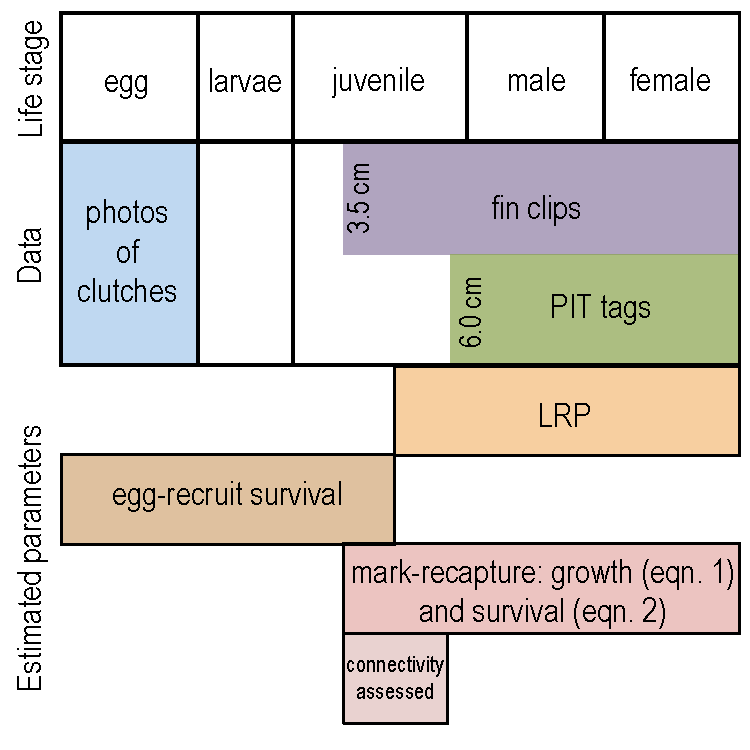
\includegraphics[width = 1.0\textwidth]{\detokenize{../Plots/Schematic/Schematic.pdf}}
	\caption{The data collected for fish at each life stage and how they match to the equations and metrics estimated. We considered recruits to be offspring in their first year of settlement, represented by the 3.5-6.0 cm range. \label{FIG_Schematic}} 
\end{figure}

\begin{figure}[!htbp] % Scaling up recruits
	\centering
	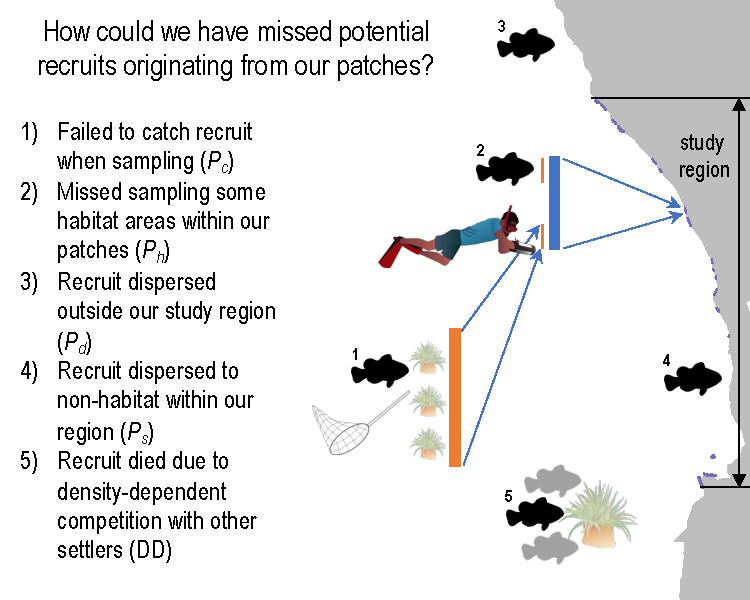
\includegraphics[width = 1.0\textwidth]{\detokenize{../Plots/UndercountingRecruits/RecruitScalingSchematic.pdf}}
	\caption{Schematic of five ways we could have missed recruits while sampling and used to scale up our raw estimate of recruits from matched offspring. \label{APP_FIG_RecruitScalingSchematic}}
\end{figure}

\begin{figure}[!htbp] % Range of parameter inputs for uncertainty runs
	\centering
	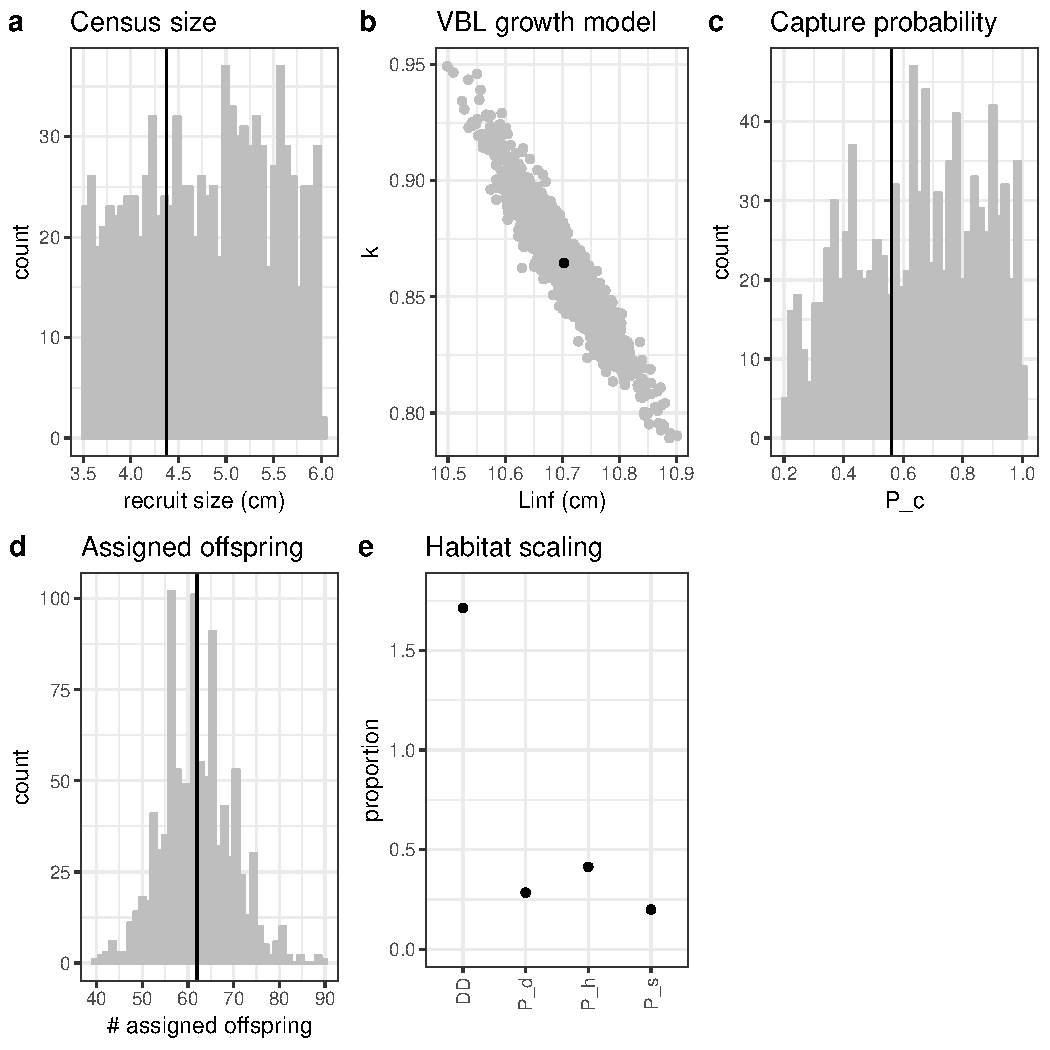
\includegraphics[width = 1.0\textwidth]{\detokenize{../Plots/FigureDrafts/APP_FIG_Parameter_inputs.pdf}}
	\caption{Range of parameter inputs for uncertainty runs with all uncertainty included, where the black line or point is the value used for the best estimate: a) $\text{size}_\text{recruit}$, the census size for recruits after egg-recruit survival; b) the parameters $L\infty$ and $K$ of the von Bertalanffy growth model; c) $P_c$, the probability of capturing a fish; d) number of offspring assigned back to parents in the parentage analysis; e) factors that scale the number of estimated recruits from our patch based on density-dependence in settler success (DD), proportion of the dispersal kernel captured by our sampling region ($P_d$), the cumulative proportion of our patches we sampled over time ($P_h$), and the proportion of our sampling area that was habitat ($P_s$). \label{APP_FIG_UncertaintyInputs}}
\end{figure}

\begin{figure}[!htbp] % Proportion of dispersal kernel area from each site sampled
	\centering
	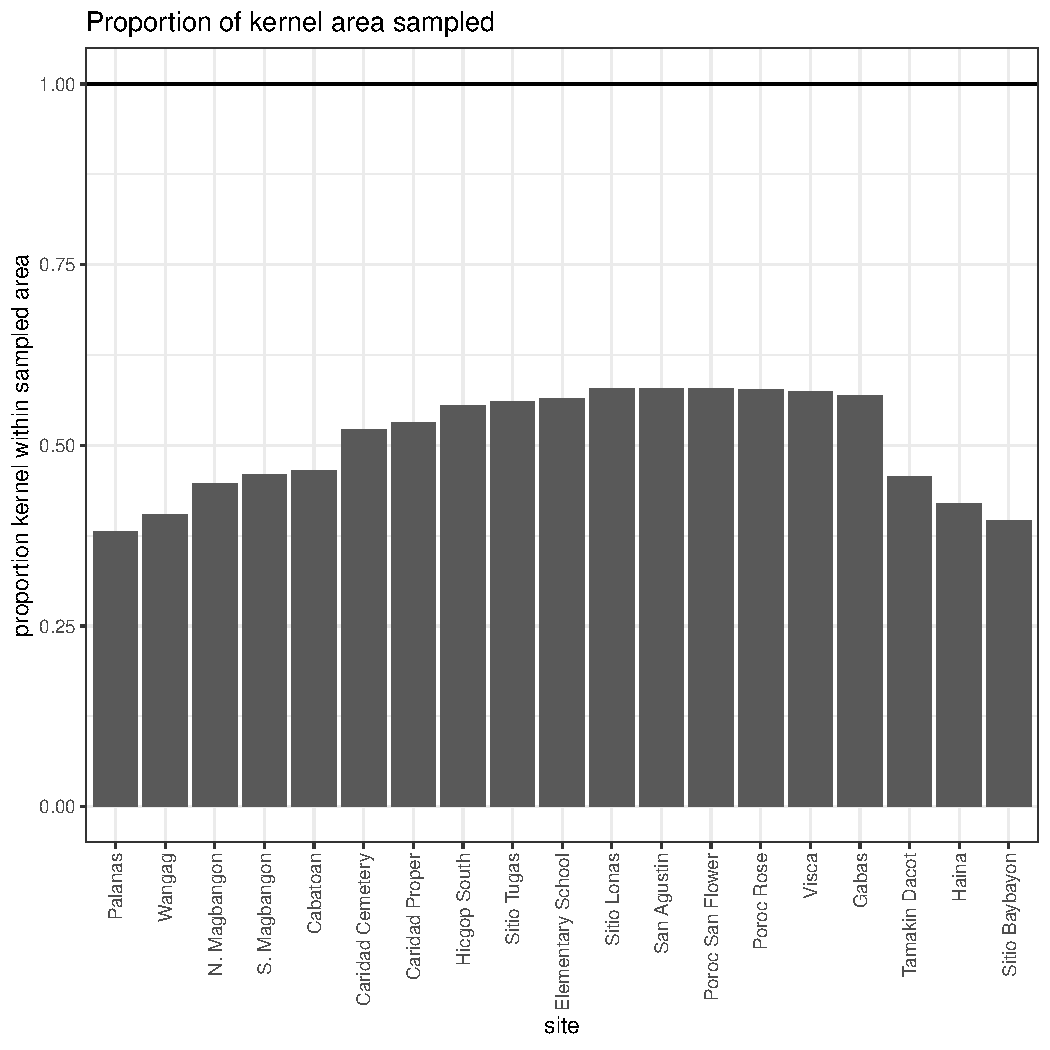
\includegraphics[width = 1.0\textwidth]{\detokenize{../Plots/FigureDrafts/Prop_of_kernel_area_sampled_by_site.pdf}}
	\caption{Proportion of the dispersal kernel area from the center of each patch covered by our sampling region. The overall proportion ($P_d$) is weighted by the number of parents at each patch. \label{APP_FIG_PropDispKernelAreaSampled}}
\end{figure}

\begin{figure}[!htbp] % site+size survival 
	\centering{}
	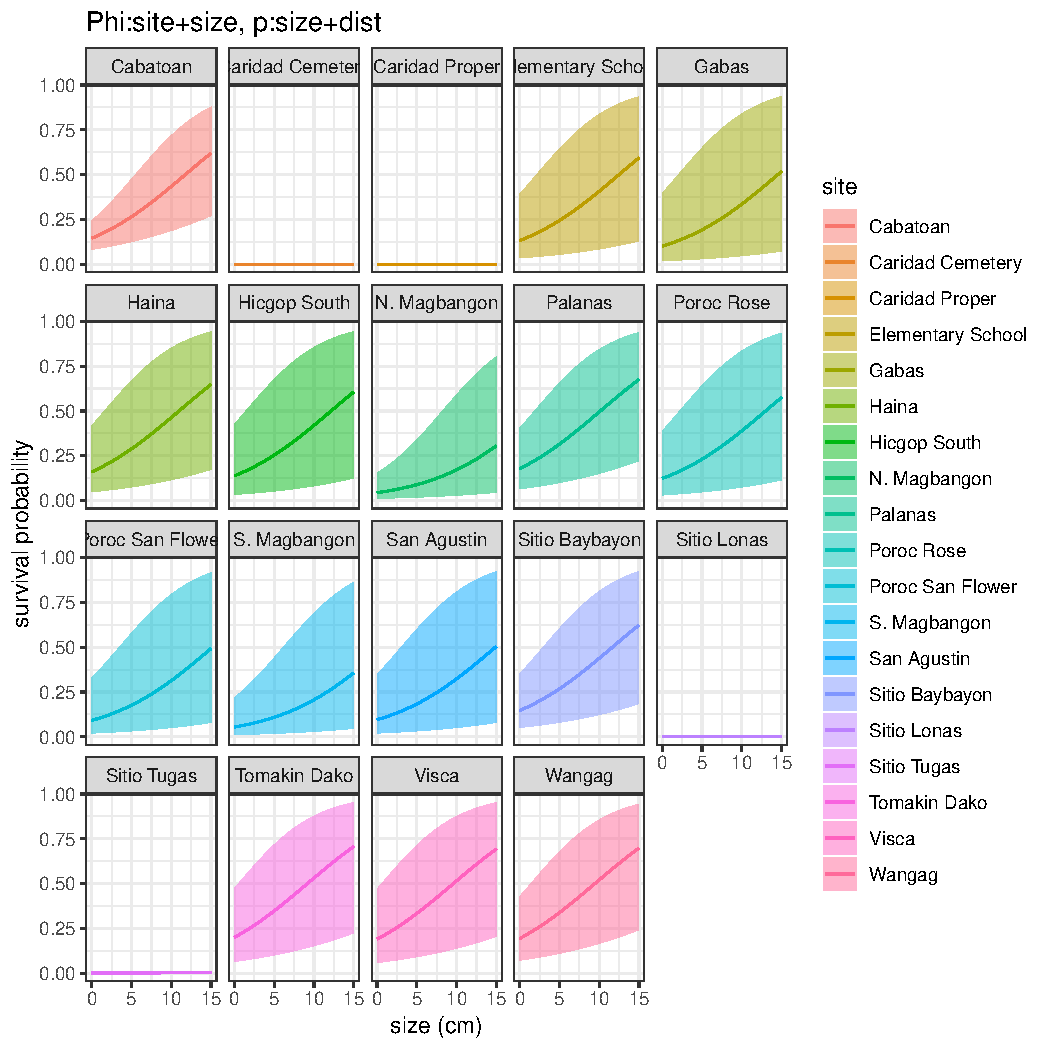
\includegraphics[width = 1.0\textwidth]{\detokenize{../Plots/FigureDrafts/APP_FIG_surv_by_size_and_site_Phisiteplussize_psizeplusdist.pdf}}
	\caption{Annual survival by size at each patch. \label{APP_FIG_SurvBySizeAndSite}}
\end{figure}

\begin{figure}[!htbp] % distance and fish size effects on recapture probability from MARK
	\centering
	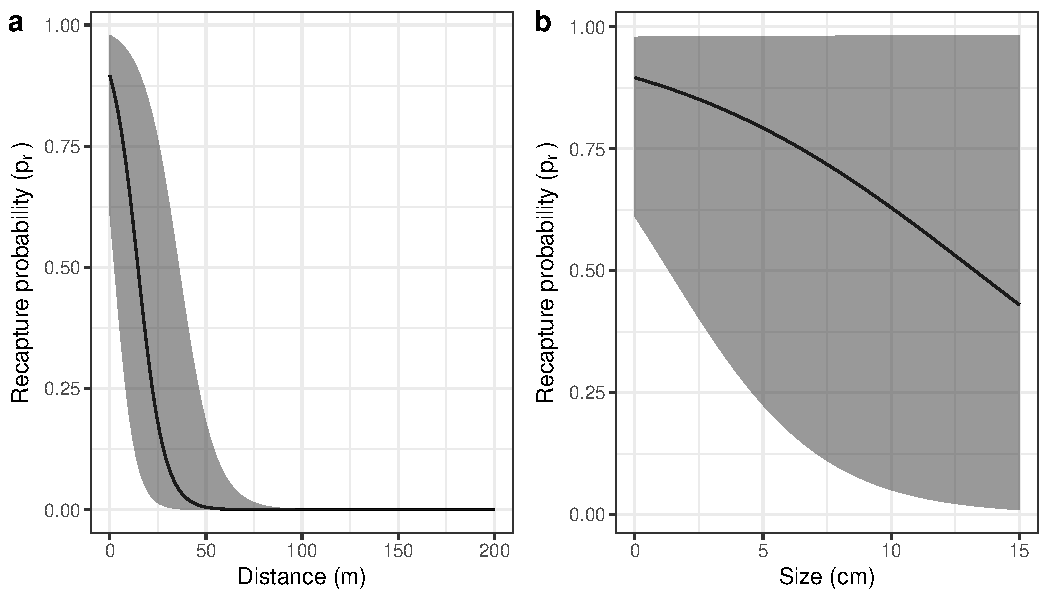
\includegraphics[width = 1.0\textwidth]{\detokenize{../Plots/FigureDrafts/APP_FIG_recap_effects_Phisiteplussize_psizeplusdist.pdf}}
	\caption{Effects of a) minimum distance between divers and the anemone where the fish was first caught and b) fish size on recapture probability, estimated along with survival in a mark-recapture analysis. \label{APP_FIG_RecapSizeDistEffect}}
\end{figure}

\begin{figure}[!htbp]  % Scaled estimates of females and trends by site
	\centering
	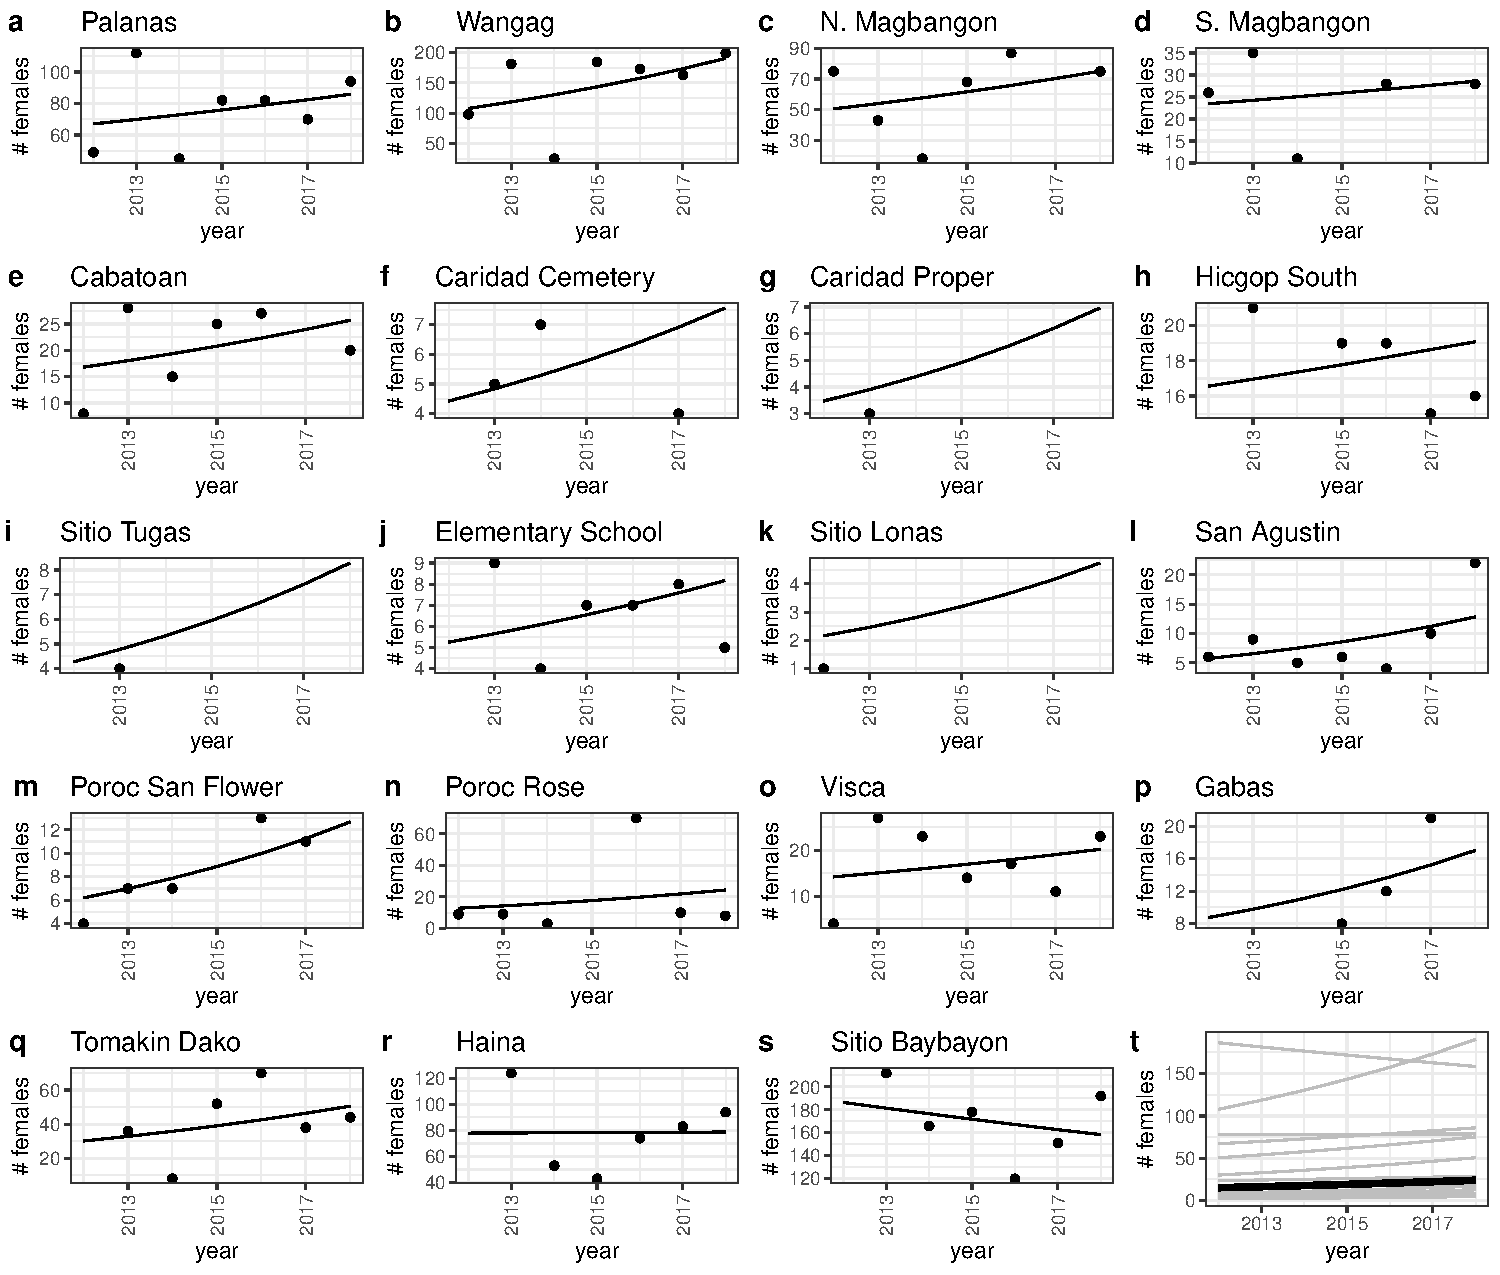
\includegraphics[width = 1.0\textwidth]{\detokenize{../Plots/FigureDrafts/Time_series_scaled_F_by_site_with_lines.pdf}}
	\caption{Scaled number of females captured (black dots) and abundance trends (black lines) by patch from a mixed effects model with patch as a random effect. \label{APP_FIG_AbundanceBySite}}
\end{figure}

\begin{figure}[!htbp] % LRP by site with DD compensation
	\centering
	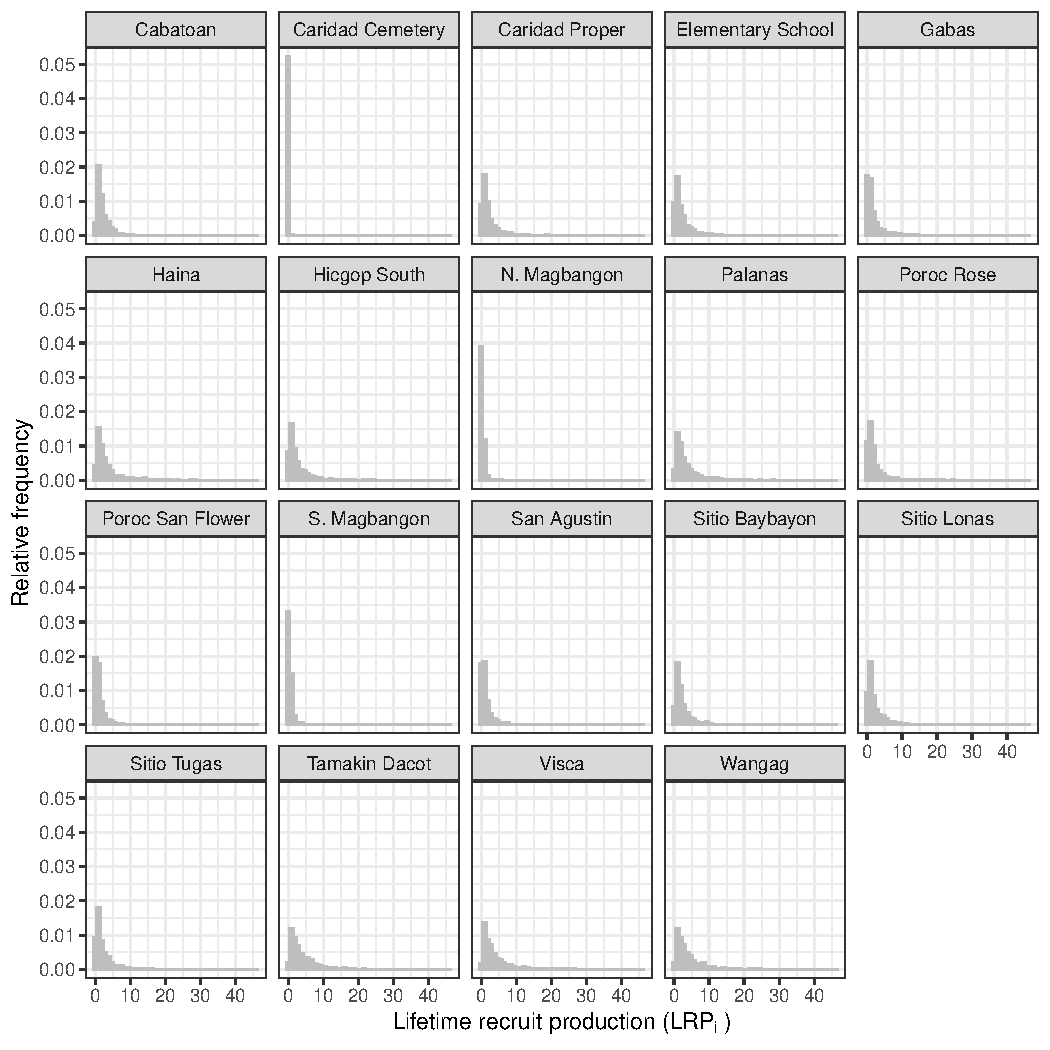
\includegraphics[width = 1.0\textwidth]{\detokenize{../Plots/FigureDrafts/LRP_by_site.pdf}}
	\caption{Site-specific lifetime recruit production ($\text{LRP}_i$) estimates. \label{APP_FIG_LRPbySite}}
\end{figure}

\begin{figure}[!htbp] % LRP and local replacement without DD compensation
	\centering
	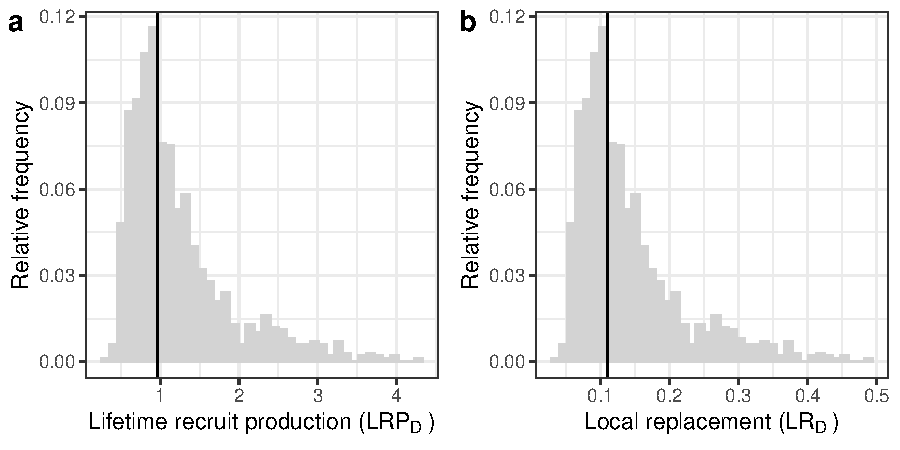
\includegraphics[width = 1.0\textwidth]{\detokenize{../Plots/FigureDrafts/APP_FIG_LRP_LocalReplacement_withoutDDconsidered_freq.pdf}}
	\caption{Estimates of a) LRP, and b) local replacement without compensating for density dependence in early life stages in our data, showing the best estimate (black solid line) and range of estimates considering uncertainty (grey) in the inputs. These estimates compare to those in \ref{FIG_Abun_LEP_LRP_LocalReplacement}c,d, where we corrected for additional mortality in early life due to density dependence. \label{APP_FIG_LRP_LocalReplacement_noDD}}
\end{figure} 

\begin{figure}[!htbp] % SP, realized connectivity matrix, NP without DD compensation
	\centering
	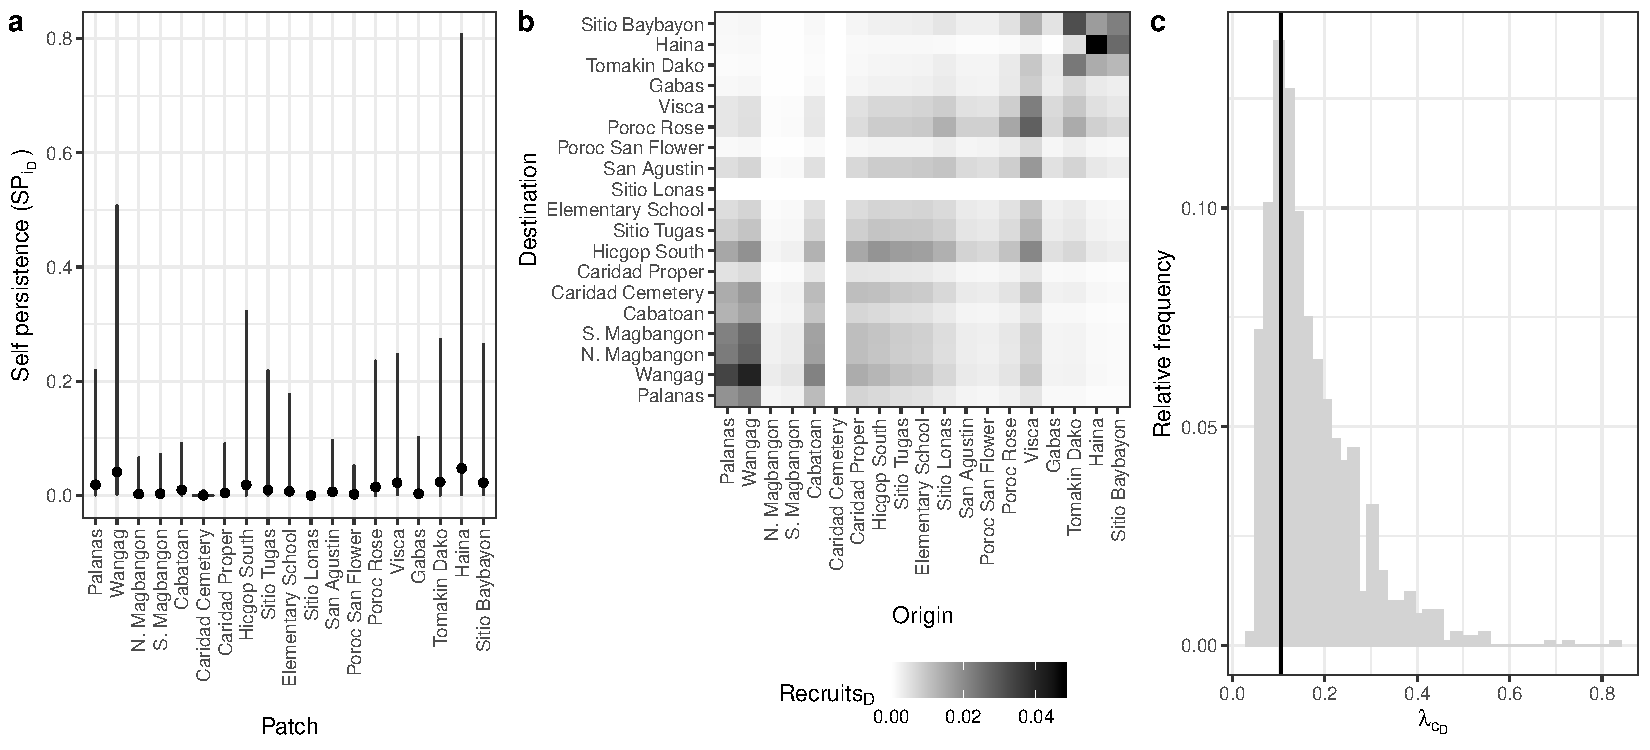
\includegraphics[width = 1.0\textwidth]{\detokenize{../Plots/FigureDrafts/APP_FIG_SP_NP_connMatrixR_withoutDDcompensation_freq.pdf}}
	\caption{Values of a) self-persistence, b) realized connectivity among patches, and c) network persistence without compensation for density-dependence in early life stages in our data. For self-persistence (a) and network persistence (c), the best estimate is shown with in black (point for (a), line for (c)) and the range of estimates considering uncertainty is shown in grey. These estimates compare to those in \ref{FIG_SP_NP_realizedCmat} where we compesated for density dependence in early life stages. \label{APP_FIG_SP_NP_realizedCmat_noDD}}
\end{figure} 

\newpage{}

Here we show the contribution of uncertainty of each input to the overall uncertainty in the values of LEP (Fig.\ \ref{APP_FIG_Uncertainty_LEP}), LRP (Fig.\ \ref{APP_FIG_Uncertainty_LEP_R}), egg-recruit survival $S_e$ (Fig.\ \ref{APP_FIG_Uncertainty_RperE}), and network persistence $\lambda_c$ (Fig.\ \ref{APP_FIG_Uncertainty_NP}). We calculated the metrics using best estimates for all inputs except the one shown and show the results as violin plots, which show vertical probability densities of the metrics across a range of values.

\begin{figure}[!htbp] % Uncertainty in LEP
	\centering
	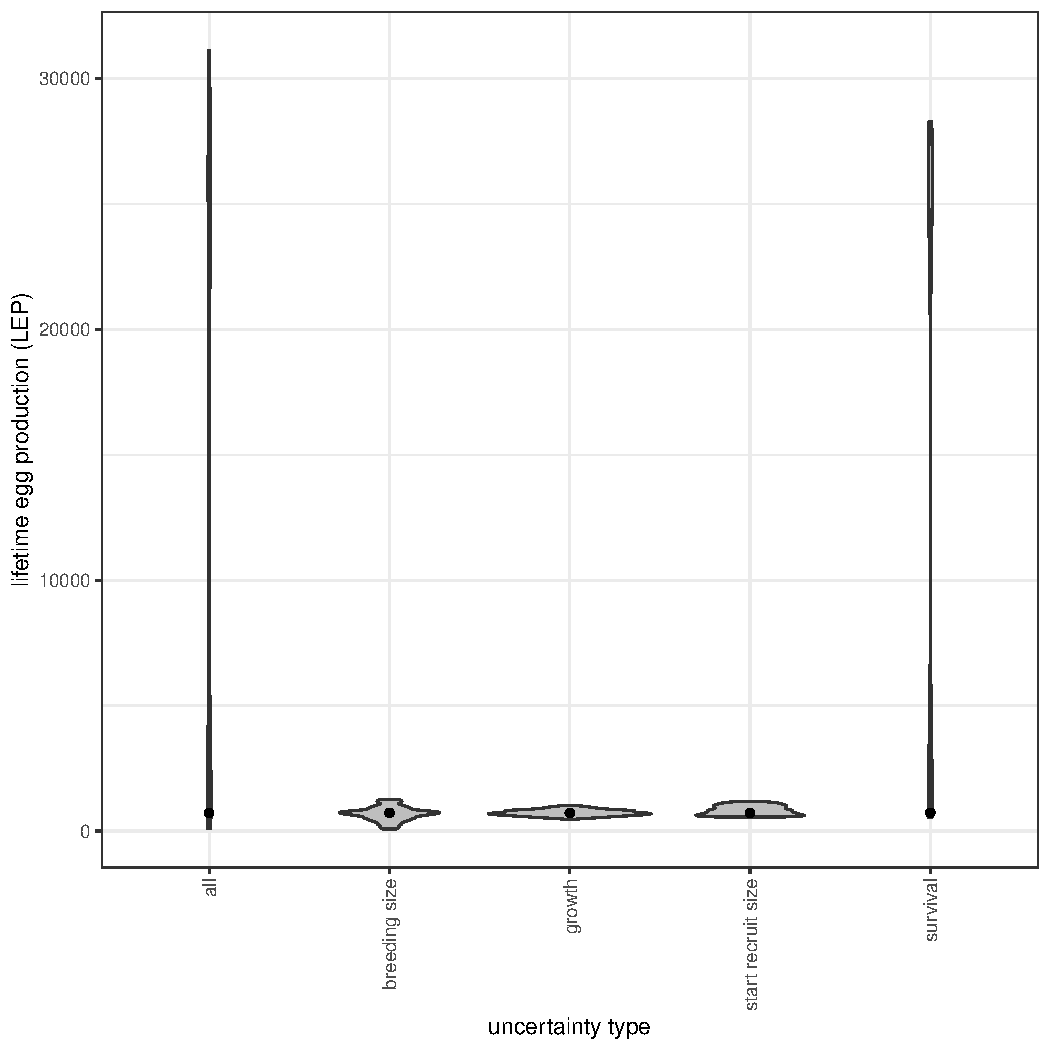
\includegraphics[width = 1.0\textwidth]{\detokenize{../Plots/FigureDrafts/LEP_uncertainty_by_param.pdf}}
	\caption{The contribution of different sources of uncertainty in LEP. \label{APP_FIG_Uncertainty_LEP}}
\end{figure}

\begin{figure}[!htbp] % Uncertainty in LEP_R 
	\centering
	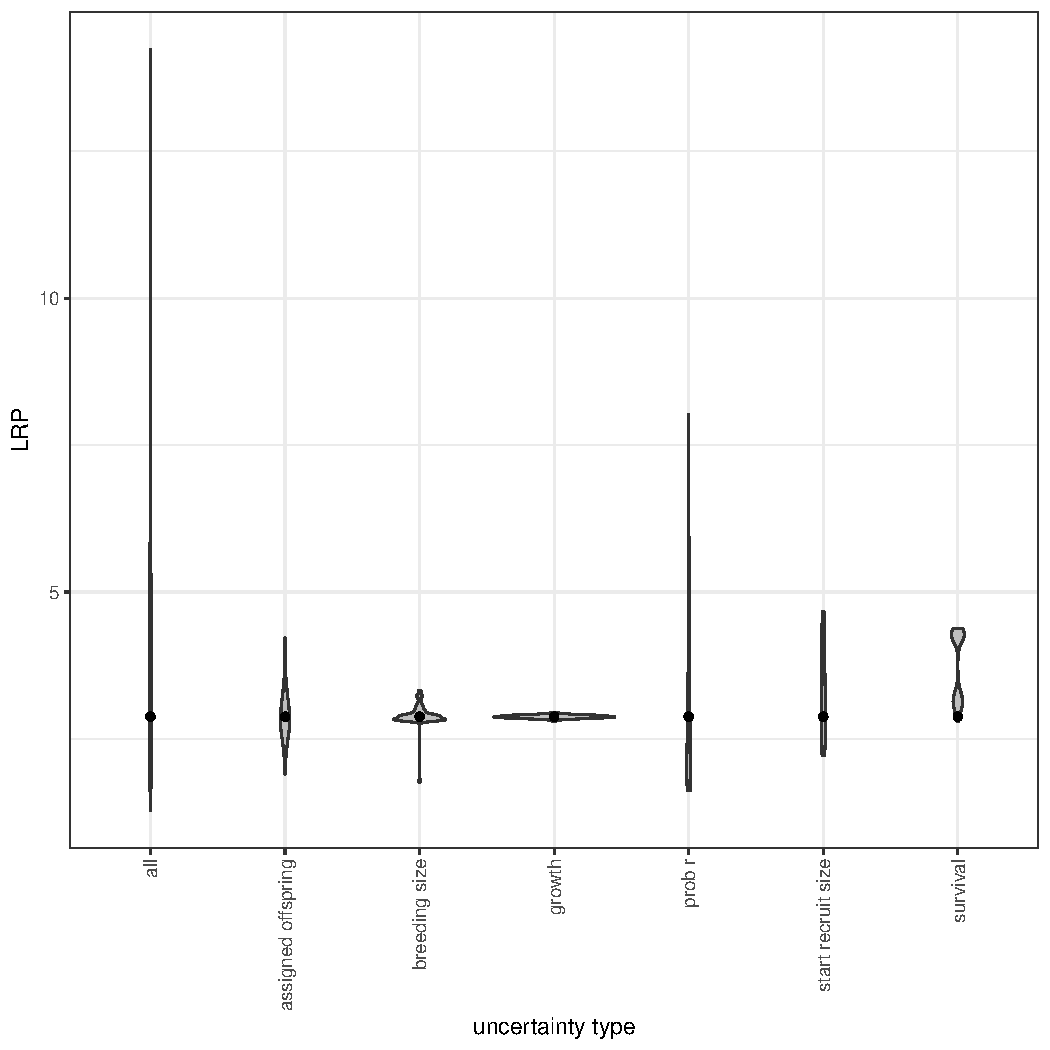
\includegraphics[width = 1.0\textwidth]{\detokenize{../Plots/FigureDrafts/LRP_uncertainty_by_param.pdf}}
	\caption{The contribution of different sources of uncertainty in LRP. \label{APP_FIG_Uncertainty_LEP_R}}
\end{figure}

\begin{figure}[!htbp] % Uncertainty in recruits-per-egg
	\centering
	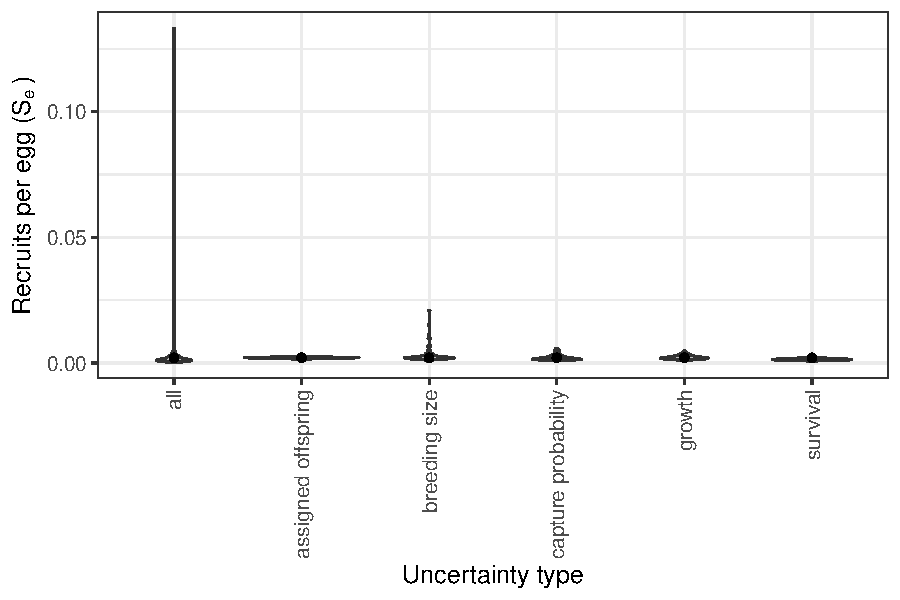
\includegraphics[width = 1.0\textwidth]{\detokenize{../Plots/FigureDrafts/RperE_uncertainty_by_param.pdf}}
	\caption{The contribution of different sources of uncertainty in egg-recruit survival. \label{APP_FIG_Uncertainty_RperE}}
\end{figure}

\begin{figure}[!htbp] % Uncertainty in NP
	\centering
	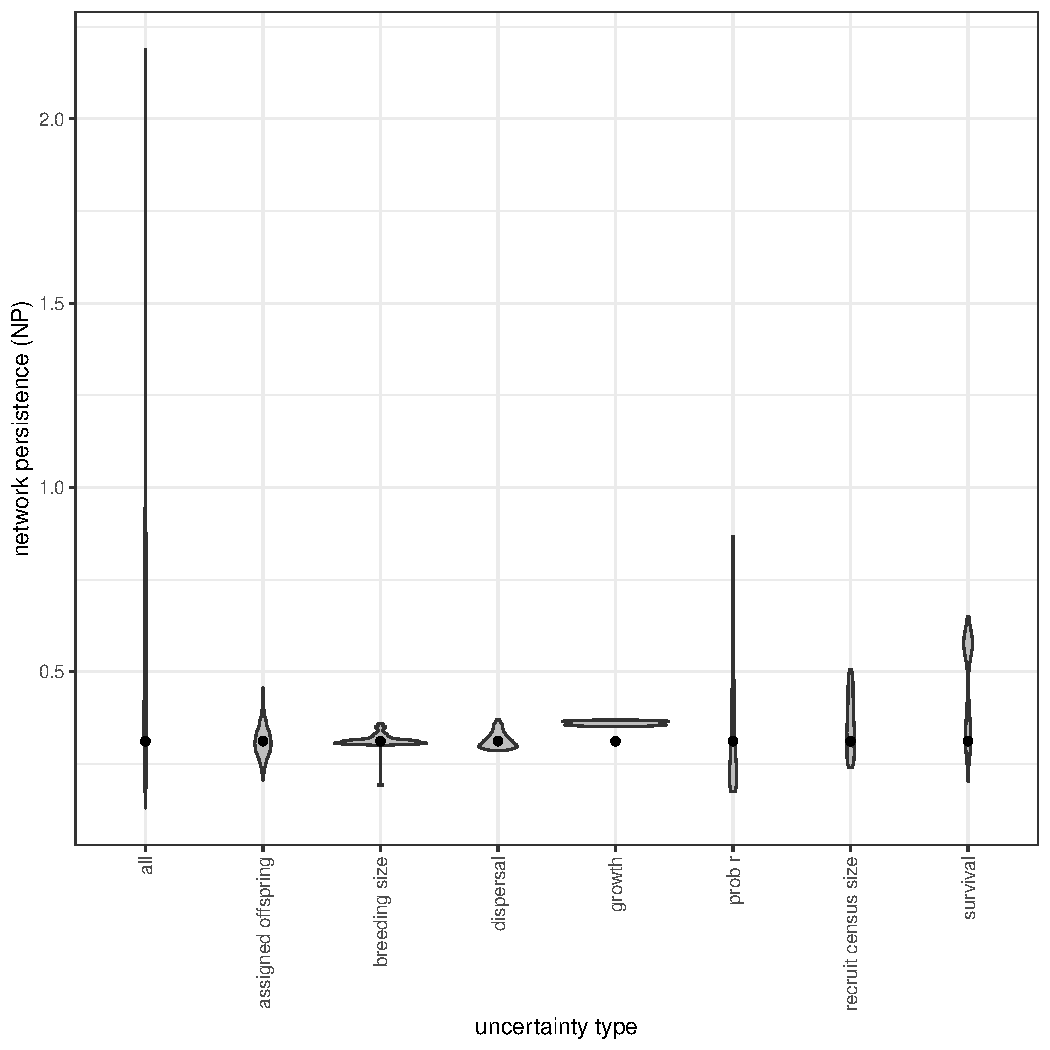
\includegraphics[width = 1.0\textwidth]{\detokenize{../Plots/FigureDrafts/NP_uncertainty_by_param.pdf}}
	\caption{The contribution of different sources of uncertainty in NP. \label{APP_FIG_Uncertainty_NP}}
\end{figure}

% \section*{Comparison to other studies}
% \subsection{Persistence metrics}

%% MOVE TO SUPPLEMENT! Malin comment: to supplement, perhaps in a section comparing to other studies, Will thinks okay to delete entirely but also okay in SI
% Our equation for SP is a modification of that used in \cite{burgess2014beyond}, which uses LEP to represent offspring produced and uses local retention (the number of surviving recruits that disperse back to the natal patch divided by the number of eggs produced by the natal patch) to capture egg-recruit survival and dispersal combined: $\text{LEP} \times \text{local retention} \geq 1$. We modify this to include egg-recruit survival in the offspring term instead, using LRP in place of LEP. %, to assess whether a particular patch $i$ is self-persistent.


%%%%%%%%%%%%%%%%%%%%%%%%%%%%%%%%%% Original supplement below, need to re-arrange into the above!

%\textit{Add details about how sometimes it is >1 if the site doesn't have metal tags? Mention plastic tags?}


% \begin{equation}
% %p(d) = e^k e^{-(e^k d)^\theta}. \label{EQN_DispKernel}
% p(d) = ze^{-(zd)^\theta}. \label{EQN_DispKernel}
% \end{equation}



% \begin{table}
% \begin{centering}
% \caption{Table showing MARK models considered and their relative AICc scores.}\label{APP_TAB_MARKmodels}
% \begin{tabular}{|p{2in}|p{2.5in}|p{0.75in}|p{0.75in}|}
% \hline 
% \textbf{Model} & \textbf{Model description} & \textbf{AICc} & \textbf{dAICc} \\ \hline
% $\phi \sim S$, $p \sim S+D$ & survival size, recapture size+distance & 3348.861 & 0 \\ \hline
% $\phi \sim S$, $p \sim D$ & survival size, recapture distance & 3359.998 & -11.1371 \\ \hline
% $\phi$, $p \sim D$ & survival constant, recapture distance & 3383.175 & 34.3141 \\ \hline
% $\phi$, $p \sim S+D$ & survival constant, recapture size+distance & 3384.959 & 36.0981 \\ \hline
% $\phi \sim t$, $p$ & survival time, recapture constant & 3408.342 & 59.4816 \\ \hline
% $\phi \sim i$, $p$ & survival site, recapture constant & 3440.842 & 91.98112 \\ \hline
% $\phi \sim i$, $p \sim S+D$ & survival site, recapture size+distance & 3440.842 & 91.98112 \\ \hline
% $\phi$, $p \sim t$ & survival constant, recapture time & 3453.609 & 104.74839 \\ \hline
% $\phi \sim S$, $p \sim S$ & survival size, recapture size & 3527.710 & 178.84940 \\ \hline
% $\phi$, $p$ & survival constant, recapture constant & 3570.908 & 222.04690 \\ \hline
% \end{tabular}
% \end{centering}
% \end{table}


% \paragraph{Recapture model} 
% The best model for log-odds recapture probability, accompanying the survival model in eqn.\ \ref{EQN_Survival}, has a size effect ($b_1 = -1.816 \pm 0.080$ SE, Fig.\ \ref{APP_FIG_RecapSizeDistEffect}a) and a negative effect of diver distance from the anemone ($b_2 = -0.171 \pm 0.021$ SE, Fig.\ \ref{APP_FIG_RecapSizeDistEffect}b), with intercept $b_{p_r} = 17.93 \pm 0.858$ SE:

% \begin{equation}
% \log(\frac{p_r}{1-p_r}) = b_{p_r} + b_1\text{size} + b_2d. \label{APP_EQN_MARK_Recapture}
% \end{equation}
% \begin{eqnarray}
% \log(\frac{\phi}{1-\phi}) &=& b_\phi + b_a\text{size} \\
% \log(\frac{p_r}{1-p_r}) &=& b_{p_r} + b_1\text{size} + b_2d. \label{EQN_Survival}
% \end{eqnarray}
%These results suggest that larger fish have higher annual survival, which is similar to survival estimates in other clownfish species (check Buston paper). 

% The negative effect of both size and distance suggest that divers are less likely to recapture larger fish and those at anemones far from areas sampled. %, with the chance of recapturing an average-sized fish falling below 5\% if a diver stays farther than XX from its home anemone.

% Add plot of distances to anems in different years?
% Add plot of effect of size and distance on recapture probability?

% From the mark-recapture analysis of tagged and genotyped fish, we estimate mean values of $L_\infty = 10.71 \text{cm}$ (range of estimates 10.50 - 10.90 cm) and $K = 0.864$ (range of estimates 0.785 - 0.944) for the von Bertalanffy growth curve parameters (eqn.\ \ref{EQN_VBL}, Fig.\ \ref{FIG_ParameterInputs}b, Table \ref{APP_TAB_Params}). For juvenile and adult (post-recruitment) survival on a log-odds scale, the best-fit model has an effect of size, with coefficient $b_a = 0.169 \pm 0.028$ SE and intercept $b_\phi = -1.83 \pm 0.231$ SE (eqn.\ \ref{EQN_Survival}). The accompanying best-fit model for log-odds recapture probability has a negative size effect and a negative effect of diver distance from the anemone (eqn.\ \ref{APP_EQN_MARKRecapture}, Fig.\ \ref{APP_FIG_RecapSizeDistEffect}).


% Range of parameters used as input for uncertainty runs

% \begin{figure}[H] % Range of parameter inputs for uncertainty runs
% 	\centering
% 	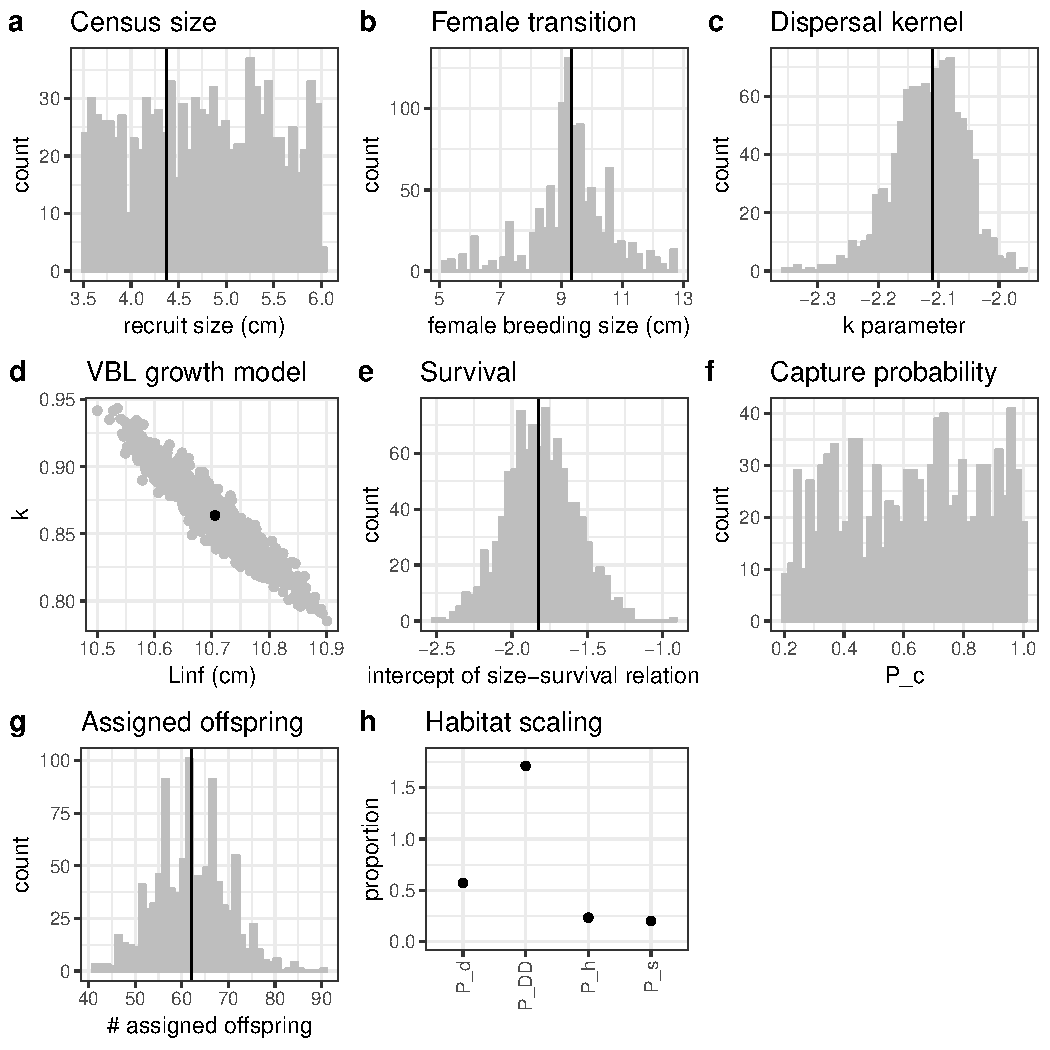
\includegraphics[width = 1.0\textwidth]{\detokenize{../Plots/FigureDrafts/Uncertainty_inputs.pdf}}
% 	\caption{Range of parameter inputs for uncertainty runs with all uncertainty included: a) $\text{size}_\text{recruit}$, the census size at which fish are considered to have recruited after egg-recruit survival occurs; b) $L_f$, the size at which fish transition from male to female and their reproductive output is included in the estimate of lifetime egg production (LEP); c) $k_d$, the scale parameter in the dispersal kernel; d) the parameters $L\infty$ and $K$ of the von Bertalanffy growth model; e) the intercept $b_\phi$ of the adult size-dependent survival relationship; f) $P_c$, the probability of capturing a fish; g) number of offspring assigned back to parents in the parentage analysis; h) factors that scale the number of estimated recruits from our site based on density-dependence in settler success (DD), proportion of the dispersal kernel captured by our sampling region ($P_d$), the cumulative proportion of our sites we sampled over time ($P_h$), and the proportion of our sampling area that is habitat ($P_s$). \label{APP_FIG_UncertaintyInputs}}
% \end{figure}

% % Relationships among parameters - MAKE A NEW ONE OF THESE???

% \begin{figure}[H] % 4 relationships among parameters
% 	\centering
% 	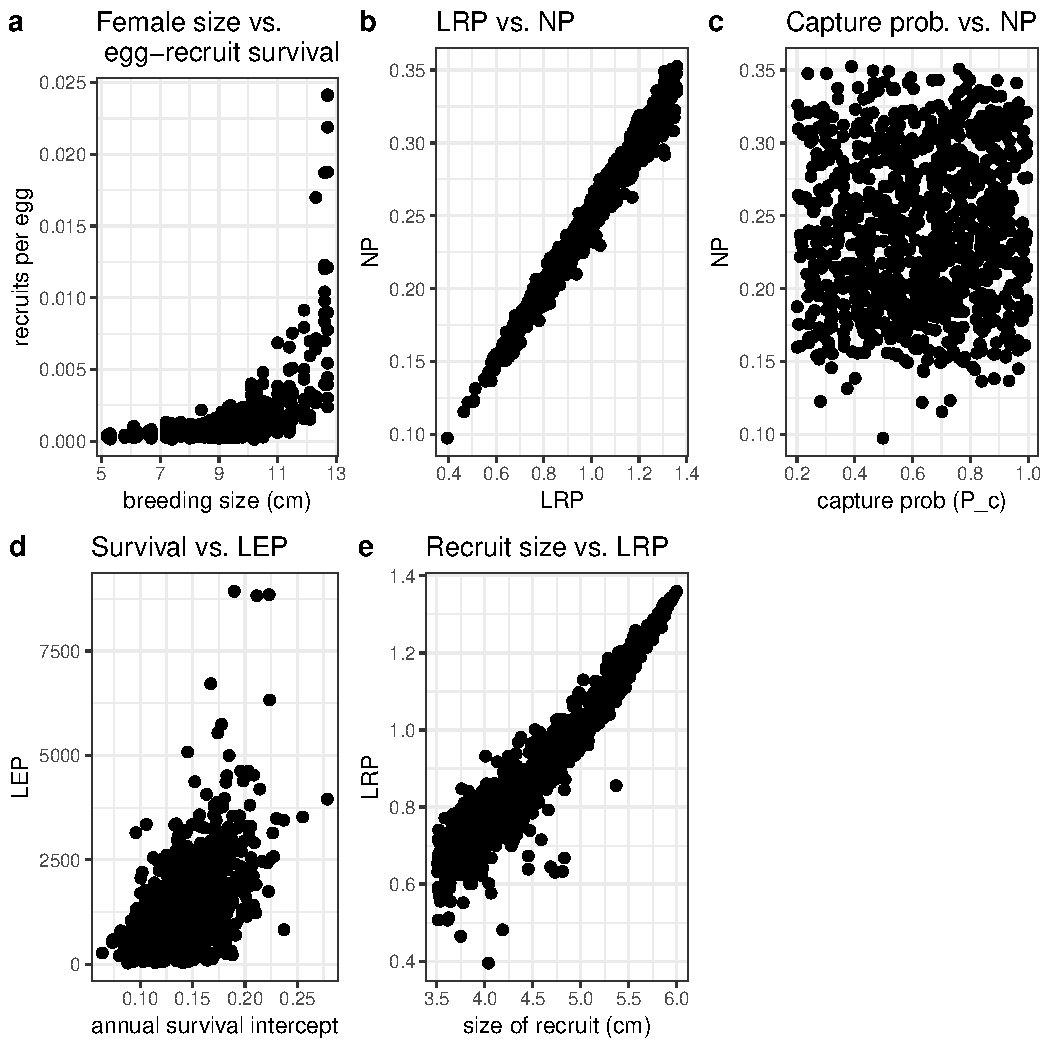
\includegraphics[width = 1.0\textwidth]{\detokenize{../Plots/FigureDrafts/Param_metric_relationships.pdf}}
% 	\caption{Relationships among parameters and metrics. a) We only count reproductive effort by fish in the female stage so the higher the transition size to breeding female, the fewer eggs parents are considered to produce, which increases the estiamted egg-recruit survival. b) LRP strongly affects NP by changing the number of potential recruits dispered through the connectivity matrix. c) The probability of capturing a fish does not have a clear relationship to NP. d) LEP is higher with higher survival estimates because fish are more likely to survive longer as reproducing adults. e) The size we consider to be a recruit marks the transition of mortality included in egg-recruit survival to mortality being captured by annual adult survival. Because we do not have the data to change egg-recruit survival to account for different recruit sizes, increasing the recruit size increases LRP by wrapping more mortality into the egg-recruit survival estimate, rather than LEP. \label{APP_FIG_ParamMetricRelationships}}
% \end{figure} % Think about a better way to explain (e) and whether we should even include it.

% \subsection{Effects of different types of uncertainty on metrics}

% Here we show the contribution of uncertainty in each input to the overall uncertainty in the values of LEP (Fig.\ \ref{APP_FIG_Uncertainty_LEP}), $\text{LRP}_{DD}$ (Fig.\ \ref{APP_FIG_Uncertainty_LEP_R}), egg-recruit survival $S_{e_{DD}}$ (Fig.\ \ref{APP_FIG_Uncertainty_RperE}), and network persistence $\lambda_{c_{DD}}$ (Fig.\ \ref{APP_FIG_Uncertainty_NP}). We calculate the metrics using best estimates for all inputs except the one shown and show the results as violin plots, which show vertical probability densities of the metrics across a range of values.


\newpage{}

%\bibliography{../../../BibTexReferences}
\bibliography{BibTexReferences}
\bibliographystyle{plainnat}

% NEED TO ADD IAN IMAGES REFERENCES
% SCUBA diver in scaling up recruits figure: \url{https://ian.umces.edu/imagelibrary/displayimage-5410.html}, downloaded 11/22/19
\end{document}